 % Default language option is [thaithesis]. The other possible option is [engthesis].
% Default format option is [ugrad]. Other possible options are [master,doctor].
\documentclass[a4paper,thaithesis]{ubu}

% List all required packages here
% ทุก package รวมไว้ที่เดียว 
\usepackage{coding}

%%------------------------------------------------------------
%%-               SETTING THESIS PARAMETERS                  -
%%------------------------------------------------------------

%%-----------------   ชื่อโครงงาน                 -----------%%
%% หัวข้อโครงงาน {ไทย} {English}
\thesistitle                 
{ระบบสแกนใบหน้าสำหรับเเคชเชียร์} 
{Recognition for cashier} 

%%-----------------   ผู้พัฒนาโครงงาน              -----------%%
%% คำนำหน้า {ไทย} {English}
\authortitle                            
{นางสาว}                           
{Miss}                             
%% ชื่อสกุล {ไทย} {English}
\thesisauthor                           
{ภัทราภรณ์ อินทา}                         
{Pattaraporn Inta}            

              

%%----------------   อาจารย์ที่ปรึกษาโครงงาน        ----------%%
\advisor   
{อาจารย์ ดร.ไพชยนต์ คงไชย}       
{ดร.ไพชยนต์ คงไชย}                 
{Phaichayon Kongchai , Ph.D.}    
{PAICHAYON KONGCHAI , Ph.D.}      

%%----------------   อาจารย์ที่ปรึกษาโครงงาน (ถ้ามี)  ----------%%
%\coadvisor
%{อาจารย์ ดร.ชื่อร่วม สกุล}               
%{ดร. ชื่อร่วม สกุล}                          
%{Cofirstname Lastname, Ph.D.}  
%{COFIRTNAME LASTNAME, Ph.D.}          

%%----------------   ข้อมูลสถาบัน                  ----------%%
%% คณะ {ไทย} {English}
\faculty
{วิทยาศาสตร์}                          
{Science}                           
%% ภาควิชา {ไทย} {English}
\department                             
{คณิตศาสตร์ สถิติ และคอมพิวเตอร์}                      
{Mathematics Statistics and Computer}                  

%%----------------   ข้อมูลหลักสูตรและรายวิชา        ----------%%
%% ชื่อหลักสูตร
\fieldofstudy                           
{วิทยาการคอมพิวเตอร์}                      
{Computer Science}                  
%% ชื่อปริญญา
\degree                                 
{วิทยาศาสตรบัณฑิต}                   
{Bachelor of Science}                  
%% ปีการศึกษาที่ทำโครงงาน
\academicyear{2562}                     
%% รหัสประจำตัวนักศึกษา
\authorid{59110440309}                   
%% รหัสวิชา
\subjID{1104494}							
%% ชื่อวิชา
\subjName								
{โครงงานวิทยาศาสตร์}
{Senior Project}

%%----------------   หัวหน้าภาควิชา            ----------%%
\deanname                               
{ผศ.ดร. สุพจน์ สีบุตร}                       
{ Asst. Prof. Supot Seebut, Ph.D.}     

%%----------------   รายชื่อคณะกรรมการสอบโครงงาน -------%%
\committee                              
{
\CommitteeBlockAdvisor                  
\CommitteeBlockCoAdvisor                
\CommitteeBlock{กรรมการ}{ดร. วราวุฒิ ผ้าเจริญ} 
\CommitteeBlock{กรรมการ}{ดร. ทศพร จูฉิม} } 
}

%%-------------------------------------------------------------------------------
%%-                               DOCUMENT                                      -
%%-------------------------------------------------------------------------------
\begin{document}
% หน้าปกภาษาไทย - Thai Cover
\makethaicover
\newpage

% หน้าปกภาษาอังกฤษ - English Cover
%\makeenglishcover
%\newpage

% หน้ารายชื่อคณะกรรมการสอบ - Committee page
%\makecommittee
\ThaiCommittee
\newpage

% หน้ากิตติกรรมประกาศจากไฟล์ acknowledgement.tex
\begin{acknowledgements}
	การพัฒนาโครงงานระบบ สแกนใบหน้าสำหรับเเคชเชียร์ สำเร็จลุล่วงได้ด้วยความกรุณาแลความช่วยเหลือจากหลายๆ ท่าน ข้าพเจ้าขอขอพระคุณทุกท่าน ที่มีส่วนร่วมในการพัฒนาโครงงานนี้
	
    ขอขอบพระคุณอาจารย์ที่ปรึกษา  ดร.ไพชยนต์ คงไชย  อาจารย์ที่ปรึกษาโครงงานที่ได้แนะนำทฤษฎีและแนวทางในแก้ปัญหาต่าง ๆ  ที่เกิดขึ้นระหว่างการพัฒนาระบบ อีกครั้งยังคอยตรวจสอบความก้าวหน้าของการทำงานเป็นระยะ ๆ รวมทั้งสร้างกำลังใจให้ผู้พัฒนาอยู่เสมอ

  
    
   ขอขอบพระคุณเจ้าหน้าที่ภาควิชาคณิตศาสตร์ สถิติและคอมพิวเตอร์ ที่คอยเอื้อยอำนวยความสะดวกทั้งเรื่องอุปกรณ์และสถานที่ต่อการปฏิบัตงานของผู้พัฒนา
   
 
  ขอกราบขอบพระคุณบิดา มารดา ที่คอยให้กำลังใจ คอยให้ความรักและความห่วงใยเสมอมา
  ตลอดจนคอยช่วยเหลือทุนทรัพย์ทางด้านการศึกษาและอุปกรณ์ในการพัฒนาโครงงาน
    
\end{acknowledgements}

\begin{flushright}
    นางสาวภัทราภรณ์  อินทา
    \\
    เมษายน 62
\end{flushright}

\newpage

% หน้าบทคัดย่อภาษาไทยจากไฟล์ abstractthai.tex
\begin{thaiabstract}
	แอปพลิเคชั่นสแกนใบหน้าสำหรับเเคชเชียร์(Face Recognition for  Cashier) แอปพลิเคชั่นสำหรับการชำระเงินของลูกค้า โดยจะมีการสแกนใบหน้าเพื่อเก็บข้อมลูของลูกค้าที่มาใช้บริการและชำระสินค้าในครั้งแรกเเล้วต้องการสมัครสมาชิก และการสแกนใบหน้านี้จะใช้เเทนบัตรสมาชิกสำหรับลูกค้าที่เป็นสมาชิกแล้ว เมื่อสแกนใบหน้าเเล้วจะมีการแสดงข้อมูลในระบบ จะประกอบด้วย ประวัติลูกค้า เเต้มสะสม(point) สำหรับลูกค้าที่เป็นสมาชิกเท่านั้น และยังมีการแสดงประวัติรายการสั่งซื้อ สว่นที่ไม่เป็นสมาชิกจะไม่มีการเก็บข้อมูลลูกค้า จะสามารถสั่งสินค้าเพียงเท่านั้น จุดเด่นของแอปพลิเคชั่นจะมีเนื้อหาชี้ให้เห็นได้ชัดเจนถึงการสแกนใบหน้าเพื่อเก็บข้อมูลของลูกค้าเเละบันทึกข้อมูล ประวัติการสั่งซื้อนี้สินค้าของลูกค้าทุกครั้ง เพื่อนำไปใช้ในฟังก์ชั่นแนะนำเมนูให้ลูกค้าเพื่อช่วยให้ลูกค้าตัดสินใจได้ง่ายขึ้น

\noindent
\\คำสำคัญ: เว็บแอปพลิเคชัน 
\end{thaiabstract}

\newpage

% หน้าบทคัดย่อภาษาอังกฤษจากไฟล์ abstractenglish.tex
\begin{englishabstract}
Face Recognition for Cashier, an application for payment of customers There will be a face scan to collect the information of customers who use the service and pay the product for the first time. And this face scan will be used as a membership card for members already Once the face has been scanned, data will be displayed in the system, consisting of customer history Accumulate (point) for customers that are members only And also showing order history for the past 1 month. Non-members will have order history only And the customer's face only There will be no accumulation (point) when passing the face scan. And the system will display the customer information The order history will show a list of past products. And to the order function And the menu navigation function for customers In order to help customers make decisions quickly Customers must go through a face scan before accessing the various functions. The highlight of the application is the content that clearly shows the face scan to collect customer data and save data. This purchase history of every customer's product. To be used in the menu suggestion function for customers to help customers make easier decisions


\noindent
Keywords: Web Application
\end{englishabstract}


\newpage


% คำสั่งสร้างรายการสารบัญ
\tableofcontents
\newpage
% คำสั่งสร้างรายการตาราง
\listoftables
\newpage
% คำสั่งสร้างรายการภาพอ้างอิง
\listoffigures
\newpage

% คำสั่งรวมไฟล์ต่างๆในโครงการ แยกรายบท
\chapter{บทนำ}

\section{ที่มาและเหตุผล }
   ปัจจุบันเทคโนโลยีเกี่ยวกับการประมวลผลภาพได้ถูกนำไปประยุกต์ใช้มากมาย เช่น การสแกนใบหน้าเพื่อเข้าใช้งานโทรศัพท์มือถือ การสเเกนลายนิ้วมือ อีกทั้งการนำไปจดจำใบหน้าเพื่อเก็บข้อมูล เเละนำข้อมูลมาใช้ในครั้งต่อไป  และเทคโนโลยีการประมวลผลภาพนี้ยังเป็นที่นิยมในสังคมตอนนี้ เพราะมันง่ายต่อการใช้งาน ไม่ต้องมีอุปกรณ์ที่ช่วยในการเข้าถึงข้อมูล ใช้เเค่ใบหน้าในการตรวจสอบ  อีกทั้งยังมีการนำ Machine learning มาใช้ในการช่วยตัดสินใจในการสั่งสินค้าของลูกค้า  



ด้วยเหตุนี้จึงมีความประสงค์ที่จะนำเทคโนโลยีการประมวลผลภาพมาใช้ เพื่อที่จะบันทึกใบหน้าของลูกค้าที่มาชำระเงิน เพื่อนำข้อมูลมาใช้ในครั้งต่อๆไป แทนการใช้อุปกรณ์ที่ช่วยในการเข้าถึงข้อมูลลูกค้าที่ยุ่งยาก เเละสะดวกต่อลูกค้าเพื่อช่วยแก้ไขการลืมบัตรสมาชิก สะกดชื่อไม่ถูก ลืมเบอร์โทรศัพท์ที่ใช้ในการสมัคร  และช่วยในการตัดสินใจสั่งสินค้าได้รวดเร็วขึ้น โดยใช้ Decision Tree มาช่วยในการเเนะนำเมนู 


\section{วัตถุประสงค์}
\begin{enumerate}
	\item เพื่อออกแบบเเละพัฒนาแอปพลิเคชั่น จดจำใบหน้าในการชำระเงิน 
	\item  เพื่อดูข้อมูล และประวัติการสั่งซื้อที่ผ่านมาของลูกค้าได้ โดยผ่านการสแกนใบหน้าลูกค้า    
	\item เพื่อแนะนำ เมนูแก่ลูกค้า เวลาที่ลูกค้าไม่รู้ว่าจะสั่งอะไร 
	\item ใช้การสแกนใบหน้าแทนการใช้บัตรสมาชิก 
    \item ช่วยในการตัดสินใจ การสั่งซื้อสินค้าของลูกค้าได้     
    \item เพื่อช่วยลดทรัพยากรที่ใช้ในการผลิตบัตรสมาชิก และอปุกรณ์อื่นๆที่ต้องใช้ร่วมกัน
\end{enumerate}
\section{ขอบเขตของโครงงาน}
\begin{enumerate}
	\item ใช้สำหรับพนักงานเเคชเชียร์เท่านั้น
	\item เพื่อดูข้อมูล และประวัติการสั่งซื้อที่ผ่านมาของลูกค้าได้อย่างรวดเร็ว โดยผ่านการสแกนใบหน้าลูกค้าเท่านั้น
	\item ไม่ต้องมีบัตร ก็สามารถดูข้อมูลต่างๆของลูกค้าได้ จากการสแกนใบหน้า
    \item 	ช่วยในการตัดสินใจการสั่งซื้อสินค้าของลูกค้าได้ 
    \item พนักงานเเคชเชียร์สามารถสั่งสินค้าให้ลูกค้าได้เท่านั้น
		 \begin{itemize}
		 	
		 	
	
	\end{itemize}
\end{enumerate}
\section{ประโยชน์ที่คาดว่าจะได้รับ}
\begin{enumerate}
	\item ช่วยลดปริมาณทรัพยากรที่ใช้ในการผลิตบัตร 
	\item ช่วยให้พนักงานเเคชเชียร์ทำงานได้ถูกต้องและเเม่นยำ 
   \item ช่วยลดปัญหาลูกค้าลืมบัตรสมาชิก ลืมชื่อที่ใช้สมัครสมาชิก
   \item สามารถแนะนำเมนูให้ลูกค้าโดยเทียบจากประวัติการสั่งซื้อ 
\end{enumerate}
\section{เครื่องมือที่ใช้ในการพัฒนา (Development tools)}
\subsection{ฮาร์ดเเวร์}
\begin{enumerate}
	\item สมาร์ทโฟน (Smart phone)
		\begin{itemize}
			\item ทำงานบนระบบปฏิบัติการแอนดรอย์เวอร์ชัน 5.0 หรือ API Level 21
			\item หน่วยประมาลผลกลาง Mediatek MT6753 Octa-core ความเร็ว 1.3 กิกะเฮิร์ตซ์ (Gigahertz, GHz)
			\item หน่วยประมวลผลกราฟฟิกอย่างน้อย Mali-T720MP3
			\item หน่วยความจำหลักอย่างน้อย 2 กิกะไบต์ (Gigabyte, GB)
			\item หน่วยความจำสำรองอย่างน้อย 16 กิกะไบต์ (Gigabyte, GB)
			\item หน้าจอแสดงผลความละเอียดอย่างน้อย 1080 x 1920 พิกเซล  (Pixel)
			\item หน้าจอแสดงผลขนาดอย่างน้อย 5 นิ้ว
			\item กล้องถ่ายรูปความละเอียดอย่างน้อย 13 เมกกะพิกเซล (Magapixel)
		\end{itemize}
	
	\item เครื่องคอมพิวเตอร์ส่วนบุคคล (Personal computer)
		\begin{itemize}
			\item  ทำงานบนระบบปฏิบัติการ Elementary os พื้นฐานการทำงานบน Linux
			\item  หน่วยประมวลผลกลาง Intel Core i3-3217U ความเร็ว 1.80 กิกะเฮิร์ตซ์ (Gigahertz, GHz)
			\item  หน่วยประมวลผลกราฟฟิก NVIDIA GeForce GT 720M ความจำ 2 กิกะไบต์ (Gigabyte, GB) 
			\item  หน่วยความจำหลัก 4 กิกะไบต์ (Gigabyte, GB)
			\item  หน่วยความจำสำรอง 120 กิกะไบต์ (Gigabyte, GB)
		\end{itemize}
\end{enumerate}

\subsection{ซอฟต์แวร์ (Software)}
\begin{enumerate}
	\item Visaul Studio Code เป็นโปรแกรมสำหรับพัฒนาเว็บเเอปพลเคชั่น พัฒนาด้วยภาษา HTML, JavaScript, Python เเละ Java 
	\item Django เป็น Framework ที่ใช้สำหรับสร้าง UI สำหรับระบบ หรือเรียกอีกอย่างว่า Backend Framework ใช้สำหรับเป็นเว็บเซิฟเวอร์ (Web Server)  
	\item OpenCv เป็นไลบรารีฟังก์ชันการเขียนโปรแกรมที่มุ่งเน้นไปทาง การเเสดงผลแบบเรียลไทม์
	ซึ่งนำมาใช้ในส่วนของการสแกนใบหน้า
	\item Machine Learning ในส่วนของการเรียนรู้ของอัลกอริทึม Association Rule	
	\item Sqlite3 เป็นตัวจัดการฐานข้อมูล

\end{enumerate}

\newpage
\subsection{แผนการดำเนินการ}
	ในการสร้างระบบสแกนใบหน้าสำหรับเเคชเชียร์ ผู้พัฒนาได้แบ่งขั้นตอนการดำเนินงานไว้ด้วยกัน 7 ขั้นตอน ดังต่อไปนี้

%\begin{landscape}
%\sffamily
\begin{table}[H]
	\noindent
	\caption{ขั้นตอนการดำเนินงาน}
	\begin{ganttchart}[
		canvas/.append style={fill=none, draw=black!5, line width=.75pt},
		vgrid={*2{draw=black!7, line width=.75pt}},
		title label font=\bfseries\footnotesize,
		bar label node/.append style={
			align=left,
			text width=width("7. Functional Testing On")},
		bar/.append style={draw=none, fill=black!63}
		]{1}{22}
		\gantttitle{2562}{3}
		\gantttitle{2563}{5}\\
		\gantttitle{ต.ค.}{2}
		\gantttitle{พ.ย.}{2}
		\gantttitle{ธ.ค.}{2} 
		\gantttitle{ม.ค.}{2}
		\gantttitle{ก.พ.}{2}
		\gantttitle{มี.ค.}{2}
		\gantttitle{เม.ย.}{2}
		\gantttitle{พ.ค.}{2}
		 \\
		\ganttbar{1.ศึกษาความเป็นไปได้}{1}{4} \\
		\ganttbar{2.เสนอหัวข้อโครงงาน}{5}{6} \\
		\ganttbar{3.ศึกษาค้นคว้าข้อมูล}{7}{8} \\
		\ganttbar{4.ศึกษาการใช้เครื่องมือ}{7}{10} \\
		\ganttbar{5.วิเคราะห์และออกแบบ}{7}{12} \\
		\ganttbar{6.เขียนโปรแกรม}{7}{13} \\
		\ganttbar{7.ทดสอบและแก้ปัญหา}{13}{14} \\
		\ganttbar{8.จัดทำเอกสาร}{13}{16} \\
	\end{ganttchart}
	\label{tab:ganttchart}
\end{table}
%\end{landscape}
%TODO แก้เทมเพลตเอาชื่อตารางไว้ด้านบน
 
\chapter{ทฤษฎีที่เกี่ยวข้อง}
บทนี้จะเป็นรายละเอียดเกี่ยวกับทฤษฎีและงานวิจัยที่เกี่ยวของกับการพัฒนาโปรแกรมในครั้งนี้ โดยที่แต่ละหัวข้อจะมีความสัมพันธ์กันเป็นลำดับ โดยหัวข้อที่หนึ่งจะแนะนำความรู้เรื่อง Python เพื่อให้เข้าใจพื้นฐานเบื้องต้นเกี่ยวกับที่มาของโครงงาน หัวข้อที่สองที่สามจะช่วยเตรียมให้ผู้อ่านเข้าใจเทคโนโลยที่ใช้ในการออกแบบและพัฒนา ส่วน ...

\section{ความรู้พื้นฐานเกี่ยวกับ Python}
	Python  คือ ภาษาเขียนโปรแกรมระดับสูงที่ใช้กันอย่างกว้างขวางในการเขียนโปรแกรมสำหรับวัตถุประสงค์ทั่วไป ภาษา Python นั้นเป็นภาษาแบบ Interprete ที่ถูกออกแบบให้โค้ดอ่านได้ง่ายขึ้น และโครงสร้างของภาษานั้นจะทำให้โปรแกรมเมอร์สามารถเข้าใจแนวคิดการเขียนโค้ด โดยใช้บรรทัดที่น้อยลงกว่าภาษาอย่าง C++ และ Java ซึ่งภาษานั้นถูกกำหนดให้มีโครงสร้างที่ตั้งใจให้การเขียนโค้ดเข้าใจง่าย ทั้งในโปรแกรมเล็กไปจนถึงโปรแกรมขนาดใหญ่ คุณลักษณะเด่นของภาษา Python 
    \begin{enumerate}
    	\item สนับสนุนแนวแบบคิดออปเจกต์โอเรียนเทด หรือ OOP (Object Oriented Programming)
    	\item เป็น Open Source
    	\item โค้ดที่เขียนด้วย Python สามารถนำไปรันบนระบบปฏิบัติการได้หลากหลาย
    	\item สามารถประมาลผมทางด้านวิยาศาสตร์ และวิศวกรรมศาสตร์ได้อย่างมีประสิทธิภาพ
    	\item มีฟังก์ชันสนับสนุนฐานข้อมูล เช่น MySQL, Sybase, Oracle , Informix, ODBC และอื่นๆ
    	\item มี Library สนับสนุนด้านการสร้างภาพกราฟฟิก ตลอดจนบันถึกไฟล์ในรูปแบบต่างๆ ได้อย่างสะดวกและมีประสิทธิภาพ
    	\item มี Library สนับสนุนด้านปัญญาประดิษฐ์
    \end{enumerate}
    

	\section{ความรู้พื้นฐาน Django Framework}
	Django Framework  คือ ชุดเครื่องมือ Framework สำหรับ การพัฒนาเว็บไซต์ด้วยภาษา Python ซึ่งความเป็นจริงแล้วทุกวันนี้มี Framework สำหรับการเขียนเว็บไซต์ด้วยภาษา Python ค่อนข้างเยอะ ซึ่ง Django Framework เป็นหนึ่งใน Framework สำหรับการพัฒนาเว็บไซต์ และทำเว็บไซต์ด้วยภาษา Python ด้วยเช่นกัน โดยปัจจุบันภาษา Python นั้นค่อนข้างได้รับความนิยมเพิ่มมากขึ้น  Django Framework \cite{django} มีคุณสมบัติดังนี้
	
	\begin{enumerate}
		\item Object-relational mapper คือ การกำหนด Data Model ในภาษา Python เพื่อการทำงานด้านข้อมูล และสนับสนุน Dynamic database-access API
		\item Automatic admin interface คือ ส่วนของการสร้าง Interface อัตโนมัติสำหรับการ add, edit , delete และ search ด้วย Django Framework
		\item  Elegant URL design คือ การทำให้ URL มีความสวยงาม สั้น กระชับ และสื่อความหมายของหน้านั้น ๆ ได้อย่างชัดเจน เหมาะสมกับการทำ SEO ในปัจจุบัน
		\item Template system คือ Django นั้นมีการออกแบบ Template Language เพื่อการเขียนแยกส่วนระหว่าง Design และ Business Logic
		\item Cache system คือ ส่วนของการบันทึก หรือจัดการข้อมูลที่มีการดาวน์โหลดไปแล้ว เพื่อเพิ่มประสิทธิภาพการทำงานของเว็บไซต์ด้านความเร็ว และด้านอื่น ๆ
		\item Internationalization คือ Django สนับสนุน Application ที่มีความหลากหลายด้านภาษาในการแสดงผล
	\end{enumerate}
	รูปแบบ MVC ของ Django   เรียกอีกอย่างว่า MTV คือ Model Template View ดังรูปที่  \ref{Fig:Django}
	
	\begin{figure}[H]
		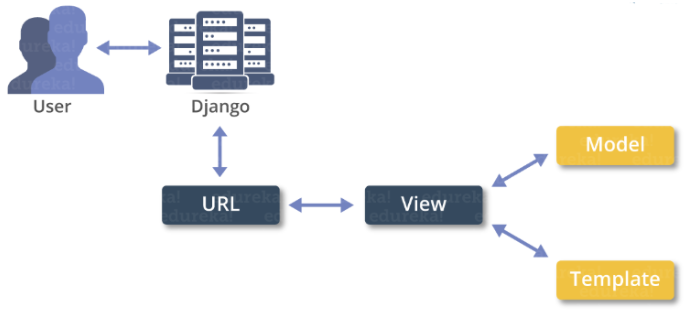
\includegraphics[width=\columnwidth]{Figures/insect2/django}
		\caption{รูปแบบ MVC ของ Django}{ที่มา: https://www.edureka.co/blog/django-tutorial/}
		\label{Fig:Django} 
	\end{figure}
	
	
	
    \end{itemize}
	
\section{ความรู้พื้นฐานเกี่ยวกับ Bootstrap}
Bootstrap  คือ Front-end Framework ที่ช่วยให้สามารถสร้างเว็บแอปพลิเคชันได้อย่างสวยงาม ตัว Bootstrap มีทั้ง CSS Component และ JavaScript Plugin ให้เรียกใช้งานได้ และยังถูกออกแบบมาให้รองรับการทำงานแบบ Responsive Web ซึ่งทำให้ การพัฒนาเว็บแค่ครั้งเดียวสามารถนำไปใช้งานบนเบราเซอร์ใน มือถือ แท็บเล็ต และคอมพิวเตอร์ ได้ และผู้พัฒนาไม่ต้องมีความรู้ด้าน CSS มาก  สามารถสร้างเว็บที่สวยงามได้เช่นกัน

\section{ความรู้พื้นฐานเกี่ยวกับ OpenCV(OpenSourceComputerVision)}
OpenCV  เป็น Library ที่รวบรวมฟังก์ชันสำหรับการประมวลผลภาพและคอมพิวเตอร์วิทัศนศาสตร์ ไว้เป็นจำนวนมากอยู่ภายใต้ใบอนุญาต BSD ซึ่งสามารถใช้ได้ฟรีทั้งทางด้าน การศึกษาและทางการค้า เนื่องจากนี้ยังมีการประยุกต์ใช้งาน OpenCV  ในแบบต่างๆ ได้แก่ ระบบตรวจจับใบหน้า (Face Detection) การจดจำใบหน้า (Face Recognition) การติดตามวัถตุ (Object Tracking) การเรียนรู้ของเครื่อง (Machine Learning) เป็นต้น

\subsection{การประมวลผลภาพ (Image Processing)}
การประมวลผลภาพคือการนำรูปที่มีอยู่แล้ว หรือรูปที่รับเข้ามาจากอุปกรณ์ต่างๆ หรือรูป ที่มีอยู่มาประมวลผลเพื่อหาลักษณะเด่นบางประการของรูปที่มีอยู่ หรืออาจจะเป็นการตีความ หมายของภาพรวมถึงการปรับคุณลักษณะของภาพให้เป็นไปตามต้องการโดยใช้กระบวนการทาง คณิตศาสตร์ 
การประมวลผลภาพแนวคิดทางคณิตศาสตร์ที่ช้ในการประมวลผล Signalprocessing มาทำการประยุกต์ใช้กับสัญญาณภาพ และภาพจะเก็บอยู่ในรูปของอาเรย์ (array) โดยกลุ่มของ ของอาเรย์กลุ่มหนึ่งจะเป็นค่าของภาพหนึ่งพิกเซล เช่น ภาพแบบ RBG ใช้อาเรย์ 3 ช่องเพื่อเก็บ ค่าสีของ RBG ในหนึ่งพิกเซล รูปแบบการจัดเก็บภาพแต่ละชนิดจะแตกต่างกัน ขึ้นอยู่กับระบบสี ของภาพโดยแบ่งชนิดของภาพได้ดังนี้

\begin{itemize}
	\item{Binary imageหรือ ภาพขาว-ดำ เป็นรูปที่ใช้เนื้อที่เพียง 1 บิต ต่อ พิกเซล โดยค่าสีจะมีแค่สองค่าคือ 0 หรือสีดำ และ 1 หรือสีขาว ดังรูปที่ \ref{Fig:ิbinaryImage}
	}
\end{itemize}
\begin{figure}[H]
	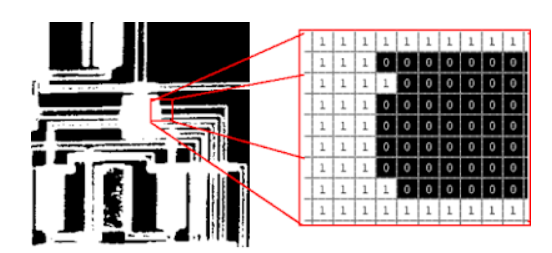
\includegraphics[width=\columnwidth]{Figures/insect2/binarynumber}
	\caption{ภาพแบบ Binary}{ที่มา: https://nextsoftwares.wordpress.com/2014/05/22/%E0%B8%84%E0%B8%A7%E0%B8%B2%E0%B8%A1%E0%B8%A3%E0%B8%B9%E0%B9%89%E0%B9%80%E0%B8%9A%E0%B8%B7%E0%B9%89%E0%B8%AD%E0%B8%87%E0%B8%95%E0%B9%89%E0%B8%99%E0%B9%80%E0%B8%81%E0%B8%B5%E0%B9%88%E0%B8%A2%E0%B8%A7/}
		\label{Fig:ิbinaryImage} 
	\end{figure}
	
	
	\begin{itemize}
		\item{Grayscale Image เป็นรูปที่เก็บโดยใช้รูปแบบของอาร์เรย์ 2 มิติ โดยค่าที่เก็บจะมีค่าอยู่ในช่วงๆหนึ่ง ซึ่งระดับของสีขึ้นอยู่กับขนาดของบิตที่ใช้เก็บค่าสี ดังรูปที่ \ref{Fig:ิGrayscaleImage}
		}
	\end{itemize}
	
	\begin{figure}[H]
		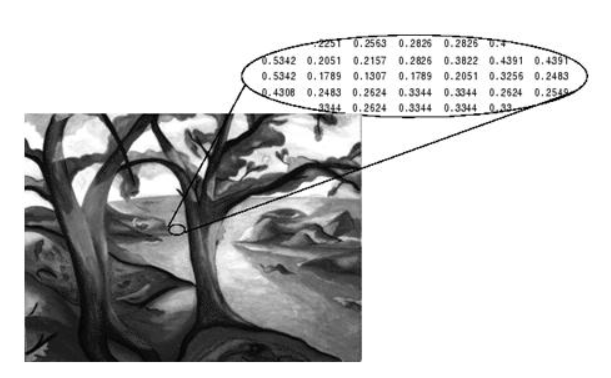
\includegraphics[width=\columnwidth]{Figures/insect2/GS}
		\caption{ภาพแบบ Grayscale Image}{ที่มา: https://nextsoftwares.wordpress.com/2014/05/22/%E0%B8%84%E0%B8%A7%E0%B8%B2%E0%B8%A1%E0%B8%A3%E0%B8%B9%E0%B9%89%E0%B9%80%E0%B8%9A%E0%B8%B7%E0%B9%89%E0%B8%AD%E0%B8%87%E0%B8%95%E0%B9%89%E0%B8%99%E0%B9%80%E0%B8%81%E0%B8%B5%E0%B9%88%E0%B8%A2%E0%B8%A7/}
			\label{Fig:ิGrayscaleImage} 
		\end{figure}
		
		\begin{itemize}
			\item{RGB Image หรือ Truecolor Image เป็นรูปที่เก็บโดยใช้อาร์เรย์ 3 มิติ ขนาด m x n x 3 โดยที่ m คือความยาว และ n คือความกว้างของภาพในหน่วยพิกเซล ส่วนมิติสุดท้ายนั้น ในแต่ละมิติจะเก็บค่าสีแยกกัน คือสีแดง (Red) สีเขียว (Green) และสีน้ำเงิน (Blue) ดังรูปที่ \ref{Fig:ิRGBImage}
			}
		\end{itemize}
		
		\begin{figure}[H]
			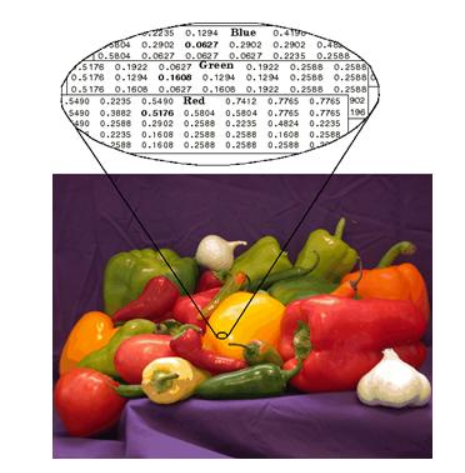
\includegraphics[width=\columnwidth]{Figures/insect2/RGB}
			\caption{ภาพแบบ RGB Image}{ที่มา: https://nextsoftwares.wordpress.com/2014/05/22/%E0%B8%84%E0%B8%A7%E0%B8%B2%E0%B8%A1%E0%B8%A3%E0%B8%B9%E0%B9%89%E0%B9%80%E0%B8%9A%E0%B8%B7%E0%B9%89%E0%B8%AD%E0%B8%87%E0%B8%95%E0%B9%89%E0%B8%99%E0%B9%80%E0%B8%81%E0%B8%B5%E0%B9%88%E0%B8%A2%E0%B8%A7/}
				\label{Fig:ิRGBImage} 
			\end{figure}
			\subsection{Machine Leaning}
			Machine Learning คือ ส่วนการเรียนรู้ของเครื่อง ถูกใช้งานเสมือนเป็นสมองของ AI (Artificial Intelligence) เราอาจพูดได้ว่า AI ใช้ Machine Learning ในการสร้างความฉลาด มักจะใช้เรียกโมเดลที่เกิดจากการเรียนรู้ของปัญญาประดิษฐ์ ไม่ได้เกิดจากการเขียนโดยใช้มนุษย์ มนุษย์มีหน้าที่เขียนโปรแกรมให้ AI 
			(เครื่อง) เรียนรู้จาก ข้อมูลเท่านั้น ที่เหลือเครื่องจัดการเอง Machine Learning เรียนรู้จากสิ่งที่เราส่งเข้าไปกระตุ้นแล้วจดจำเอาไว้เป็นมันสมอง ส่งผลลัพธ์ออกมาเป็นตัวเลข code หรือ ที่ส่งต่อไปแสดงผล หรือให้เจ้าตัว AI นำไปแสดงการกทำ Machine Learning เองสามารถเอาไปใช้งานได้หลายรูปแบบ ต้องอาศัยกลไกที่เป็นโปรแกรม หรือเรียกว่า Algorithm ที่มีหลากหลายแบบโดยมี Data Scientist เป็นผู้ออกแบบ หนึ่งใน Algorithm ที่ได้รับความนิยมสูง คือ DeepLearning ซึ่งถูกออกแบบมาให้ใช้งานได้ง่าย และประยุกต์ใช้ได้หลายลักษณะงาน อย่างไรก็ตาม ในการทำงานจริงของ Data Scientist จำเป็นต้องออกแบบตัวแปรต่างๆ ทั้งในตัวของ Deep Learning เองและต้องหา Algorithm อื่นๆ มาเป็นคู่เปรียบเทียบ เพื่อมองหา Algorithm ที่เหมาะสมที่สุดในการใช้งานจริง
			
			Algorithm ที่นำมาใช้ในการวิเคราะห์ ในส่วนของฟังก์ชันคือกฎความสัมพันธ์(Associations) การทำเหมืองข้อมูลเพื่อหาความสัมพันธ์ของเหมืองข้อมูลมักใช้ในธุรกิจการค้าปลีก(retailing Business) เช่น ร้านค้าสะดวกซื้อ หรือ ซุปเปอร์มาเก็ต เป็นการวิเคราะห์การตลาด(Marketing basket Analysis) เพื่อศึกษาพฤติกรรมการซื้อสินค้าของลูกค้า และหาความสัมพันธ์ของสินค้าที่ลูกค้าซื้อ
			
			ความสัมพันธ์ของสินค้าที่ลูกค้าซื้อจะแสดงในรูปของกฎความสัมพันธ์  Association Rule ดังนี้
			
			\begin{figure}[H]
				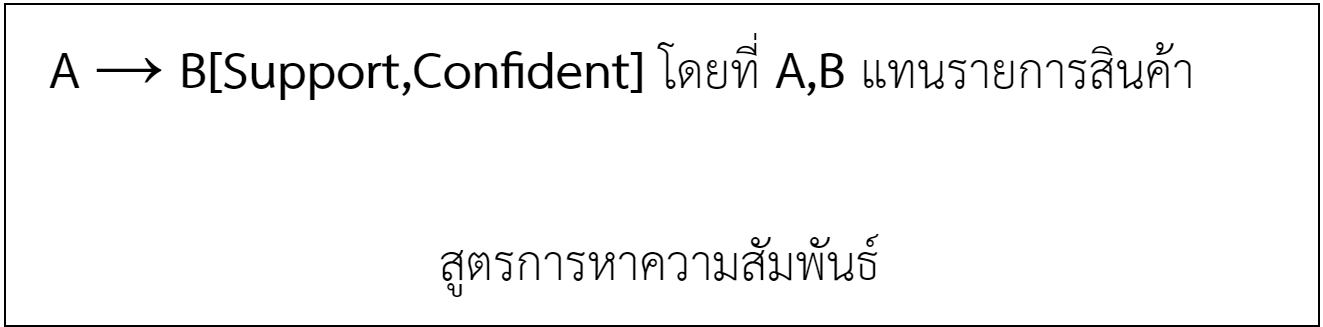
\includegraphics[width=\columnwidth]{Figures/insect2/AS}
				\caption{สูตรการหาความสัมพันธ์ Association Rule}
				\label{Fig:AS} 
			\end{figure}
		
			 
			 \newline
			 เช่น Milk -> Eggs [Support = 25 เปอร์เซ็น ,Confident=33.34 เปอร์เซ็น] หมายความว่า 25เปอร์เซ็น ของทรานแซคชั่นทั้งหมด ลูกค้า จะซื้อนม (Milk) และซื้อไข่ (Eggs) พร้อมกันและ 33.34 เปอร์เซ็น ของลูกค้าที่ซื้อนมแล้วจะซื้อไข่ด้วย กฎความสัมพันธ์ที่สนใจหรือกฎความสัมพันธ์ที่แข็งแกร่ง (Strong Association Rules) คือ กฎความสัมพันธ์ที่มีค่าสนับสนุน (support) และค่าความเชื่อมั่น (confidence) ผ่านเกณฑ์ขั้นต่ำ(Minimum Threshold) ที่ผู้วิเคราะห์ข้อกำหนดขึ้นมา
			  
			  
	     	\end{figure}
			\section{ความรู้พื้นฐานเกี่ยวกับ Pillow}
			Pillow  เป็น  Library ด้านความสามารถในการประมวลผลภาพและกราฟฟิก หรือโมดูลจัดการและประมวลผลรูปภาพบน Python ใน Python มีโมดูลด้านที่ชื่อว่า Python Imaging Library (PIL) ซึ่งรองรับแต่ Python 2  จึงมีคนมาพัฒนาเป็นโมดูล Pillow  ที่รองรับทั้ง Python 2 และ Python 3  โมดูล Pillow สามารถจักการจัดเก็บรูปภาพ (Image Archives) แสดงรูปภาพ (Image Display) ประมวลผลรูปภาพ เช่น ปรับขนาดรูปภาพ แปลงไฟล์รูปภาพ ใส่ตัวอักษรลงในภาพ และอื่น ๆ เป็นต้น ดังรูปที่ \ref{Fig:pillow}
			
			\begin{figure}[H]
				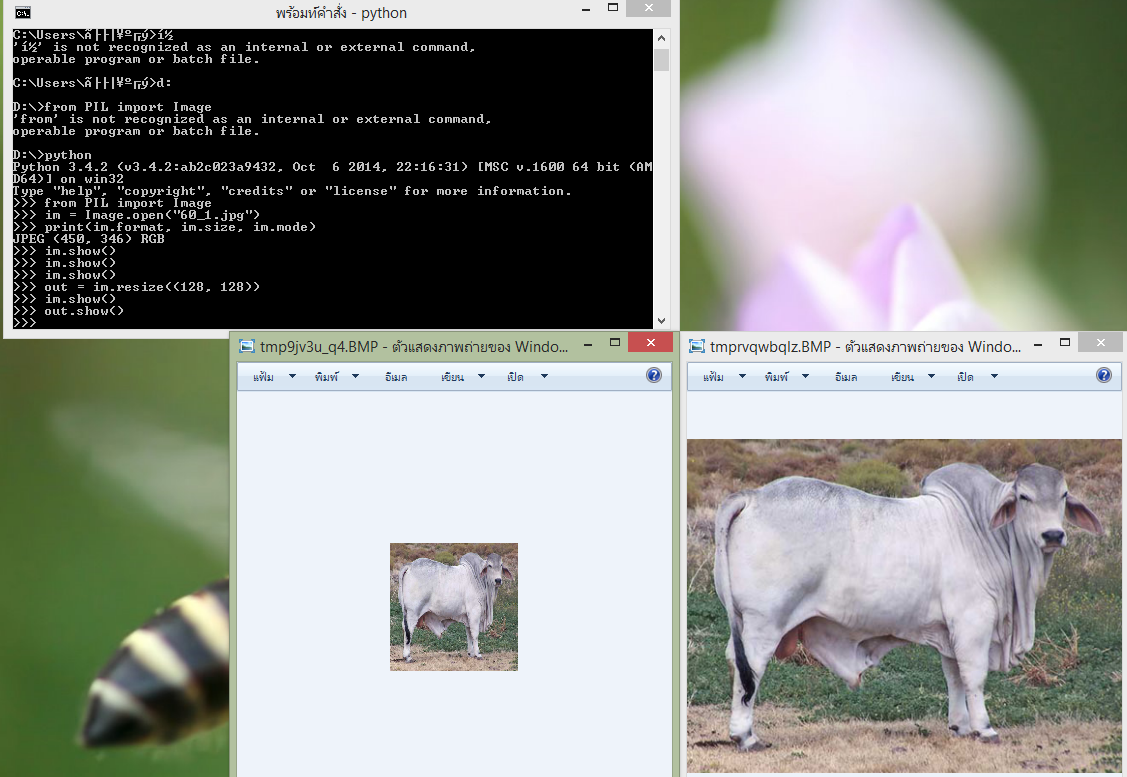
\includegraphics[width=\columnwidth]{Figures/insect2/pillow}
				\caption{การขยายรูปโดยใช้ Pillow}{ที่มา: https://python3.wannaphong.com/2014/11/image-processing-python.html}
				\label{Fig:pillow} 
			\end{figure}
		\section{MySQL}
		MySQL  คือ โปรแกรมระบบจัดการฐานข้อมูล ที่พัฒนาโดยบริษัท MySQL AB มีหน้าที่เก็บข้อมูลอย่างเป็นระบบ รองรับคำสั่ง SQL เป็นเครื่องมือสำหรับเก็บข้อมูลที่ต้องใช้ร่วมกับเครื่องมือหรือโปรแกรมอื่นอย่างผสมผสาน เพื่อให้ได้ระบบงานที่รองรับความต้องการของผู้ใช้ เช่น ทำงานร่วมกับเครื่องบริการเว็บ (Web Server) เพื่อให้บริการแก่ภาษาสคริปต์ที่ทำงานฝั่งเครื่องบริการ Server-Side Script เช่น ภาษา PHP ภาษา ASP.NET หรือภาษา JSP เป็นต้น หรือทำงานร่วมกับโปรแกรมประยุกต์ (Application Program) เช่น ภาษาวิชวลเบสิกดอทเน็ต (Visual Basic.NET) ภาษาจาวา (JAVA) หรือภาษาซีชาร์ป (C\#) เป็นต้น โปรแกรมถูกออกแบบให้สามารถทำงานได้บนระบบปฏิบัติการที่หลากหลาย และเป็นระบบฐานข้อมูลโอเพนซอร์ส (Open Source) ที่ถูกนำไปใช้งานมากที่สุด
		
		ความสามารถและการทำงานของโปรแกรม MySQL มีดังต่อไปนี้ 
		
		\begin{itemize}
			\item{MySQL (DataBase Management System : DBMS) 
				เป็นฐานข้อมูลที่มีลักษณะเป็นโครงสร้างของการเก็บรวบรวมข้อมูล การที่จะเพิ่ม เข้าถึงหรือประมวลผลข้อมูลที่เก็บในฐานข้อมูลจำเป็นจะต้องอาศัยระบบจัดการฐานข้อมูล ซึ่งจะทำหน้าที่เป็นตัวกลางในการจัดการกับข้อมูลในฐานข้อมูลทั้งสำหรับการใช้งานเฉพาะ และรองรับการทำงานของแอปพลิเคชันอื่นๆ ที่ต้องการใช้งานข้อมูลในฐานข้อมูล เพื่อให้ได้รับความสะดวกในการจัดการกับข้อมูลจำนวนมาก MySQL ทำหน้าที่เป็นทั้งตัวฐานข้อมูลและระบบจัดการฐานข้อมูล}
			\item{MySQL เป็นระบบจัดการฐานข้อมูลแบบ relational 
				ซึ่งฐานข้อมูลแบบ relational จะทำการเก็บข้อมูลทั้งหมดในรูปแบบของตารางแทนการเก็บข้อมูลทั้งหมดลงในไฟล์ เพียงไฟล์เดียว ทำให้ทำงานได้รวดเร็วและมีความยืดหยุ่น นอกจากนั้น แต่ละตารางที่เก็บข้อมูลสามารถเชื่อมโยงเข้าหากันทำให้สามารถรวมหรือจัดกลุ่มข้อมูลได้ตามต้องการ โดยอาศัยภาษา SQL ที่เป็นส่วนหนึ่งของโปรแกรม MySQL ซึ่งเป็นภาษามาตรฐานในการเข้าถึงฐานข้อมูล}
			\item{MySQL แจกจ่ายให้ใช้งานแบบ Open Source คือ ผู้ใช้งาน MySQL ทุกคนสามารถใช้งานและปรับแต่งการทำงานได้ตามต้องการ สามารถดาวน์โหลดโปรแกรม MySQL ได้จากอินเทอร์เน็ต (Internet) และนำมาใช้งานโดยไม่มีค่าใช้จ่าย}
		\end{itemize}
		
		\section{XAMPP}
		การพัฒนาเว็บไซต์ หรือโปรแกรมที่ทำงานบนเว็บแอปพลิเคชัน จำเป็นต้องอาศัยเครื่องแม่ข่ายเว็บ (Web server) ซึ่งอาจจะเป็นภาระสำหรับผู้เรียน หรือผู้พัฒนาบางกลุ่ม แนวทางหนึ่งที่นิยมกันคือ การจำลองเครื่องพีซีให้เป็นเครื่องแม่ข่ายเว็บด้วยโปรแกรมสำเร็จรูป ซึ่งมีให้เลือกหลายค่ายซึ่ง
		XAMPP เป็นหนึ่งในผลิตภัณฑ์ที่มีการพัฒนาออกมาให้ใช้งาน
		
		XAMPP  พัฒนาโดยโครงการ Apache Friends ที่เป็นโครงการไม่แสวงหาผลกำไร ที่จัดตั้งในปี ค.ศ. 2002 โดย Kai ‘Oswald’ Seidler และ Kay Vogelgesang ทั้งนี้ XAMPP ประกอบด้วยโปรแกรมย่อยได้แก่ โปรแกรม Apache โปรแกรมฐานข้อมูล MySQL โปรแกรมภาษา PHP และภาษา Perl อีกทั้ง XAMPP มีการปรับปรุงรุ่นอย่างต่อเนื่องเพื่อให้ทำงานได้กับระบบปฏิบัติการทั้ง Microsoft Windows, Mac OS x, Linux และ Solaris นอกจากนี้ยังไม่มีค่าใช้จ่ายในการดาวน์โหลดใช้งาน
		
		แนวคิดของ XAMPP
		
		XAMPP โปรแกรมรวมการติดตั้งสำหรับนักพัฒนาโปรแกรมของ Apache เพื่อที่ให้โปรแกรมนั้นใช้งานง่ายและสะดวกสำหรับนักพัฒนาโปรแกรม โปรแกรม XAMPP นั้นได้ตั้งค่าเริ่มต้น ให้สามารถใช้งานโปรแกรม XAMPP แบบใช้งานโปรแกรมได้ในทุกอย่าง (all features turn on)
		ค่ามาตรฐานนี้ อาจจะเป็นจุดอ่อนในเรื่องความปลอดภัย หากนำไปใช้ในเครื่องที่ใช้งานจริง เพราะโปรแกรม XAMPP ถูกออกแบบมาสำหรับเครื่องของนักพัฒนาโปรแกรม
		
		ประโยชน์ของ XAMPP
		\begin{itemize}
			\item สะดวกในการติดตั้งและถอนการติดตั้ง
			\item โปรแกรมมีคำสั่งต่างๆ ทำให้ง่ายต่อการใช้งาน
			\item โปรแกรมสามารถใช้งานได้ในหลายระบบปฏิบัติการ เช่น  Linux, Windows, Mac OSX หรือ ระบบปฏิบัติการอื่นๆ
			\item เป็นโปรแกรมฟรีที่สนับสนุนในการใช้งานของผู้ที่ต้องการพัฒนาระบบ 
		\end{itemize}
		
			
			\section{ความรู้พื้นฐานเกี่ยวกับปัญญาประดิษฐ์ (Artificial Intelligence)}
			ปัญญาประดิษฐ์ (AI) เป็นศาสตร์แขนงหนึ่งของวิทยาศาสตร์ คอมพิวเตอร์ ที่เกี่ยวข้องกับวิธีการทำให้คอมพิวเตอร์มีความสามารถคล้ายมนุษย์ หรือเลียนแบบพฤติกรรมมนุษย์ โดยเฉพาะความสามารถในการคิดเองได้ หรือมีปัญญานั่นเอง ปัญญานี้มนุษย์เป็นผู้สร้างให้คอมพิวเตอร์ จึงเรียกว่าปัญญาประดิษฐ์  
			
			\subsection{โครงข่ายประสาทเทียม (Neural Network) }
			โครงข่ายประสาทเทียม  คือ โครงข่ายประสาทเทียมที่เป็นการจำลองมาจากสมองของมนุษย์ เพื่อจำลองการทำงานของเครือข่ายประสาทในสมองมนุษย์ ด้วยวัตถุประสงค์ที่จะสร้างเครื่องมือ ซึ่งมีความสามารถในการเรียนรู้การจดจำรูปแบบ (Pattern Recognition) และการสร้างความรู้ใหม่ (Knowledge Extraction) เช่นเดียวกับความสามารถที่มีในสมองมนุษย์นั่นเอง
			หลักการของ Neural Network 
			ในคอมพิวเตอร์ neurons ประกอบด้วย input และ output เหมือนกัน โดยจำลองให้ input แต่ละอันมี weight เป็นตัวกำหนดน้ำหนักของ input โดย neuron แต่ละหน่วยจะมีค่า threshold เป็นตัวกำหนดว่าน้ำหนักรวมของ input ต้องมากขนาดไหนจึงจะสามารถส่ง output ไปยัง neurons ตัวอื่นได้ เมื่อนำ neuron แต่ละหน่วยมาต่อกันให้ทำงานร่วมกันการทำงานนี้ในทางตรรกแล้ว จะเหมือนกับปฏิกิริยาเคมีที่เกิดในสมอง เพียงแต่ในคอมพิวเตอร์ทุกอย่างเป็นตัวเลขเท่านั้นเอง ดังรูปที่ \ref{Fig:CNN}
			\begin{figure}[H]
				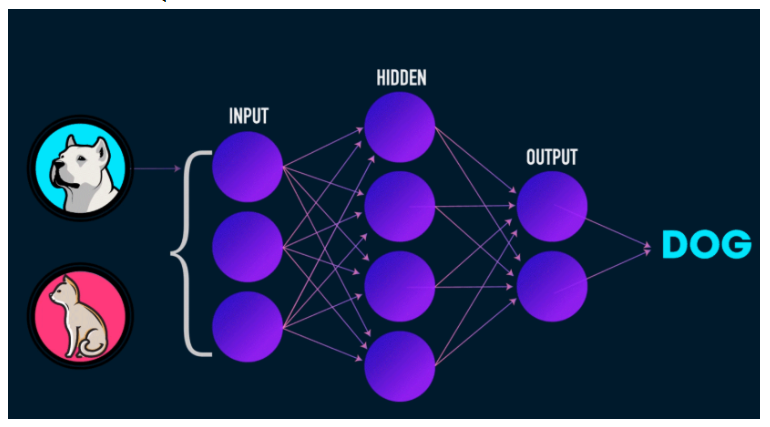
\includegraphics[width=\columnwidth]{Figures/insect2/NN}
				\caption{ขั้นตอนของโครงข่ายประสาทเทียมแบบคอนโวลูชันนัล}{ที่มา: https://analyticsindiamag.com/most-common-activation-functions-in-neural-networks-and-rationale-behind-it/}
				\label{Fig:CNN} 
			\end{figure}

          \section{งานวิจัยที่เกี่ยวข้อง}
          นางสาวสุภาภรณ์ จินดาวงษ์ ได้นำเสนอวิจัยเกี่ยวกับ การศึกษาพฤติกรรมการเลอืกใช้บริการร้านกาแฟสดของผู้บริโภค ผู้ศึกษาจึงสนใจเกี่ยวกับ พฤติกรรมการเลือกใช้บริการร้านกาแฟสดของผู้บริ โภคในอำเภอเมือง จังหวัด นครปฐม กรณีศึกษา ร้านบ้านไร่กาแฟ สาขาที่29 เพื่อทราบถึงเหตุผลการเข้าใช้บริการร้านกาแฟสดบ้านไร่กาแฟ สาขาที่29 ผลการวิจัยทำให้
          สามารถใช้เป็นแนวทางในการปรับปรุงธุรกิจให้ตรงกับความตอ้งการผู้บริโภคและเป็นแนวทาง
          ดำเนินกิจการแก่ผู้สนใจธุรกิจร้านกาแฟ
		  
		  	
		  นางสาวกานดา เสือจำศิล ได้นำเสนอวิจัยเกี่ยวกับ พฤติกรรมการเข้าใช้บริการร้านกาแฟสด อเมซอน ของผู้บริโค เพื่อศึกษาพฤติกรรมการเข้าใช้บริการร้านกาแฟสด อเมซอน ปัจจัยส่วนบุคคลของผู้บริโภคที่เข้าใช้บริการร้านกาแฟสด อเมซอน และปัจจัยส่วนผสมทางการตลาดต่อการเข้าใช้บริการร้านกาแฟสด อเมซอน กลุ่มตัวอย่างที่ใช้ คือ ผู้บริโภคในจังหวัดปทุมธานีที่เข้าใช้บริการร้านกาแฟสด อเมซอน จำนวน 400 คน
		  \newline
		  	

	

\chapter{การวิเคราะห์และออกแบบระบบ}

การวิเคราะห์และออกแบบระบบก่อนดำเนินการจริงเป็นอีกหนึ่งขั้นตอนที่มีความสำคัญมาก เพราะการวิเคราะห์และออกแบบระบบนั้นเป็นการกระทำที่ทำให้ผู้พัฒนาเห็นรายละเอียดส่วนย่อยของงานทั้งหมด เพิ่มประสิทธิภาพในการวางแผน การทำงาน และยังช่วยลดปัญหาที่อาจจะเกิดขึ้นในระหว่างพัฒนา เพื่อให้ระบบมีความสมบูรณ์มากยิ่งขึ้น เนื่องจากการวิเคราะห์และออกแบบระบบนั้นจะช่วยให้ให้บริการ จัดการทรัพยากรได้อย่างคุ้มค่าและตรงตามความต้องการของระบบ

การวิเคราะห์และออกแบบระบบสแกนใบหน้าสำหรับเเคชเชียร์ ในบทนี้จะแบ่งออกเป็น 6 ข้นตอนเพื่อให้เห็นการดำเนินงานอย่างมีระบบ ในหัวข้อแรกจะนำเสนอภาพรวมของระบบ ก่อนจะนำเสนอเอกสารแสดงความต้องการของระบบซึ่งจะทำให้เห็นที่มาของเพจต่าง ๆ ในขั้นตอนของการออกแบบในหัวข้อที่สาม ส่วนหัวข้อที่เหลือจะแสดงแผนภาพการการทำงานของระบบโดยใช้ UML diagram ซึ่งประกอบไปด้วย Use Case, Class และ Sequence Diagram เพื่อแสดงรายละเอียดของระบบก่อนนำไปเขียนคำสั่งด้วยภาษาโปรแกรมในบทต่อไป

\begin{enumerate}[label=3.\arabic*]
	\item โครงสร้างภาพรวมของระบบ (System Architecture) เป็นการออกแบบภาพรวมและเทคโนโลยีของระบบ	
	\item System Requirements คือ ความต้องการหรือสิ่งที่ระบบควรจะทำ หรือหน้าที่หลักของ
	ระบบที่จะต้องทำ
	\item User Interface Design เป็นการออกแบบส่วนต่อประสานกับผู้ใช้
	\item Use Case Diagram เป็นแผนภาพที่ใช้แสดงให้ทราบว่าระบบทำงานหรือมีหน้าที่ใดบ้าง
	\item Class Diagram เป็นแผนภาพที่ใช้แสดง Class และความสัมพันธ์ระหว่าง Class
	\item Sequence Diagram เป็นแผนภาพที่ใช้แสดงให้เห็นถึงการตอบโต้ข้อมูลระหว่างคลาส เรียงตามลำดับของเวลาที่เกิดเหตุการณ์จากน้อยไปมาก
\end{enumerate}	

\section{โครงสร้างภาพรวมของระบบ}
    ความหมายของ System Architecture  หมายถึง กรอบโครงสร้างของระบบที่อธิบายความสัมพันธ์ขององค์ประกอบต่าง ๆ ไปจนถึงขั้นการเชื่อมต่อกันของระบบย่อยต่าง ๆ โดยจัดกลุ่มองค์ประกอบไว้ในหลาย ๆ ลักษณะเพื่อให้ผู้เกี่ยวข้อง (Stakeholder) จากพื้นฐานสาขาอาชีพที่แตกต่าง กันสามารถทำความเข้าใจได้ง่าย เช่น การจัดแบ่งองค์ประกอบตามลักษณะการทำงานของระบบ (functional components) เป็นต้น
    
    การออกแบบ System architecture แสดงภาพรวมและเทคโนโลยีของระบบสแกนใบหน้าสำหรับเเคชเชียร์ มีรายละเอียดดังรูปที่ \ref{Fig:system}
   
  \begin{figure}[H]
  	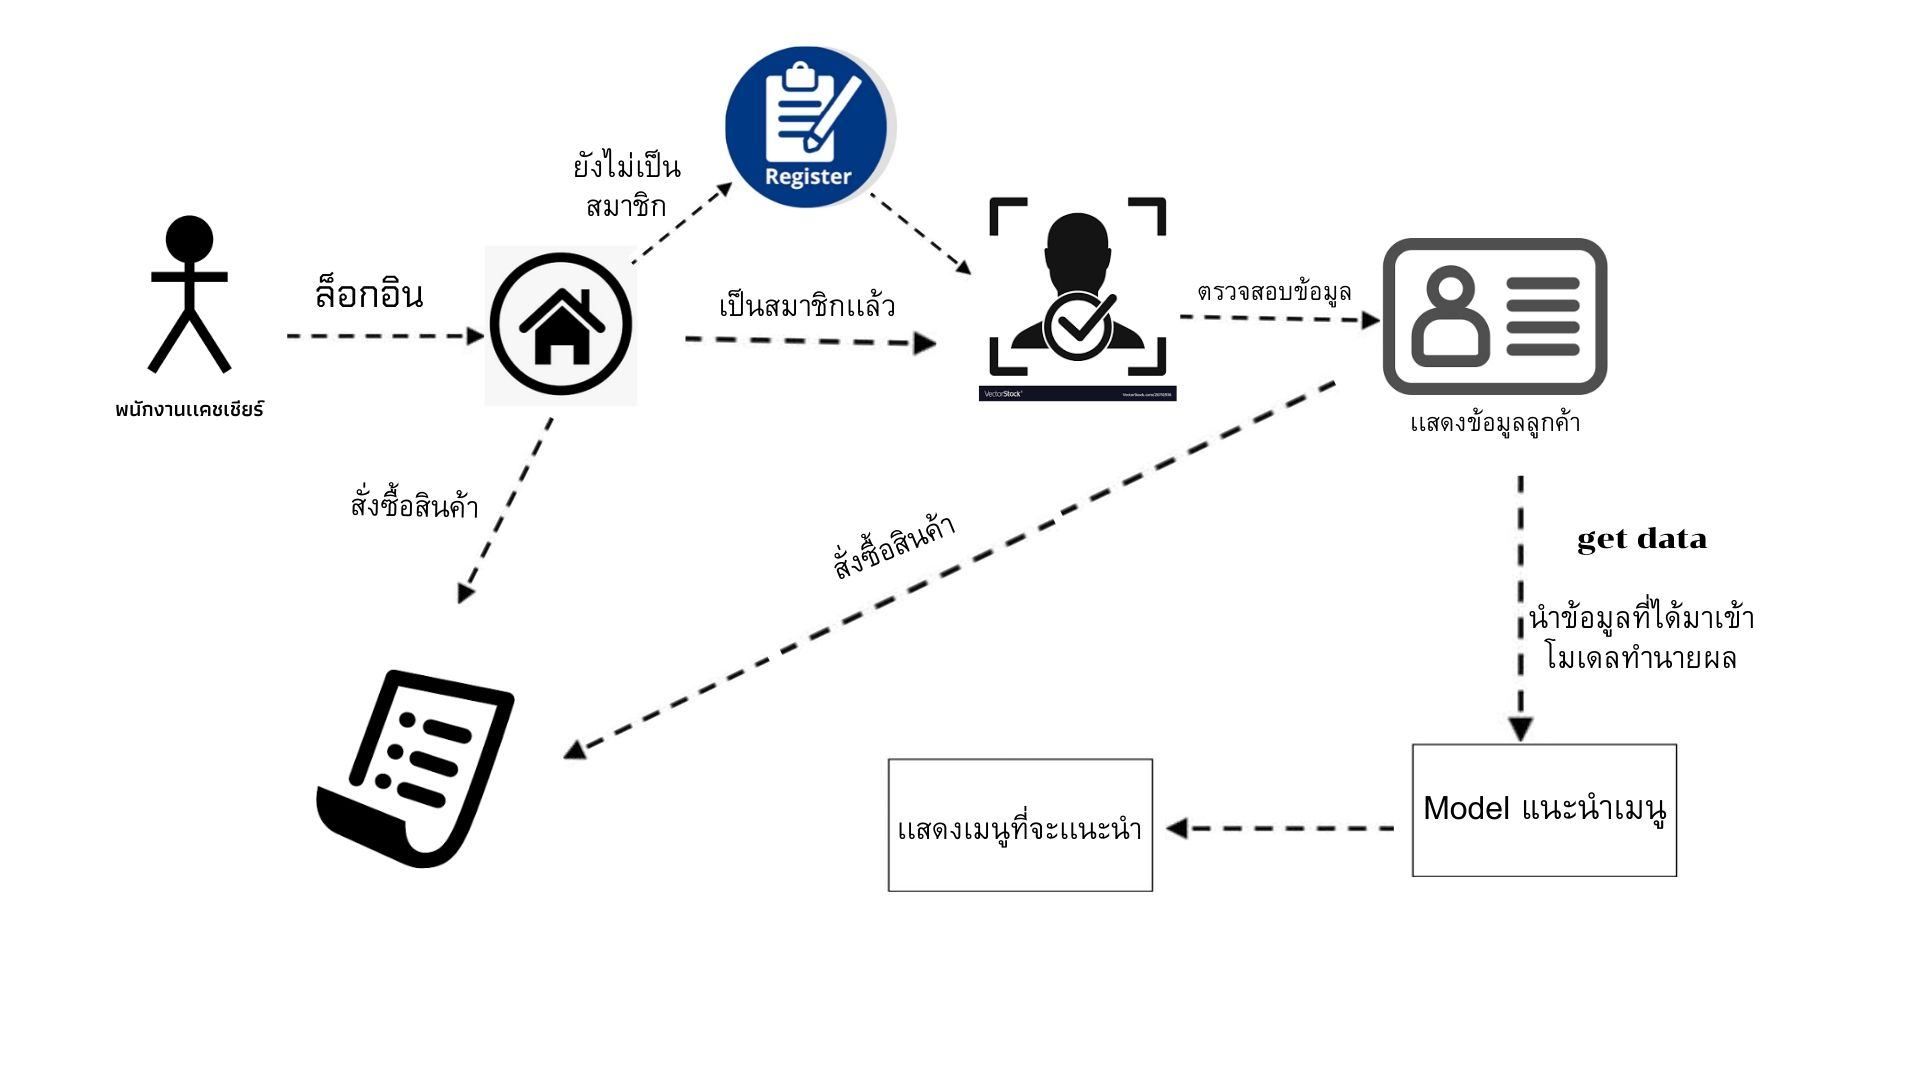
\includegraphics[width=\columnwidth]{Figures/chapter3/system}
  	\caption{ภาพรวมและโครงสร้างการทำงานของระบบ}
  	\label{Fig:system} 
  \end{figure}
   
   จากรูปที่ \ref{Fig:system}เมื่อพนักงานเเคชเชียร์ทำการล็อกอินเเล้วจะเข้าหน้าหลัก ยังไม่เป็นสมาชิกจะทำการสมัครก่อน ถ้าเป็นสมาชิกเเล้วจะเข้าสู่สู่ระบบสแกนใบหน้าสำหรับลูกค้า โดยระบบจะทำการตรวจสอบรูปภาพที่สแกนว่าตรงกับรูปภาพของในระบบ แล้วเเสดงจ้อมูลของลูกค้าให้กับพนักงานเเคชเชียร์แล้วยังหน้าสั่งสินค้า หรือต้องการใช้ระบบเเนะนำเมนูแก่ลูค้าระบบจะทำการดึงข้อมูลไปให้โมเดลทำนาย เเล้วจะเเสดงเมนูที่จะเเนะนำให้ลูกค้าเเล้วทำการสั่งสินค้า
  

\section{System Requirements}
\subsection{Functional Requirements}
	ระบบสแกนใบหน้าสำหรับเเคชเชียร์ แบ่งความสามารถของระบบตามประเภทของผู้ใช้งานดังนี้
	\begin{enumerate}
		\item พนักงานเเคชเชียร์
			\begin{itemize}[label={--}]
				\item สามารถทำการเข้าสู่ระบบได้
				\item สแกนใบหน้าของลูกค้าได้
				\item สมัครสมาชิกให้ลูกค้าได้
				\item แก้ไขข้อมูลลูกค้าเมื่อลูกค้าต้องการได้
				\item สามารถเเนะนำเมนูเเก่ลูกค้าได้
				\item สามารถสั่งสินค้าให้ลูกค้าได้
				
			\end{itemize}
		\item ลูกค้า
			\begin{itemize}[label={--}]
				\item สแกนใบหน้าเพื่อทำการเเสดงข้อมูล
				\item สั่งสินค้ากับพนักงาน
			
			\end{itemize}
	\end{enumerate}

\subsection{Non-functional Requirements}
		\begin{enumerate}
		\item เว็บแอปพลิเคชัน
		\begin{itemize}[label={--}]
			\item ใช้โปรโตคอล (Protocol) แบบ HTTPS (Hypertext Transfer Protocol Secure)  ในการสื่อสารที่ช่วยรักษาความสมบูรณ์ถูกต้องของข้อมูลผู้ใช้และเก็บข้อมูลไว้เป็นความลับระหว่างคอมพิวเตอร์ของผู้ใช้กับเว็บไซต์ 
			\item ใช้ดีลิบ (dlib)ซึ่งมี Machine learning algorithms  ในการจดจำหน้าของลูกค้าเพือระบุตัวตน
			\item  ใช้ต้นไม้ตัดสินใจ (Decision Trees)
			ในการทำโมเดล(Model) ในการทำระบบเเนะนำเมนู
	\end{enumerate}
	
\section{User Interface Design}
ในการออกแบบ User Interface Design ของระบบสแกนใบหน้าสำหรับเเคชเชียร์
	
			\begin{itemize}
				
					\item  การออกแบบหน้าจอเข้าสู่ระบบ
				\begin{figure}[H]
					\centering
					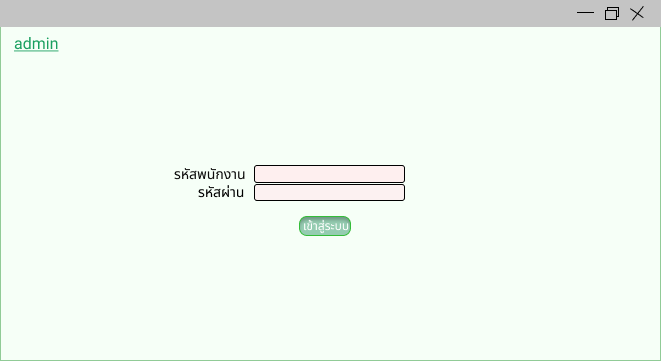
\includegraphics[width=0.8\textwidth]{Figures/3/UIWeb/login}
					\caption{หน้าเข้าสู่ระบบสำหรับพนักงาน}
					\label{Fig:login}
				\end{figure}
				จากภาพที่ \ref{Fig:login}  แสดงหน้าจอการเข้าสู่ระบบของพนักงานเเคชเชียร์ จำเป็นต้องกรอกข้อมูรหัสพนักงานและรหัสผ่านเพื่อเข้าใช้งานระบบ
				\en
				\item การออกแบบหน้าจอหลัก
				\begin{figure}[H]
					\centering
					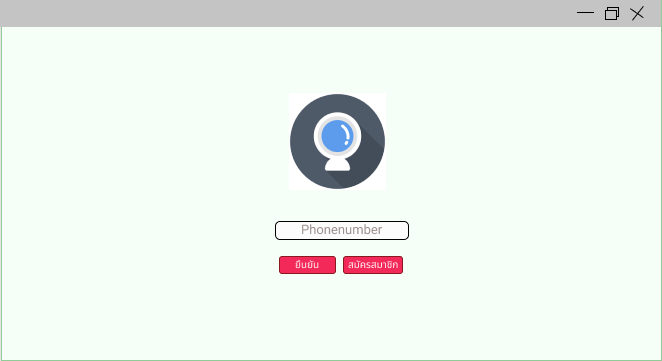
\includegraphics[width=0.8\textwidth]{Figures/3/UIWeb/Homepage}
					\caption{หน้าจอหลัก}
					\label{Fig:Homepage}
				\end{figure}
				จากภาพที่ \ref{Fig:Homepage}แสดงหน้าจอหลัก ให้พนักงานเลือก
				ไหยังหน้า สมัครสมาชิก เข้าสู่ระบบโดยการสแกนใบหน้า ดขเาสู่ระบบโดยล็อกอินผ่านเบอร์โทรศัพท์ 
				
				\begin{figure}[H]
					\centering
					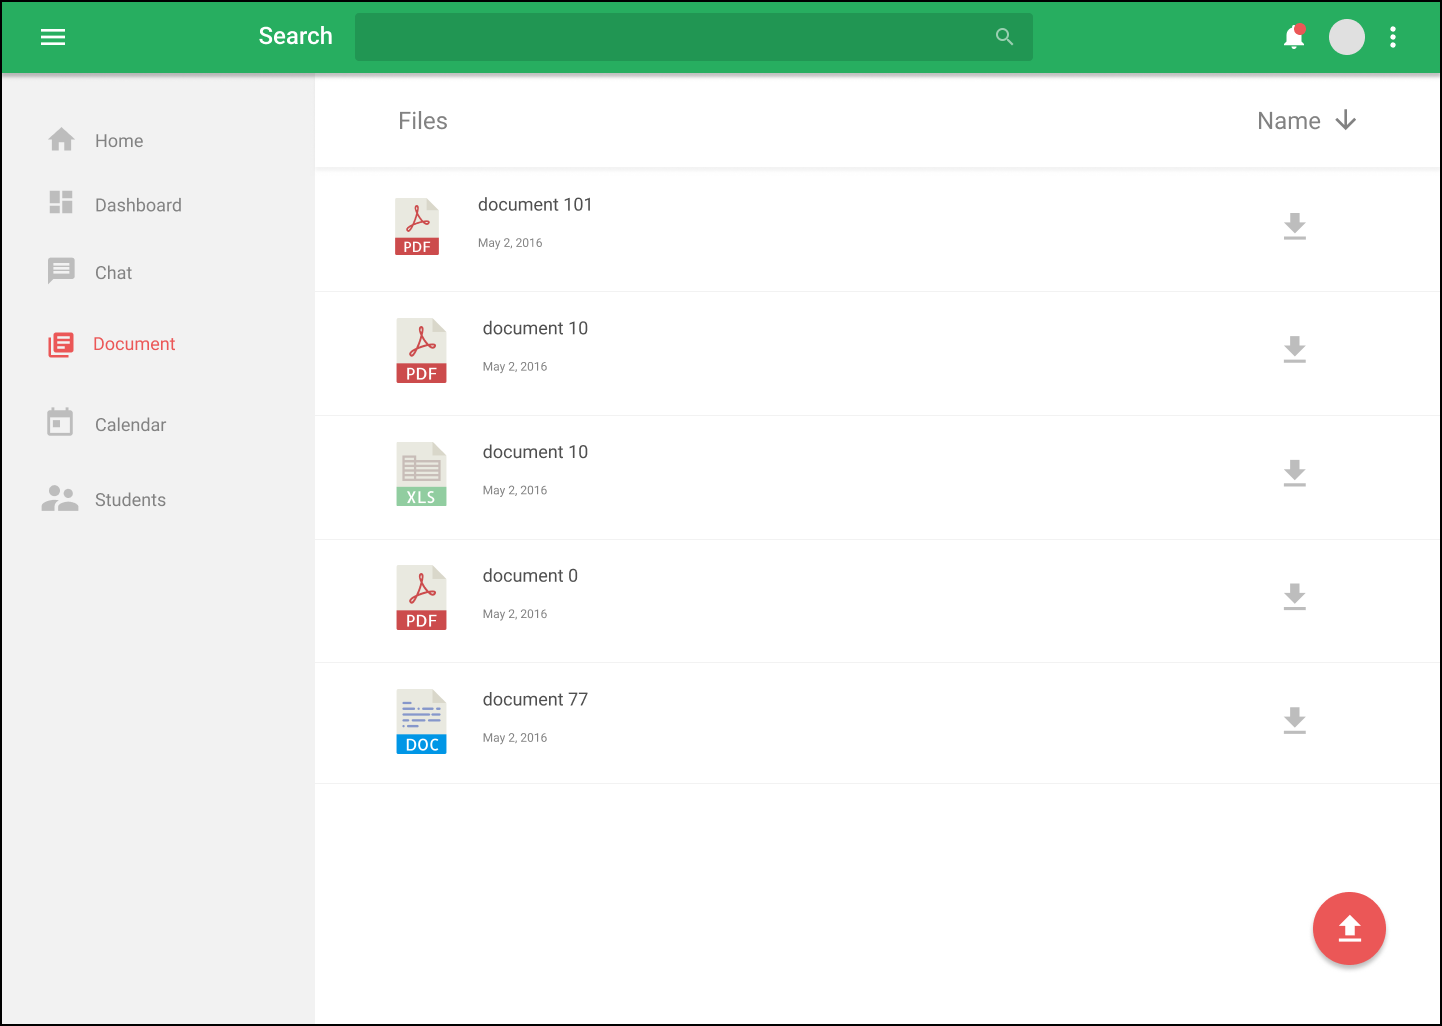
\includegraphics[width=0.8\textwidth]{Figures/3/UIWeb/Doc}
					\caption{หน้าจเเสดงข้อมูลลูกค้า}
					\label{Fig:Doc}
				\end{figure}
				จากภาพที่ \ref{Fig:Doc}  แสดงหน้าจอ ข้อมูลลูกค้า หลังจากที่ผ่านการสแกนใบหน้า จะเเสดงข้อมูลลูกค้าที่สมัครสมาชิก เเสดงประวัติการสั่งซื้อสินค้า แต้มสะสม เเละมีการกนะนำเมนูแก่ลูกค้า ทั้งนี้จะเเสดงเฉพาะลูกค้าที่เป็นสมาชิกเท่านั้น
				\item การออกเเบบหน้าจอสั่งซื้อสินค้า
				\begin{figure}[H]
					\centering
					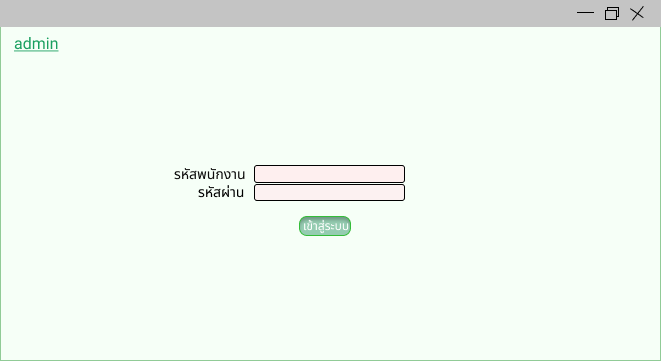
\includegraphics[width=0.8\textwidth]{Figures/3/UIWeb/Login}
					\caption{หน้าจอสั่งซื้อสินค้า}
					\label{Fig:Login}
				\end{figure}
				จากภาพที่ \ref{Fig:Login} แสดงหน้าจอรายการเมนูที่มีในร้าน โดยจะมีอยู่3ประเภทหลัก คือ เมนูร้อน เมนูเย็น เมนูปั่น เมื่อลูกค้าสั่งจะมีการเเสดงรายการที่สั่ง ราคา จำนวนที่ลูกค้าสั่ง
			\end{itemize}
	\newpage

\section{Use Case Diagram}
Use Case Diagram เป็นแผนผังเพื่อแสดงฟังก์ชันแสดงการทำงานของระบบโดยรวม แสดงส่วนประกอบในระบบและกิจกรรมที่เกิดขึ้นในระบบ สัญลักษณ์ที่ใช้ในการเขียน Use Case Diagram แสดงในตารางที่ \ref{tab:use-case2}
\begin{table}[H]
	\caption{สัญลักษณ์ของ Use case Diagram}
	\label{tab:use-case2}
	\begin{tabular}{|c|p{10cm}|}
		\hline
		\textbf{สัญลักษณ์} & \multicolumn{1}{c|}{\textbf{การใช้งาน}} \\ \hline
		\raisebox{-\totalheight}{Use case}
		& \setstretch{1.5} {Use case คือส่วนย่อยของระบบงาน แทนด้วยวงรีและชื่อของ Use case ภายในวงรี} \\ \hline
		\raisebox{-\totalheight}{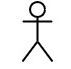
\includegraphics[height=1.5cm]{Figures/table/use-case/2}}
		& \setstretch{1.5} {Actor คือบุคคลหรือระบบงานอื่นที่ใช้งานระบบหรือได้รับประโยชน์จากระบบซึ่งอยู่ภายนอกระบบ แทนด้วยรูปคนและมีชื่อบทบาทการใช้งานระบบ} \\ \hline
		\raisebox{-\totalheight}{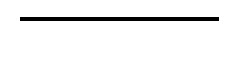
\includegraphics[width=3cm]{Figures/table/use-case/3}}
		& \setstretch{1.5} {เส้นตรงที่แสดงถึงการใช้งาน Use case ของผู้กระทำ} \\ \hline
		\raisebox{-\totalheight}{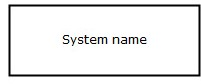
\includegraphics[width=0.3\textwidth]{Figures/table/use-case/4}}
		& \setstretch{1.5} {กรอบสี่เหลี่ยมแสดงถึงขอบเขตของระบบโดยแสดงชื่อระบบภายในหรือด้านบนกรอกสี่เหลี่ยม Use case อยู่ภายในกรอบสี่เหลี่ยม และ actor อยู่ภายนอกกรอบสี่เหลี่ยม} \\ \hline
		\raisebox{-\totalheight}{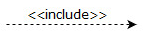
\includegraphics[width=0.3\textwidth]{Figures/table/use-case/5}}
		& \setstretch{1.5} {ความสัมพันธ์แบบ <<includes>> แสดงว่า Use case หนึ่งดำเนินการตามขั้นตอนของ Use case อื่น โดยแทนด้วยสัณลักษณ์ลูกศรเส้นประ ซึ่ง Use case ที่หางลูกศรเรียกใช้งาน Use case ที่หัวลูกศรทุกครั้งที่มีการทำงาน} \\ \hline
		\raisebox{-\totalheight}{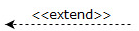
\includegraphics[width=0.3\textwidth]{Figures/table/use-case/6}}
		& \setstretch{1.5} {ความสัมพันธ์แบบ <<extend>> แสดงว่า Use case หนึ่งดำเนินการตามขั้นตอนของ Use case อื่น โดยแทนด้วยสัญลักษณ์ลูกศรเส้นประ ซึ่ง Use case ที่หัวลูกศรเรียกใช้งาน Use case ที่หางลูกศร แต่การใช้งานไม่จำเป็นต้องเกิดขึ้นทุกครั้งขึ้นอยู่กับเงื่อนไขระหว่างการทำงาน} \\ \hline
	\end{tabular}
\end{table}


	 \begin{figure}[H]
		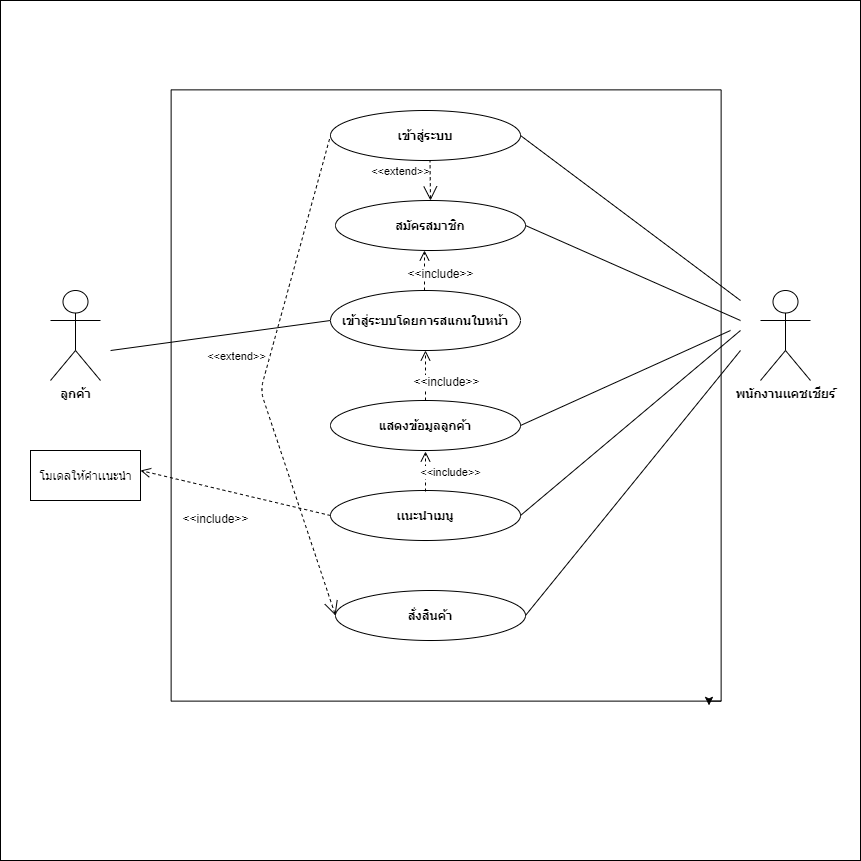
\includegraphics[width=\columnwidth]{Figures/3/usecase}
		\caption{Use Case diagram ของระบบ สแกนใบหน้าสำหรับเเคชเชียร์}
		\label{Fig:usecase} 
	\end{figure}
	
	\begin{table}[H]
		\centering
		\caption{อธิบาย Use Case หน้าที่ของระบบ ในภาพที่ \ref{Fig:usecase}}
		\label{tab:usecase}
		\resizebox{\totalheight}{!}{\textwidth}{%
			\begin{tabular}{|c|p{10cm}|}
				\hline
				\multicolumn{1}{|c|}{\textbf{Use Case}} & \multicolumn{1}{c|}{\textbf{คำอธิบาย}} \\ \hline
		สมัครสมาชิก & พนักงานทำการสมัครสมาชิกแก่ลูกค้าที่ต้องการเป็นสมาชิกโดยผ่านการล็อกอินของพนักงานก่อน\\ \hline
					สแกนใบหน้าลูกค้า & พนักงานสแกนใบหน้าลุกค้าที่เป็นสมั่าชิกในระบบโดยผ่านการล็อกอินก่อน \\ \hline
				แสดงข้อมูลลูกค้า & แสดงข้องมูลลูกค้าที่เป็นสมาชิกในระบบ โดยต้องผ่านการสแกนใบหน้าก่อนหรือพนักงานที่้เป็นสมาชิก \\ \hline
			แนะนำเมนู & แสดงเมนูที่จะเเนะนำแก่ลูกค้าที่เป็นสมาชิก \\ \hline
				สั่งซื้อสินค้า & พนักงานสั่ั่งสินค้าตามที่ลูกค้าต้องการ โดยไม่่ต้องสมัครเป็นสมาชิกก็สามารสั่งซื้อสินค้าได้ \\ \hline
			
			\end{tabular}%
		}
	\end{table}
	
	% Please add the following required packages to your document preamble:
	% \usepackage{graphicx}
	\begin{table}[H]
		\centering
		\caption{Use Caseสมัครสมาชิก}
		\label{tab:usecase}
		\resizebox{\totalheight}{!}{\textwidth}{%
			\begin{tabular}{|p{10cm}|p{10cm}|}
				\hline
				\multicolumn{1}{|c|}{\textbf{Use Case Title : สมัครสมาชิก}} & \multicolumn{1}{c|}{\textbf{Use case Id : 1 }} \\ \hline
				\multicolumn{2}{|p{\linewidth}|}{Primary Actor : พนักงานเเคชเชียร์} \\ \hline
			    \multicolumn{2}{|p{\linewidth}|}{Stakeholder Actor : ลูกค้า} \\ \hline
			    \multicolumn{2}{|p{\linewidth}|}{Main Flow : พนักงานเเคชเชียร์สมัครสาชิกให้ลูกค้าที่ต้องการเป็นสมาชิก โดยพนักงานเเคชเชียร์ต้องผ่านการล็อกอิน} \\ \hline
			    \multicolumn{2}{|p{\linewidth}|}{Exceptional Flow ที่ 1 : หากผู้ใช้งานไม่ได้เชื่อมต่ออินเตอร์เน็ตจะไม่สามารถสมัครสมาชิกให้แก่ลูกค้าได้} \\ \hline
			   	\multicolumn{2}{|p{\linewidth}|}{Exceptional Flow ที่ 2 : พนักงานเเคชเชียร์จะไม่สามารถสมัครสมาชิกให้แก่ลูค้าได้ถ้าไม่ทำการล็อกอินก่อน} \\ \hline
			\end{tabular}%
		}
	\end{table}
	\begin{table}[H]
		\centering
		\caption{Use Case สแกนใบหน้าลูกค้า}
		\label{tab:usecase}
		\resizebox{\totalheight}{!}{\columnwidth}{%
			\begin{tabular}{|p{7cm}|p{7cm}|}
				\hline
				\multicolumn{1}{|c|}{\textbf{Use Case Title : สแกนใบหน้าลูกค้า}} & \textbf{Use case Id : 2 } \\ \hline
				\multicolumn{2}{|l|}{Primary Actor : พนักงานเเคชเชียร์} \\ \hline
				\multicolumn{2}{|l|}{Stakeholder Actor : ลูกค้า} \\ \hline
				\multicolumn{2}{|p{\linewidth}|}{Main Flow : พนักงานเเคชเชียร์ทำการสแกนหน้าลูกค้าที่เป็นสมาชิกเเล้ว โดยพนักงานจะต้องผ่านล็อกอินเข้าสู่ระบบก่อน} \\ \hline
				\multicolumn{2}{|p{\linewidth}|}{Exceptional Flow ที่ 1 : หากผู้ใช้ไม่เชื่อมต่ออินเทอร์เน็ต จะไม่สามารถสแกนใบหน้าลูกค้าได้} \\ \hline
				\multicolumn{2}{|p{\linewidth}|}{Exceptional Flow ที่ 2 : พนักงานเเคชเชียร์จะไม่สามารถสแกนใบหน้าลูกค้าได้ ถ้าไม่่ทำก่ีารล็อกอินเข้าสู่ระบบ} \\ \hline
				\multicolumn{2}{|p{\linewidth}|}{Exceptional Flow ที่ 3 : พนักงานเเคชเชียร์จะไม่สามารถสแกนใบหน้าลูกค้าได้ ถ้าไม่สมัครสมาชิกแก่ลูกค้า} \\ \hline
			\end{tabular}%
		}
	\end{table}

	\begin{table}[H]
		\centering
		\caption{Use Case แสดงข้อมูลลูกค้า}
		\label{tab:usecase}
		\resizebox{\totalheight}{!}{\textwidth}{%
			\begin{tabular}{|p{7cm}|p{7cm}|}
				\hline
				\multicolumn{1}{|c|}{\textbf{Use Case Title : แสดงข้อมูลลูกค้า}} & \textbf{Use case Id : 3 } \\ \hline
				\multicolumn{2}{|l|}{Primary Actor : พนักงานเเคชเชียร์} \\ \hline
				\multicolumn{2}{|l|}{Stakeholder Actor : ลูกค้า} \\ \hline
				\multicolumn{2}{|p{\linewidth}|}{Main Flow : ระบบจะเเสดงข้อมูลลุกค้าที่เป็นสมัครสมาชิก โดยผ่านการสเเกนใบหน้า} \\ \hline
				\multicolumn{2}{|p{\linewidth}|}{Exceptional Flow ที่ 1 : หากผู้ใช้ไม่เชื่อมต่ออินเทอร์เน็ต จะไม่สามารถสเเกนใบหน้าลูกค้าได้} \\ \hline
				\multicolumn{2}{|p{\linewidth}|}{Exceptional Flow ที่ 2 :  ระบบจะไม่สามารถเเสดงข้อมูลลูกค้าได้ถ้าไม่ผ่านการสแกนใบหน้า}\\ \hline
			
			\end{tabular}%
		}
		\end{table}
		
		\begin{table}[H]
			\centering
			\caption{Use Case เเนะนำเมนู}
			\label{tab:usecase}
			\resizebox{\totalheight}{!}{\textwidth}{%
				\begin{tabular}{|p{10cm}|p{10cm}|}
					\hline
					\multicolumn{1}{|c|}{\textbf{Use Case Title : เเนะนำเมนู}} & \multicolumn{1}{c|}{\textbf{Use case Id : 4 }} \\ \hline
					\multicolumn{2}{|l|}{Primary Actor :พนักงานเเคชเชียร์} \\ \hline
					\multicolumn{2}{|l|}{Stakeholder Actor : ลูกค้า} \\ \hline
					\multicolumn{2}{|p{\linewidth}|}{Main Flow : จะเเสดงเมนูที่จะเเนะนำแก่ลูกค้า } \\ \hline
					\multicolumn{2}{|p{\linewidth}|}{Exceptional Flow ที่ 1 : หากผู้ใช้ไม่เชื่อมต่ออินเทอร์เน็ต จะไม่สามารเเสดงเมนูที่จะเเนะนำลูกค้าได้} \\ \hline
					\multicolumn{2}{|p{\linewidth}|}{Exceptional Flow ที่ 2 : ถ้าลูกค้าไม่เป็นสมาชิกจะไม่สามารถเเนะนำเมนูให้ลูกค้าได้} \\ \hline
				\end{tabular}%
			}
		\end{table}
		
		\begin{table}[H]
			\centering
			\caption{Use Case สั่งซื้อสินค้า}
			\label{tab:usecase}
			\resizebox{\totalheight}{!}{\textwidth}{%
				\begin{tabular}{|c|p{10cm}|}
					\hline
					\multicolumn{1}{|c|}{\textbf{Use Case Title : สม}} & \multicolumn{1}{c|}{\textbf{Use case Id : 5 }} \\ \hline
					\multicolumn{2}{|l|}{Primary Actor : พนักงานเเคชเชียร์} \\ \hline
					\multicolumn{2}{|l|}{Stakeholder Actor : ลูกค้า} \\ \hline
					\multicolumn{2}{|p{\linewidth}|}{Main Flow เมื่อพนักงานเเคชเชียร์เข้าสู่ระบบแล้ว จะทำการสั่งสินค้าให้ ลูกค้าจะเป็นสมาชิก หรือไม่เป็นสมาชิก } \\ \hline
					\multicolumn{2}{|p{\linewidth}|}{Exceptional Flow ที่ 1 : หากผู้ใช้ไม่เชื่อมต่ออินเทอร์เน็ต จะไม่สามาถสั่งสินค้าให้ลูกค้าได้} \\ \hline
					\multicolumn{2}{|p{\linewidth}|}{Exceptional Flow ที่ 2 : พนักงานเเคชเชียร์จะไม่สามารถสั่งสินค้าให้ลูกค้าได้ถ้าไม่ล็อกอินเข้าสู่ระบบ} \\ \hline
				\end{tabular}%
			}
		\end{table}
	
	
%		\begin{table}[H]
%			\centering
%			\caption{Use Case สมัครสมาชิก}
%			\label{tab:usecase}
%			\resizebox{\totalheight}{!}{\textwidth}{%
%				\begin{tabular}{|c|p{10cm}|}
%					\hline
%					\multicolumn{1}{|c|}{\textbf{Use Case Title : สมัครสมาชิก}} & \multicolumn{1}{c|}{\textbf{Use case Id : 8 }} \\ \hline
%					\multicolumn{2}{|l|}{Primary Actor : นักศึกษา} \\ \hline
%					\multicolumn{2}{|l|}{Stakeholder Actor : -} \\ \hline
%					\multicolumn{2}{|p{\linewidth}|}{Main Flow : เมื่อนักศึกษาต้องการใช้งานระบบทั้งหมดของกองทุนจำเป็นต้องเข้าสู่ระบบก่อน หากยังไม่มีบัญชีสามารถสมัครได้โดยต้องกรอกข้อมูลอีเมลและรหัสผ่าน} \\ \hline
%					\multicolumn{2}{|p{\linewidth}|}{Exceptional Flow ที่ 1 : หากผู้ใช้ไม่เชื่อมต่ออินเทอร์เน็ต จะไม่สามารถสมัครสมาชิกได้} \\ \hline
%				\end{tabular}%
%			}
%		\end{table}	
%		 \begin{table}[H]
%		 	\centering
%		 	\caption{Use Case เข้าสู่ระบบ}
%		 	\label{tab:usecase}
%		 	\resizebox{\totalheight}{!}{\textwidth}{%
%		 		\begin{tabular}{|c|p{10cm}|}
%		 			\hline
%		 			\multicolumn{1}{|c|}{\textbf{Use Case Title : เข้าสู่ระบบ}} & \multicolumn{1}{c|}{\textbf{Use case Id : 9 }} \\ \hline
%		 			\multicolumn{2}{|l|}{Primary Actor : นักศึกษา} \\ \hline
%		 			\multicolumn{2}{|l|}{Stakeholder Actor : -} \\ \hline
%		 			\multicolumn{2}{|p{\linewidth}|}{Main Flow : เมื่อนักศึกษาต้องการใช้งานระบบทั้งหมดของกองทุนจำเป็นต้องเข้าสู่ระบบก่อนโดยต้องกรอกข้อมูลอีเมลและรหัสผ่าน} \\ \hline
%		 			\multicolumn{2}{|p{\linewidth}|}{Exceptional Flow ที่ 1 : หากผู้ใช้ไม่เชื่อมต่ออินเทอร์เน็ต จะไม่สามารถเข้าสู่ระบบได้} \\ \hline
%		 		\end{tabular}%
%		 	}
%		 \end{table}	
		 
\newpage

\section{Class Diagram}
	Class Diagram คือแผนภาพที่ใช้แสดงคลาสและความสัมพันธ์ในแบบต่างๆ ระหว่างคลาส สัญลักษณ์ที่ใช้ในการเขียน Class Diagram แสดงในตารางที่ \ref{tab:class2} 
	\begin{center}
	\begin{table}[H]
		\centering
		\caption{สัญลักษณ์ของ Class Diagram}
		\label{tab:class2}
		\begin{tabular}{|c|p{10cm}|}
			\hline
			\textbf{สัญลักษณ์} & \multicolumn{1}{c|}{\textbf{การใช้งาน}} \\ \hline
			\raisebox{-\totalheight}{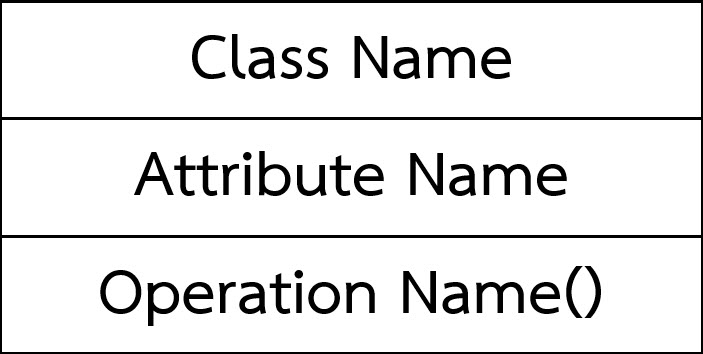
\includegraphics[width=0.3\textwidth]{Figures/table/class/11}}
			& \setstretch{1.5} {คลาส สัญลักษณ์แทนด้วยสี่เหลี่ยมแบ่งเป็น 3 ส่วน 
				ส่วนบน เป็นชื่อของ class ส่วนกลาง เป็นชื่อ Attribute และส่วนล่างเป็น Operation Name หรือ Method ใช้สำหรับเขียนฟังก์ชันในการทำงานของคลาสนั้น ๆ
				ชนิดของ Visibility ของ Method และ Attribute
				แบ่งเป็น 3 ชนิด ได้แก่
				\begin{enumerate}
					\item Public แทนสัญลักษณ์ด้วยเครื่องหมายบวก (+)
					\item Private แทนสัญลักษณ์ด้วยเครื่องหมายลบ (-)
					\item Protected แทนสัญลักษณ์ด้วยเครื่องหมายชาร์ป (#)
				\end{enumerate}
			} \\ \hline
			\raisebox{-\totalheight}{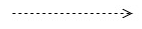
\includegraphics[width=0.3\textwidth]{Figures/table/class/1}}
			& \setstretch{1.5} {Dependency Relationship หมายความว่า คลาสที่อยู่ฝั่งต้นลูกศรสามารถเรียกใช้คลาสที่อยู่ฝั่งหัวลูกศร}
			\\ \hline
			\raisebox{-\totalheight}{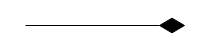
\includegraphics[width=0.35\textwidth]{Figures/3/Class/aggre}}
			& \setstretch{1.5} {Composition Relationship เป็นความสัมพันธ์ระหว่างออบเจ็กต์หรือคลาสแบบขึ้นต่อกันและมีความเกี่ยวข้องกันเสมอ} \\ \hline
			\raisebox{-\totalheight}{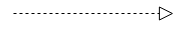
\includegraphics[width=0.3\textwidth]{Figures/3/Class/implement}}
			& \setstretch{1.5} {Realization Relationship เป็นความสัมพันธ์ระหว่าง Object หรือ Class ในลักษณะของการสืบทอดคุณสมบัติจาก Class หนึ่ง (Super class) ไปยังอีก Class หนึ่ง (Subclass)} \\ \hline
			\raisebox{-\totalheight}{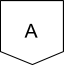
\includegraphics[width=50,height=50]{Figures/table/class/connector}}
			& \setstretch{1.5} {Connector เป็นสัญลักษณ์แทนด้วยรูปห้าเหลี่ยมและมีชื่ออยู่ตรงกลาง จะสร้างสัญลักษณ์นี้ไว้เมื่อต้องการเชื่อมต่อคลาสที่อยู่คนละหน้า} \\ \hline
		\end{tabular}
	\end{table}
	\end{center}

\newpage
  %IMAGE of class
	Class Diagram แสดงความสัมพันธ์ในรูปแบบต่างๆ ระหว่างคลาสขอระบบสแกนใบหน้าสำหรับเเคชเชียร์ อธิบายได้ตามภาพที่ \ref{Fig:MainActivity20C} ดังต่อไปนี้
	\begin{figure}[H]
		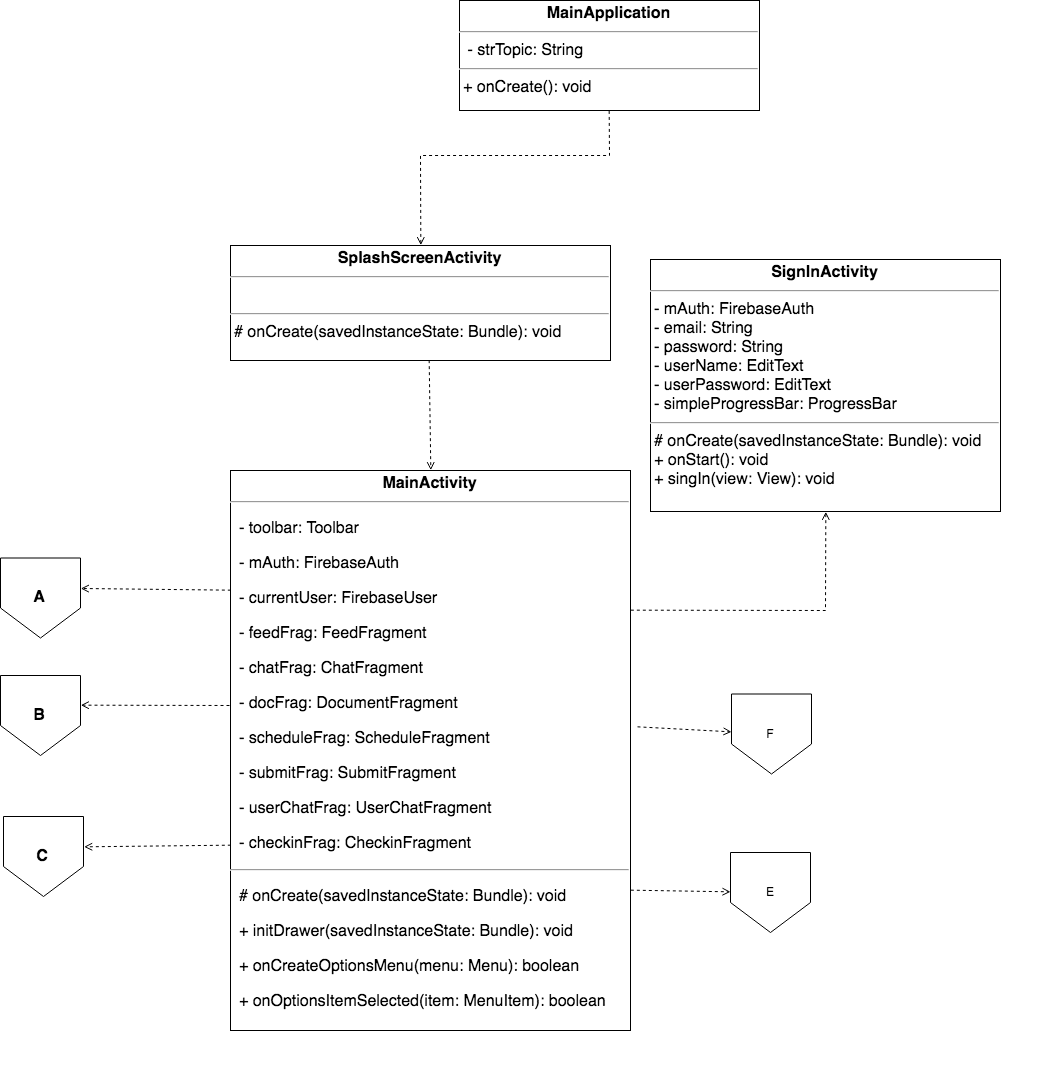
\includegraphics[width=1.0\columnwidth]{Figures/3/Class/MainActivity}
		\caption{Class Diagram ของแอปพลิเคชันระบบสแกนใบหน้าสำหรับเเคชเชียร์}
		\label{Fig:MainActivity20C}
	\end{figure}
	\begin{figure}[H]
		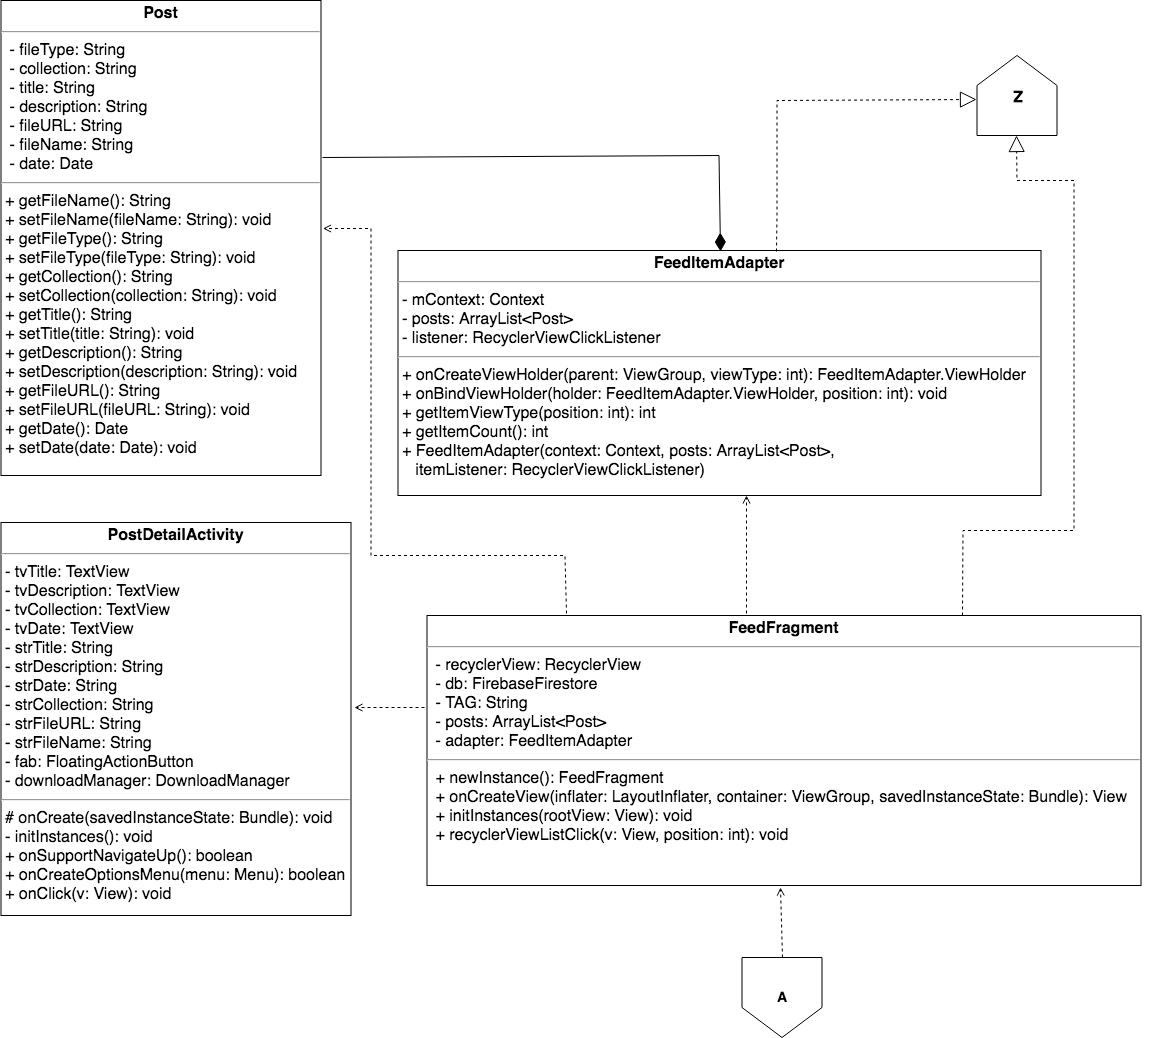
\includegraphics[width=1.0\columnwidth]{Figures/3/Class/Feed}
		\caption{Class Diagram ของแอปพลิเคชันระบบ XX}
		\label{Fig:FeedC}
	\end{figure}
\begin{sidewaysfigure}
	\begin{figure}[H]
		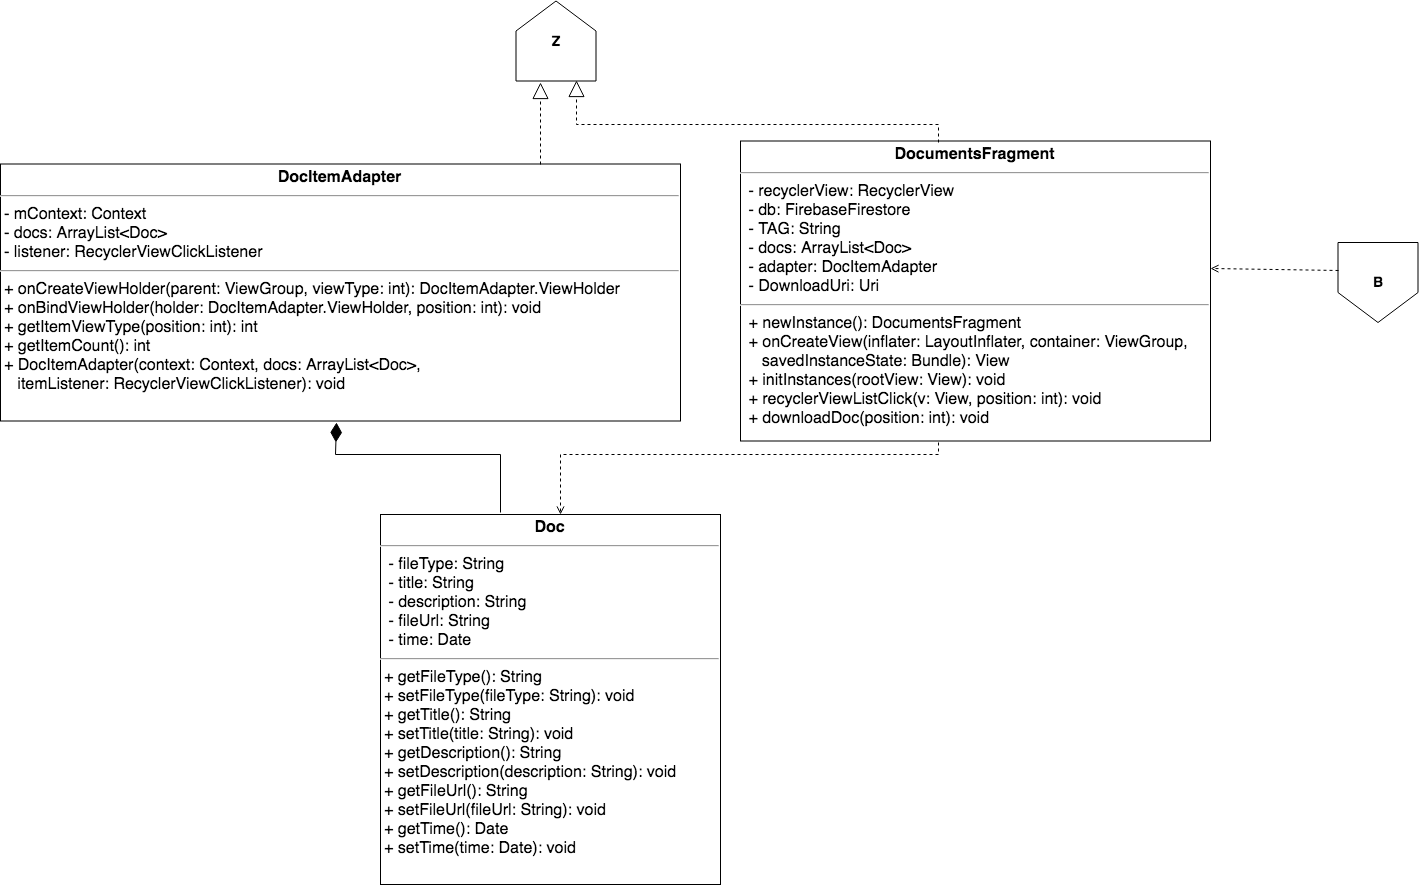
\includegraphics[width=1.0\columnwidth]{Figures/3/Class/Doc}
		\caption{Class Diagram ของแอปพลิเคชันระบบ XX}
		\label{Fig:DocC}
	\end{figure}
\end{sidewaysfigure}
	\begin{figure}[H]
		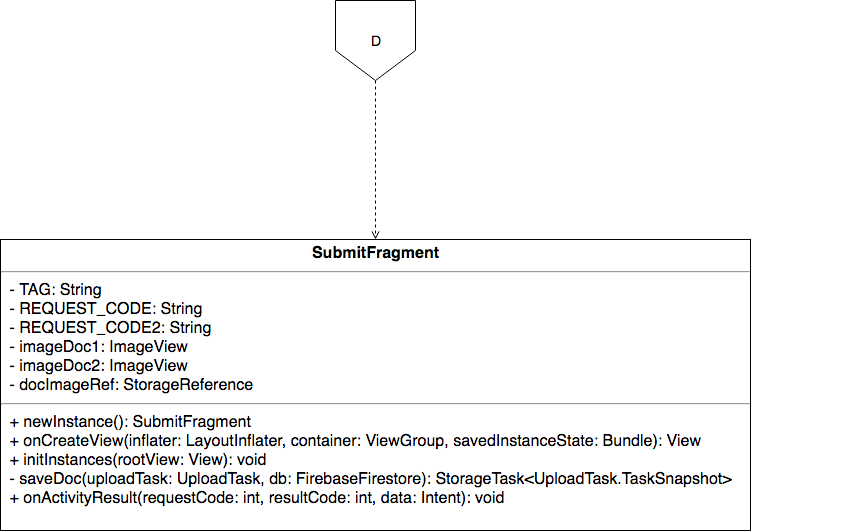
\includegraphics[width=\columnwidth]{Figures/3/Class/Submit}
		\caption{Class Diagram ของแอปพลิเคชันระบบ XX}
		\label{Fig:SubmitC}
	\end{figure}
	\begin{figure}[H]
		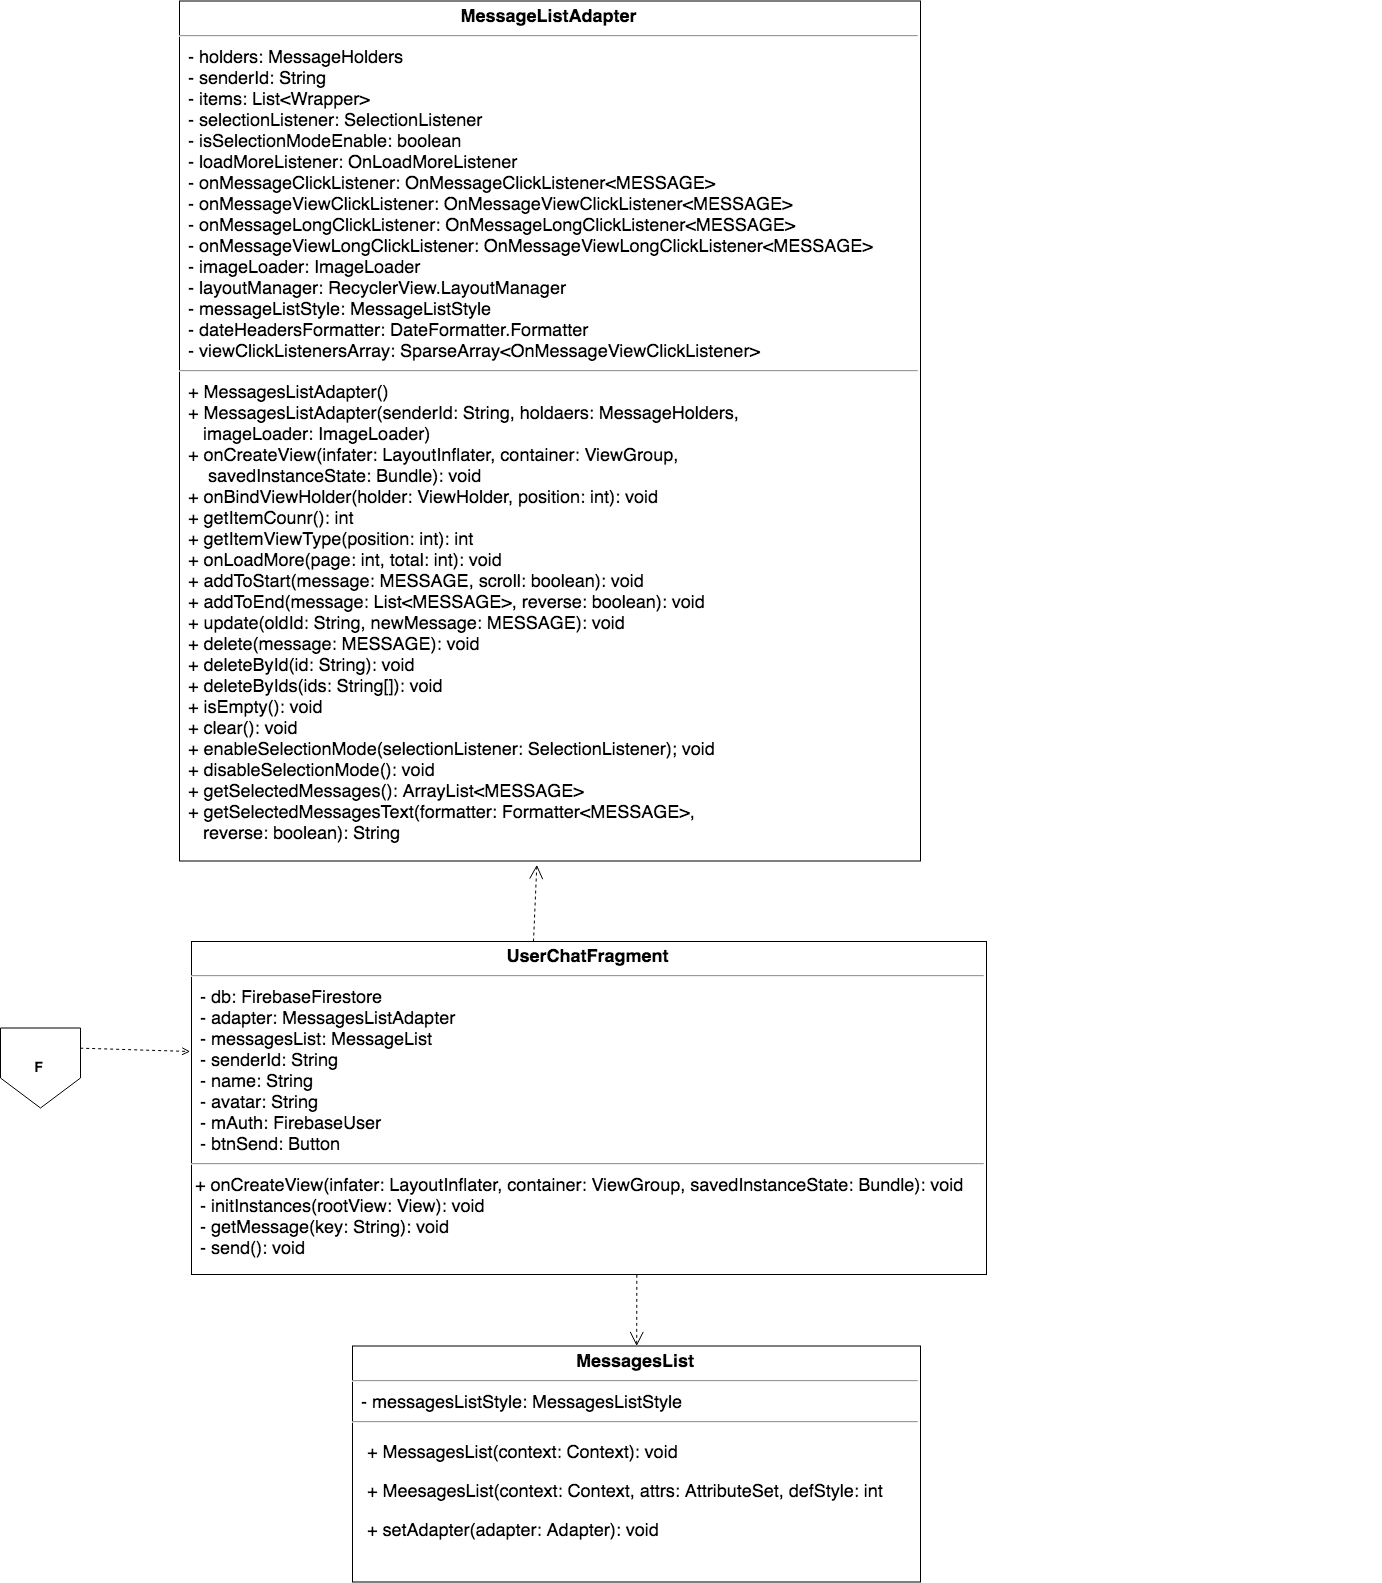
\includegraphics[width=1.0\columnwidth]{Figures/3/Class/UserChat}
		\caption{Class Diagram ของแอปพลิเคชันระบบ XX}
		\label{Fig:UserChatC}
	\end{figure}

	% TABLE of class
\newpage	
	จากรูปภาพที่ \ref{Fig:MainActivity20C} สามารถอธิบายแผนภาพ Class Diagram ได้ดังนี้
	\begin{table}[H]
		\centering
		\caption{อธิบาย Class Diagram ของคลาสพื้นฐานของระบบ}
		\label{tab:class}
		\begin{tabular}{|c|p{10cm}|}
			\hline
			\textbf{Class Diagram} & \multicolumn{1}{c|}{\textbf{คำอธิบาย}} \\ \hline
			\raisebox{-\totalheight}{MainApplication}
			& \setstretch{1.5} {คลาส MainApplication จะถูกเรียกใช้งานทุกครั้งเมื่อผู้ใช้เปิดแอปพลิเคชัน โดยวัตถุประสงค์การทำงานของคลาสนี้คือ เพื่อใช้จัดการทรัพยากรที่จำเป็นสำหรับการใช้งานในคลาสอื่น ๆ } \\ \hline
			\raisebox{-\totalheight}{SplashScreenActivity}
			& \setstretch{1.5} {คลาส SplashScreenActivity จะถูกเรียกใช้งานทุกครั้งเมื่อผู้ใช้เปิดแอปพลิเคชัน โดยวัตถุประสงค์การทำงานของคลาสคือ เพื่อใช้ตรวจสอบสถานะการเข้าสู่ระบบของผู้ใช้} \\ \hline
			\raisebox{-\totalheight}{MainActivity}
			& \setstretch{1.5} {คลาส MainActivity เป็นคลาสหลักที่ใช้ในการทำงานของแอปพลิเคชันโดยการทำงานของคลาสนี้เน้นไปที่การสร้าง Fragment เพื่อใช้แสดงข้อมูลต่าง ๆ โดยองค์ประกอบการทำงานของคลาสนี้ประกอบบไปด้วยสองส่วนหลักๆ ได้แก่ เมนูนำทาง Drawer และ Fragment Container} \\ \hline
			\raisebox{-\totalheight}{SignInActivity}
			& \setstretch{1.5} {คลาส SignInActivity เป็นคลาสที่ใช้เพื่อให้สมาชิกที่ได้ลงทะเบียนกับระบบเข้าสู่ระบบเพื่อใช้งานบริการต่าง ๆ จากระบบ} \\ \hline
	\end{tabular}
\end{table}

\newpage
จากรูปภาพที่ \ref{Fig:FeedC} สามารถอธิบายแผนภาพ Class Diagram ได้ดังนี้
\begin{table}[H]
	\centering
	\caption{อธิบาย Class Diagram ของส่วนของการแสดงข่าวสาร}
	\label{tab:class}
	\begin{tabular}{|c|p{10cm}|}
		\hline
		\textbf{Class Diagram} & \multicolumn{1}{c|}{\textbf{คำอธิบาย}} \\ \hline
		\raisebox{-\totalheight}{FeedFragment}
		& \setstretch{1.5} {คลาส FeedFragment เป็นคลาสหลักที่ใช้ในการแสดงข้อมูลข่าวสาร มีการทำงานหลักคือสืบค้นฐานข้อมูลจากไฟร์เบสเพื่อนำมาแสดง} \\ \hline
		\raisebox{-\totalheight}{FeedItemAdapter}
		& \setstretch{1.5} {คลาส FeedItemAdapter เป็นคลาสที่มีหน้าที่ในการแปลงชุดข้อมูลที่ได้จากคลาส FeedFragment แล้วคืนค่ากลับเป็นลิสต์รายการของชุดข้อมูลนั้น ๆ} \\ \hline
		\raisebox{-\totalheight}{Post}
		& \setstretch{1.5} {คลาส Post เป็นคลาสโมเดลที่กำหนดค่าต่างๆที่จำเป็นสำหรับใช้ในการสร้างลิสต์รายการของคลาส FeedItemAdapter} \\ \hline
		\raisebox{-\totalheight}{PostDetailActivity}
		& \setstretch{1.5} {คลาส PostDetailActivity เป็นคลาสที่มีหน้าที่ในการแสดงข้อมูลรายละเอียดของข่าวสารแต่ละแถวที่ได้รับจากหน้า FeedFragment ที่จะส่งข้อมูลเมื่อผู้ใช้กดที่แถวรายการข่าวสาร} \\ \hline
		\raisebox{-\totalheight}{RecyclerViewClickListener}
		& \setstretch{1.5} {คลาส RecyclerViewClickListener เป็นคลาสอินเทอร์เฟส(Interface)ที่ใช้ในการสร้างแม่แบบเมื่อคลาสใด ๆ ต้องการใช้งานสำหรับการรับค่าเมื่อผู้ใช้กดแถวในลิสต์รายการ คลาสลูกที่ทำการสืบทอดคุณสมบัติจะสามารถรับข้อมูลตำแหน่งแถวที่ผู้ใช้กดบนลิสต์รายการได้} \\ \hline
	\end{tabular}
\end{table}

\newpage
จากรูปภาพที่ \ref{Fig:DocC} สามารถอธิบายแผนภาพ Class Diagram ได้ดังนี้
\begin{table}[H]
	\centering
	\caption{อธิบาย Class Diagram ของส่วนของการแสดงรายการเอกสารในระบบ}
	\label{tab:class}
	\begin{tabular}{|c|p{10cm}|}
		\hline
		\textbf{Class Diagram} & \multicolumn{1}{c|}{\textbf{คำอธิบาย}} \\ \hline
		\raisebox{-\totalheight}{DocumentsFragment}
		& \setstretch{1.5} {คลาส DocumentsFragment เป็นคลาสที่ใช้ในการแสดงข้อมูลเอกสารที่ถูกอัพโหลดเข้าสู่ระบบโดยเจ้าหน้าที่ซึ่งจะถูกแสดงเป็นลิสต์รายการ} \\ \hline
		\raisebox{-\totalheight}{DocItemAdapter}
		& \setstretch{1.5} {คลาส DocItemAdapter เป็นคลาสที่มีหน้าที่ในการแปลงชุดข้อมูลที่ได้รับจากคลาส DocumentsFragment เป็นลิสต์รายการแล้วคืนกลับไปยังคลาส DocumentsFragment} \\ \hline
		\raisebox{-\totalheight}{Doc}
		& \setstretch{1.5} {คลาส Doc เป็นคลาสโมเดลที่กำหนดค่าต่าง ๆ ที่จำเป็นสำหรับใช้ในการสร้างลิสต์รายการของคลาส DocItemAdapter} \\ \hline
		\raisebox{-\totalheight}{RecyclerViewClickListener}
		& \setstretch{1.5} {คลาส RecyclerViewClickListener เป็นคลาสอินเทอร์เฟสที่ใช้ในการสร้างแม่แบบเมื่อคลาสใด ๆ ต้องการใช้งานสำหรับการรับค่าเมื่อผู้ใช้กดแถวในลิสต์รายการ คลาสลูกที่ทำการสืบทอดคุณสมบัติจะสามารถรับข้อมูลตำแหน่งแถวที่ผู้ใช้กดบนลิสต์รายการได้} \\ \hline
	\end{tabular}
\end{table}

\newpage
จากรูปภาพที่ \ref{Fig:SubmitC} สามารถอธิบายแผนภาพ Class Diagram ได้ดังนี้
\begin{table}[H]
	\centering
	\caption{อธิบาย Class Diagram ของส่วนของการส่งสำเนาเอกสาร}
	\label{tab:class}
	\begin{tabular}{|c|p{10cm}|}
		\hline
		\textbf{Class Diagram} & \multicolumn{1}{c|}{\textbf{คำอธิบาย}} \\ \hline
		\raisebox{-\totalheight}{SubmitFragment}
		& \setstretch{1.5} {คลาส SubmitFragment เป็นคลาสที่ใช้ในการแสดงหน้าจอส่งสำเนาเอกสาร โดยมีการดำเนินการภายในคลาสหลัก ๆ ได้แก่ การถ่ายภาพ แปลงภาพและบันทึกภาพเข้าสู่ระบบ} \\ \hline
	\end{tabular}
\end{table}

จากรูปภาพที่ \ref{Fig:UserChatC} สามารถอธิบายแผนภาพ Class Diagram ได้ดังนี้
\begin{table}[H]
	\centering
	\caption{อธิบาย Class Diagram ของส่วนของการสนทนา}
	\label{tab:class}
	\begin{tabular}{|c|p{10cm}|}
		\hline
		\textbf{Class Diagram} & \multicolumn{1}{c|}{\textbf{คำอธิบาย}} \\ \hline
		\raisebox{-\totalheight}{UserChatFragment}
		& \setstretch{1.5} {คลาส UserChatFragment เป็นคลาสที่ใช้ในการแสดงหน้าจอสนทนาสำหรับนักศึกษา เพื่อติดต่อสอบถามข้อมูลกับเจ้าหน้าที่ มีการสืบค้นข้อมูลประวัติการสนทนาเพื่อส่งไปแปลงเป็นข้อมูลลิสต์รายการที่คลาส MessagesListAdapter} \\ \hline
		\raisebox{-\totalheight}{MessagesListAdapter}
		& \setstretch{1.5} {คลาส MessagesListAdapter เป็นคลาสที่ใช้ในการแปลงชุดข้อมูลที่ได้รับจากคลาส UserChatFragment เป็นลิสต์รายการแล้วทำการคืนค่าลิสต์รายการที่ได้กลับไปยังคลาส UserChatFragment} \\ \hline 
		\raisebox{-\totalheight}{MessagesList}
		& \setstretch{1.5} {คลาส MessagesList เป็นคลาสที่ใช้ในการจัดเก็บข้อมูลภายในคลาส UserChatFragment หลังจากที่ได้ทำการสืบค้นข้อมูลการสนทนาจากไฟร์เบสเพื่อส่งไปยังคลาส MessagesListAdapter} \\ \hline
		\raisebox{-\totalheight}{RecyclerViewClickListener}
		& \setstretch{1.5} {คลาส RecyclerViewClickListener เป็นคลาสอินเทอร์เฟสที่ใช้ในการสร้างแม่แบบเมื่อคลาสใด ๆ ต้องการใช้งานสำหรับการรับค่าเมื่อผู้ใช้กดแถวในลิสต์รายการ คลาสลูกที่ทำการสืบทอดคุณสมบัติจะสามารถรับข้อมูลตำแหน่งแถวที่ผู้ใช้กดบนลิสต์รายการได้} \\ \hline
	\end{tabular}
\end{table}

\newpage
\section{Sequence Diagram}
	Sequence Diagram เป็น Diagram ที่แสดงขั้นตอนการทำงานของแต่ละ Use Case ระหว่าง Object ต่างๆ ที่ส่งข้อความถึงกันและกัน โดย Sequence Diagram จะช่วยให้มองเห็นการทำงานของภาพรวมของระบบ ส่วนประกอบสัญลักษณ์ที่ใช้ในการเขียน Sequence Diagram 
	แสดงดังตารางที่ \ref{tab:Sequences}
	
	\begin{table}[H]
		\centering
		\caption{สัญลักษณ์ของ Sequence Diagram}
		\label{tab:Sequences}
		\begin{tabular}{| c	| p{10cm} |}
		\hline
		\textbf{สัญลักษณ์} & \multicolumn{1}{c|}{\textbf{การใช้งาน}} \\ \hline
		\raisebox{-\totalheight}{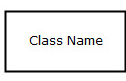
\includegraphics[width=0.17\textwidth]{Figures/table/Sequence/Sequence1}}
		& \setstretch{1.5} {Class แสดงถึงการทำงานของ Use Case ในการส่งหรือรับข้อความ แทนด้วยสัญลักษณ์สี่เหลี่ยมมีชื่อคลาสอยู่ภายใน} \\ \hline
		\raisebox{-\totalheight}{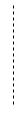
\includegraphics[height=0.08\textheight]{Figures/table/Sequence/Sequence2}}
		& \setstretch{1.5} {Lifeline หรือเส้นอายุขัย แสดงช่วงเวลาตั้งแต่เริ่มสร้าง object ในคลาสนั้น จนกระทั่ง object นั้นถูกทำลาย สัญลักษณ์แทนด้วยเส้นประ} \\ \hline
		\raisebox{-\totalheight}{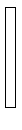
\includegraphics[height=0.08\textheight]{Figures/table/Sequence/Sequence3}}
		& \setstretch{1.5} {Focus of control หรือจุดควบคุม เป็นจุดควบคุมที่ object ใช้ทำการส่งหรือรับข้อความ สัญลักษณ์แทนด้วยสี่เหลี่ยม} \\ \hline
		\raisebox{-\totalheight}{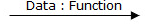
\includegraphics[width=0.3\textwidth]{Figures/table/Sequence/Sequence4}}
		& \setstretch{1.5} {Message คือ ข้อความที่รับส่งระหว่าง Object สัญลักษณ์แทนด้วยลูกศรและประกอบด้วย 2 ส่วน คือ ข้อมูล (Data) และฟังก์ชัน (Function)} \\ \hline
		\raisebox{-\totalheight}{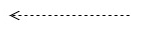
\includegraphics[width=0.3\textwidth]{Figures/table/Sequence/Sequence5}}
		& \setstretch{1.5} {Return Message เป็นข้อมูลที่ส่งกลับหลังจากทำงานเสร็จ} \\ \hline
		\raisebox{-\totalheight}{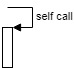
\includegraphics[height=0.08\textheight]{Figures/3/selfcall}}
		& \setstretch{1.5} {Self call เป็นการเรียกฟังชันก์การทำงานภายในตัวเอง} \\ \hline
		\raisebox{-\totalheight}{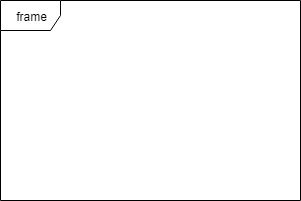
\includegraphics[height=0.1\textheight,width=0.3\textwidth]{Figures/3/frame}}
		& \setstretch{1.5} {สร้างกรอบการทำงานของโปรแกรม เพื่อให้รู้ขอบเขตของการทำงานเช่น ลูป(loop)} \\ \hline
		\end{tabular}
	\end{table}
%
%	Sequence Diagram ที่ใช้อธิบายการทำงานของระบบกองทุนเงินให้กู้ยืมเพื่อการศึกษา คณะวิทยสศาสตร์ มหาวิทยาลัยอุบลราชธานี มีรายละเอียดดังต่อไปนี้

\newpage
	\begin{landscape}
	\begin{figure}[H]
		\centering
		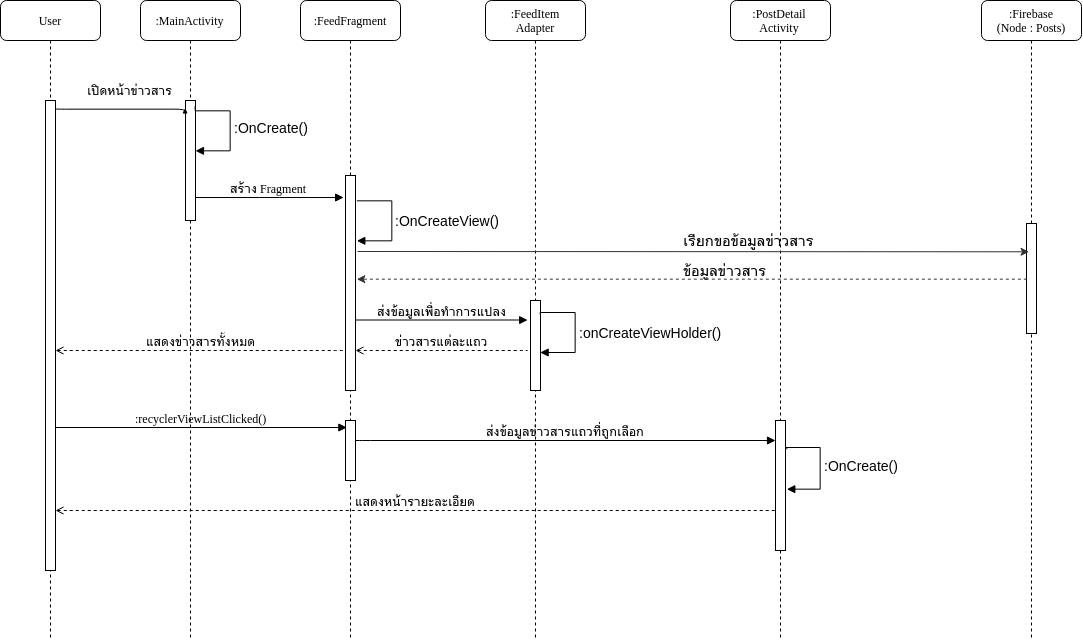
\includegraphics[width=0.95\columnwidth]
		{Figures/3/Sequence/feed}
		\caption{Sequence Diagram การแสดงข่าวสาร}
		\label{Fig:Sequence-feed}
	\end{figure}
  \end{landscape}

	จากภาพที่ \ref{Fig:Sequence-feed} สามารถอธิบายแผนภาพ Sequence Diagram แสดงข่าวสาร ได้ดังนี้ เมื่อ
	ผู้ใช้เปิดโปรแกรมระบบจะเรียกใช้เมธอด onCreate() ที่คลาส MainActivity ระบบจะทำการสร้าง
	Fragment ขึ้นมาโดยใช้เมธอด onCreate() ที่คลาส FeedFragment เมื่อ FeedFragment ถูกติดตั้งบน MainActivity เมธอด callData() จะสืบค้นข้อมูลจากฐานข้อมูลบน Firebase FireStore และส่งข้อมูลที่ได้ไปแปลงที่คลาส FeedItemAdapter โดยมีการคืนค่าเป็นข้อมูลข่าวสารแต่ละแถวและในขั้นตอนสุดท้ายคลาส FeedFragment จะทำการแสดงรายการข้อมูลข่าวสารทั้งหมดออกทางหน้าจอ หากผู้ใช้มีการกดเลือกข่าวสารบางแถวคลาส FeedFragment จะทำการเรียกใช้ PostDetailActivity เพื่อแสดงรายละเอียดข้อมูลข่าวสารของแถวที่ถูกเลือก
	\begin{sidewaysfigure}
	\begin{figure}[H]
		\centering
		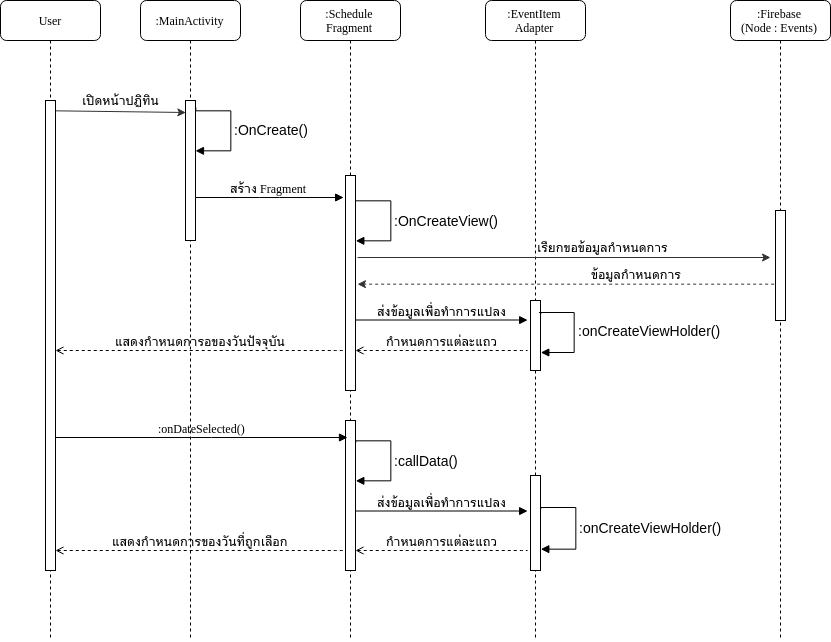
\includegraphics[width=0.8\columnwidth]
		{Figures/3/Sequence/calendar}
		\caption{Sequence Diagram การแสดงปฏิทินกำหนดการ}
		\label{Fig:Sequence-calendar}
	\end{figure}
	\end{sidewaysfigure}
	\newpage
	จากภาพที่ \ref{Fig:Sequence-calendar} สามารถอธิบายแผนภาพ Sequence Diagram แสดงปฏิทินกำหนดการ ได้ดังนี้ เมื่อ
	ผู้ใช้เปิดโปรแกรมระบบจะเรียกใช้เมธอด onCreate() ที่คลาส MainActivity ระบบจะทำการสร้าง
	Fragment ขึ้นมาโดยใช้เมธอด onCreate() ที่คลาส ScheduleFragment เมื่อ ScheduleFragment ถูกติดตั้งบน MainActivity เมธอด callData() จะสืบค้นข้อมูลกำหนดการของวันปัจจุบันจากฐานข้อมูลบน Firebase FireStore และส่งข้อมูลที่ได้ไปแปลงที่คลาส Schedule-ItemAdapter โดยมีการคืนค่าเป็นข้อมูลกำหนดการแต่ละแถวและในขั้นตอนสุดท้ายคลาส Schedule-Fragment จะทำการแสดงรายการกำหนดการวันปัจจุบันออกทางหน้าจอ หากผู้ใช้มีการกดเลือกวันที่ที่ต้องการทราบกำหนดการจากปฏิทินคลาส ScheduleFragment จะทำการเรียกใช้ callData() อีกครั้งโดยสืบค้นข้อมูลกำหนดการของวันที่ถูกเลือกจากฐานข้อมูลบน Firebase FireStore และส่งข้อมูลที่ได้ไปแปลงที่คลาส ScheduleItemAdapter โดยมีการคืนค่าเป็นข้อมูลแต่กำหนดการละแถวและในขั้นตอนสุดท้ายคลาส ScheduleFragment จะทำการแสดงรายการกำหนดการวันที่ผู้ใช้เลือกออกทางหน้าจอ

	\begin{sidewaysfigure}
	\begin{figure}[H]
		\centering
		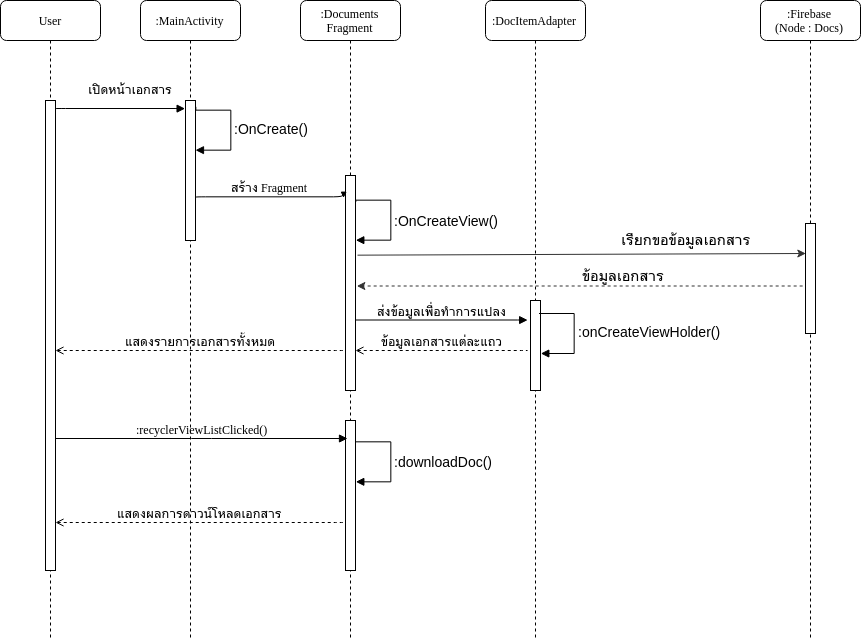
\includegraphics[width=0.8\columnwidth]
		{Figures/3/Sequence/doc}
		\caption{Sequence Diagram การแสดงดาวน์โหลดเอกสาร}
		\label{Fig:Sequence-doc}
	\end{figure}
	\end{sidewaysfigure}
	\newpage
	จากภาพที่ \ref{Fig:Sequence-doc} สามารถอธิบายแผนภาพ Sequence Diagram แสดงดาวน์โหลดเอกสาร ได้ดังนี้ เมื่อผู้ใช้เปิดโปรแกรมระบบจะเรียกใช้เมธอด onCreate() ที่คลาส MainActivity ระบบจะทำการสร้าง
	Fragment ขึ้นมาโดยใช้เมธอด onCreate() ที่คลาส DocumentsFragment เมื่อ DocumentsFragment ถูกติดตั้งบน MainActivity เมธอด initInstances() จะสืบค้นข้อมูลเอกสารทั้งหมดจากฐานข้อมูลบน Firebase FireStore และส่งข้อมูลที่ได้ไปแปลงที่คลาส DocItem-Adapter โดยมีการคืนค่าเป็นข้อมูลเอกสารแต่ละแถวและในขั้นตอนสุดท้ายคลาส Documents-Fragment จะทำการแสดงรายการกำหนดการวันปัจจุบันออกทางหน้าจอ

	\begin{sidewaysfigure}
	\begin{figure}[H]
		\centering
		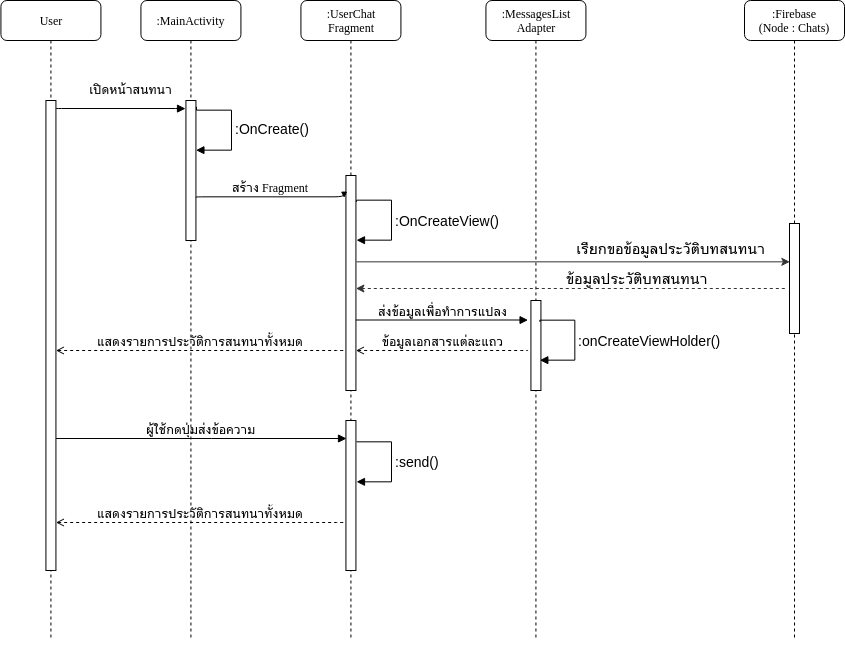
\includegraphics[width=0.8\columnwidth]
		{Figures/3/Sequence/chat}
		\caption{Sequence Diagram การแสดงบทสนทนา}
		\label{Fig:Sequence-chat}
	\end{figure}
	\end{sidewaysfigure}
	\newpage
	จากภาพที่ \ref{Fig:Sequence-chat} สามารถอธิบายแผนภาพ Sequence Diagram แสดงการสนทานา ได้ดังนี้ เมื่อผู้ใช้เปิดโปรแกรมระบบจะเรียกใช้เมธอด onCreate() ที่คลาส MainActivity ระบบจะทำการสร้าง
	Fragment ขึ้นมาโดยใช้เมธอด onCreate() ที่คลาส UserChatFragment เมื่อ UserChatFrag-ment ถูกติดตั้งบน MainActivity เมธอด getMessage() จะสืบค้นข้อมูลประวัติการสนทนาของผู้ใช้คนปัจจุบันทั้งหมดจากฐานข้อมูลบน Firebase FireStore และส่งข้อมูลที่ได้ไปแปลงที่คลาส MessagesListAdapter โดยมีการคืนค่าเป็นข้อมูลรายการประวัติการสนทนาทั้งหมดและในขั้นตอนสุดท้ายคลาส User-ChatFragment จะทำการแสดงรายการประวัติการสนทนาทั้งหมดออกทางหน้าจอ เมื่อผู้ใช้พิมพ์ข้อความและกดปุ่มส่งระบบจะเรียกให้เมธอด send() เพื่อทำการบันทึกข้อมูลไว้บน Firebase FireStore และทำการแสดงข้อมูลรายการประวัติการสนทนาทั้งหมดที่ถูกอัพเดท

	\begin{sidewaysfigure}
	\begin{figure}[H]
		\centering
		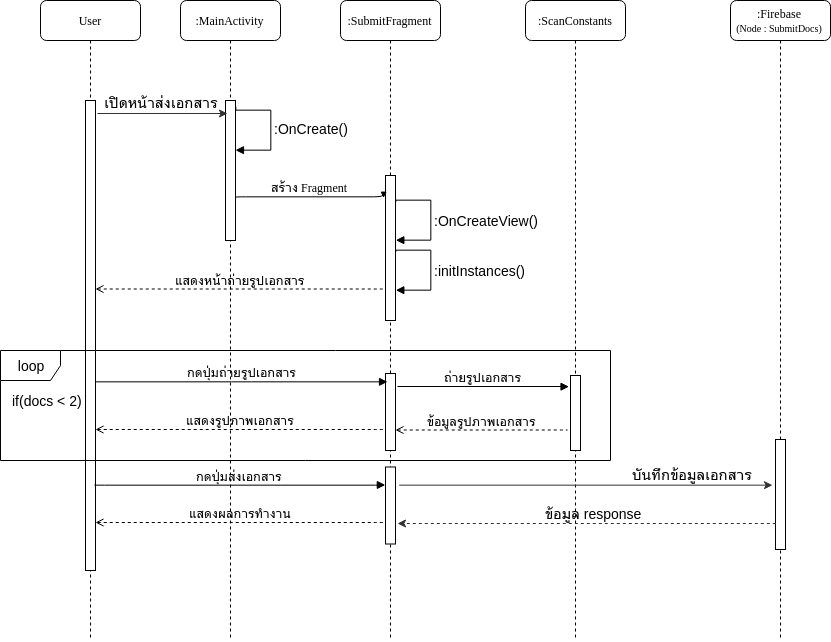
\includegraphics[width=0.8\columnwidth]
		{Figures/3/Sequence/submit}
		\caption{Sequence Diagram แสดงส่งเอกสารตรวจสอบ}
		\label{Fig:Sequence-submit}
	\end{figure}
	\end{sidewaysfigure}
	\newpage
	จากภาพที่ \ref{Fig:Sequence-submit} สามารถอธิบายแผนภาพ Sequence Diagram แสดงส่งเอกสารตรวจสอบ ได้ดังนี้ เมื่อผู้ใช้เปิดโปรแกรมระบบจะเรียกใช้เมธอด onCreate() ที่คลาส MainActivity ระบบจะทำการสร้าง
	Fragment ขึ้นมาโดยใช้เมธอด onCreate() ที่คลาส SubmitFragment เมื่อ Submit-Fragment ถูกติดตั้งบน MainActivity เมธอด initInstances() จะถูกเรียกเพื่อสร้างหน้าจอแสงดผลเมื่อผู้ใช้กดปุ่มถ่ายรูประบบจะเรียกใช้ไลบรารี่ ScanConstants เพื่อถ่ายภาพเอกสารและรอให้ผู้ใช้ถ่ายครบทั้งสองแผ่นจึงจะแสดงปุ่มกดส่งเอกสารเพื่อตรวจสอบ
\newpage	 
	
\section{โครงสร้างฐานข้อมูลไฟร์เบส(Firebase Database Stucture)}
Firebase Database นั้นเป็น Database แบบ NoSQL และเป็น JSON database ที่มีโครงสร้างที่เป็น Key และ Value จัดเก็บข้อมูลในลักษณะโหนด หากต้องการเรียกงานจะเรียกใช้โดย
การท่องไปยังโหนดที่ต้องการ ส่วนประกอบสัญลักษณ์ที่ใช้ในการเขียนโครงสร้างฐานข้อมูลแบบ Firebase
แสดงดังตารางที่ \ref{tab:DB}

\begin{table}[H]
	\centering
	\caption{สัญลักษณ์ของโครงสร้างฐานข้อมูลแบบ Firebase}
	\label{tab:DB}
	\begin{tabular}{| c	| p{10cm} |}
		\hline
		\textbf{สัญลักษณ์} & \multicolumn{1}{c|}{\textbf{คำอธิบาย}} \\ \hline
		\raisebox{-\totalheight}{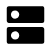
\includegraphics[width=0.1\textwidth]{Figures/3/DB/dbroot}}
		& \setstretch{1.5} {Database เป็นการเรียกชื่อแทนโหนด(Node)บนสุดที่ใช้ในการเก็บข้อมูล} \\ \hline
		\raisebox{-\totalheight}{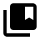
\includegraphics[width=0.1\textwidth]{Figures/3/DB/dbcollection}}
		& \setstretch{1.5} {Collection เป็นการเรียกชื่อแทนของการเก็บหลาย ๆ เอกสารไว้ด้วยกัน} \\ \hline
		\raisebox{-\totalheight}{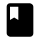
\includegraphics[width=0.1\textwidth]{Figures/3/DB/dbdoc}}
		& \setstretch{1.5} {Document เป็นการเรียกชื่อแทนหน่วยการเก็บของข้อมูลใน Cloud Firestore ภายในจะประกอบไปด้วย ชื่อของ Document  ชื่อของคีย์ (key) และ ค่าข้อมูล (value) โดยชื่อของ Document ห้ามซ้ำกัน ซึ่งใน Cloud Firestore สามารถระบุประเภทของข้อมูลได้ 9 ประเภทได้แก่ boolean, number, string, geo point, timestamp, array, object, reference และ null} \\ \hline
	\end{tabular}
\end{table}
	\begin{figure}[H]
	\centering
	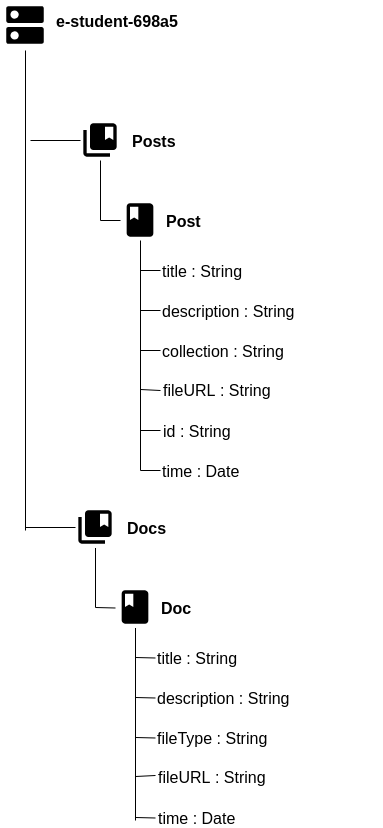
\includegraphics[width=0.7\columnwidth]
	{Figures/3/DB/DB1}
	\caption{โครงสร้างฐานข้อมูลแบบ Firebase}
	\label{Fig:DB1}
	\end{figure}

	\begin{figure}[H]
	\centering
	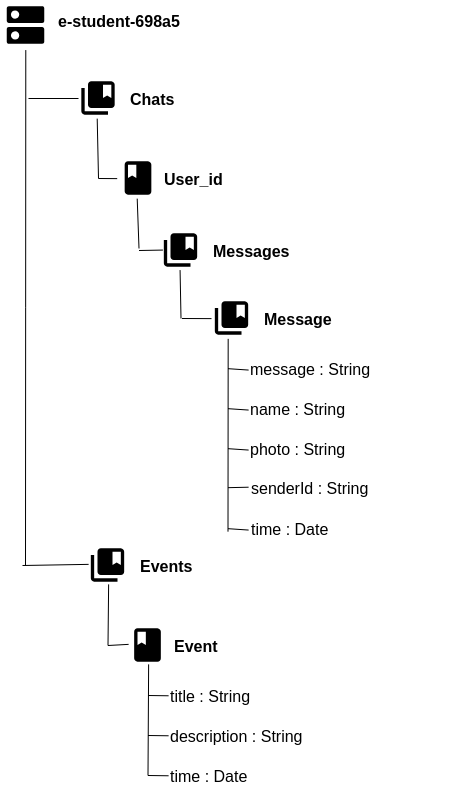
\includegraphics[width=0.9\columnwidth]
	{Figures/3/DB/DB2}
	\caption{โครงสร้างฐานข้อมูลแบบ Firebase(ต่อ)}
	\label{Fig:DB2}
\end{figure}
	\begin{figure}[H]
	\centering
	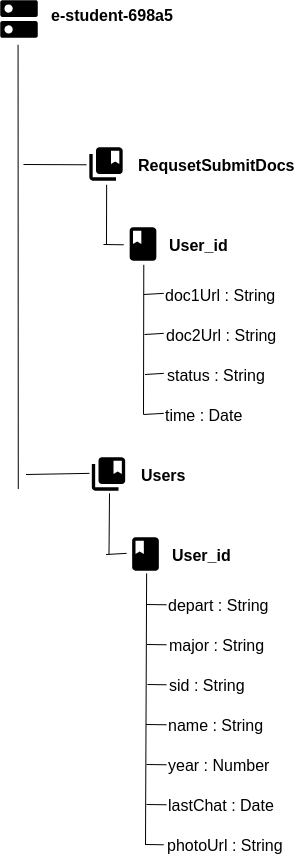
\includegraphics[width=0.55\columnwidth]
	{Figures/3/DB/DB3}
	\caption{โครงสร้างฐานข้อมูลแบบ Firebase(ต่อ)}
	\label{Fig:DB3}
\end{figure}
	\begin{figure}[H]
	\centering
	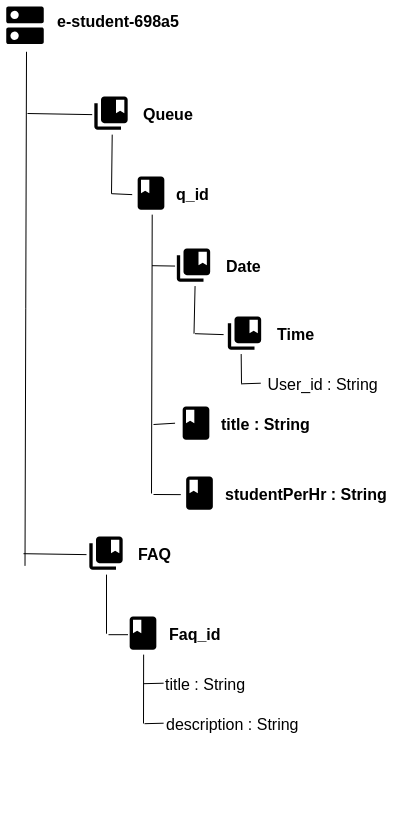
\includegraphics[width=0.7\columnwidth]
	{Figures/3/DB/DB4}
	\caption{โครงสร้างฐานข้อมูลแบบ Firebase(ต่อ)}
	\label{Fig:DB4}
\end{figure}

\newpage
จากรูที่ \ref{Fig:DB1}-\ref{Fig:DB4} สามารถอธิบายโครงสร้างของข้อมูลได้ดังนี้
\begin{figure}[H]
\centering
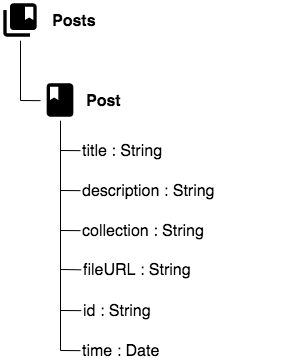
\includegraphics[width=0.5\columnwidth]
{Figures/3/DB/nodePost}
\caption{โหนดเก็บข้อมูลประกาศ}
\label{Fig:DB4}
\end{figure}
\begin{table}[H]
	\centering
	\caption{อธิบายโหนดที่ใช้เก็บข้อมูลประกาศ}
	\label{my-label1}
	\begin{tabular}{|c|p{10cm}|}
		\hline
		\multicolumn{1}{|c|}{\textbf{Key}} & \multicolumn{1}{c|}{\textbf{คำอธิบาย}} \\ \hline
		Posts & โหนดสำหรับเก็บข้อมูลประกาศทั้งหมด \\ \hline
		Post &  สำหรับเก็บข้อมูลแต่ละประกาศ \\ \hline
		title & สำหรับเก็บชื่อหัวข้อประกาศ \\ \hline
		description & สำหรับเก็บรายละเอียดประกาศ  \\ \hline
		collection & สำหรับเก็บประเภทของประกาศได้แก่ สาธารณะและเฉพาะบุคคล \\ \hline
		fileURL & สำหรับเก็บ url ของเอกสารแนบประกาศ \\ \hline
		id & สำหรับเก็บรหัสของประกาศ \\ \hline
		time & สำหรับเก็บเวลาที่ประกาศ \\ \hline
	\end{tabular}
\end{table}

\newpage
\begin{figure}[H]
	\centering
	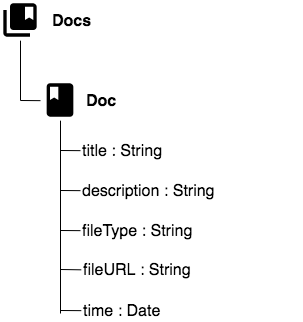
\includegraphics[width=0.5\columnwidth]
	{Figures/3/DB/nodeDoc}
	\caption{โหนดเก็บข้อมูลเอกสารที่เกี่ยวข้อง}
	\label{Fig:DB4}
\end{figure}
\begin{table}[H]
	\centering
	\caption{อธิบายโหนดที่ใช้เก็บข้อมูลเอกสารที่เกี่ยวข้อง}
	\label{my-label1}
	\begin{tabular}{|c|p{10cm}|}
		\hline
		\multicolumn{1}{|c|}{\textbf{Key}} & \multicolumn{1}{c|}{\textbf{คำอธิบาย}} \\ \hline
		Docs & โหนดสำหรับเก็บข้อมูลของเอกสารที่เกี่ยวข้องทั้งหมด \\ \hline
		Doc &  สำหรับเก็บข้อมูลเอกสารแต่ละฉบับ \\ \hline
		title & สำหรับเก็บชื่อหัวเรื่องของเอกสาร \\ \hline
		description & สำหรับเก็บรายละเอียดของเอกสาร \\ \hline
		fileType & สำหรับนามสกุลไฟล์เอกสาร เช่น .pdf .png เป็นต้น \\ \hline
		fileURL & สำหรับเก็บ url ของเอกสาร\\ \hline
		time & สำหรับเก็บเวลาที่ถูกอัพโหลดเข้าสู่ระบบโดยเจ้าหน้าที่\\ \hline
	\end{tabular}
\end{table}

\newpage
\begin{figure}[H]
	\centering
	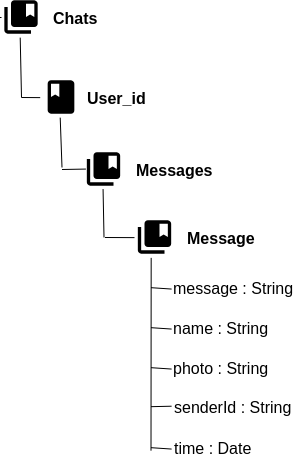
\includegraphics[width=0.4\columnwidth]
	{Figures/3/DB/nodeChat}
	\caption{โหนดเก็บข้อมูลประวัติการสนทนา}
	\label{Fig:DB4}
\end{figure}
\begin{table}[H]
	\centering
	\caption{อธิบายโหนดที่ใช้เก็บข้อมูลประวัติการสนทนา}
	\label{my-label1}
	\begin{tabular}{|c|p{10cm}|}
		\hline
		\multicolumn{1}{|c|}{\textbf{Key}} & \multicolumn{1}{c|}{\textbf{คำอธิบาย}} \\ \hline
		Chats & โหนดสำหรับเก็บข้อมูลประวัติการสนทนาทั้งหมด \\ \hline
		User\_id &  สำหรับเก็บประวัติการสนทนาของผู้ใช้แต่ละคน \\ \hline
		Messages & สำหรับเก็บประวัติการสนทนาทั้งหมดของผู้ใช้ \\ \hline
		Message & สำหรับเก็บข้อมูลของแต่ละข้อความ \\ \hline
		message & สำหรับเก็บข้อความ \\ \hline
		name & สำหรับเก็บชื่อของผู้ส่งข้อความ\\ \hline
		photo & สำหรับเก็บ url รูปภาพของผู้ส่งข้อความ\\ \hline
		senderId & สำหรับเก็บรหัสของผู้ส่งข้อความ\\ \hline
		time & สำหรับเก็บเวลาที่ข้อความถูกส่ง\\ \hline
	\end{tabular}
\end{table}

\newpage
\begin{figure}[H]
	\centering
	\includegraphics[width=0.5\columnwidth]
	{Figures/3/DB/nodeEvent}
	\caption{โหนดเก็บข้อมูลกำหนดการ}
	\label{Fig:DB4}
\end{figure}
\begin{table}[H]
	\centering
	\caption{อธิบายโหนดที่ใช้เก็บข้อมูลกำหนดการ}
	\label{my-label1}
	\begin{tabular}{|c|p{10cm}|}
		\hline
		\multicolumn{1}{|c|}{\textbf{Key}} & \multicolumn{1}{c|}{\textbf{คำอธิบาย}} \\ \hline
		Events & โหนดสำหรับเก็บข้อมูลของกำหนดการทั้งหมด \\ \hline
		Event & สำหรับเก็บข้อมูลของแต่ละกำหนดการ \\ \hline
		title & สำหรับเก็บชื่อหัวข้อของกำหนดการ \\ \hline
		description & สำหรับเก็บรายละเอียดของกำหนดการ\\ \hline
		time & สำหรับเก็บเวลาของกำหนดการ\\ \hline
	\end{tabular}
\end{table}

\newpage
\begin{figure}[H]
	\centering
	\includegraphics[width=0.4\columnwidth]
	{Figures/3/DB/nodeReq}
	\caption{โหนดเก็บข้อมูลการยื่นสำเนาเอกสารเพื่อตรวจสอบของนักศึกษา}
	\label{Fig:DB4}
\end{figure}
\begin{table}[H]
	\centering
	\caption{อธิบายโหนดที่ใช้เก็บข้อมูลการยื่นสำเนาเอกสารเพื่อตรวจสอบของนักศึกษา}
	\label{my-label1}
	\begin{tabular}{|c|p{10cm}|}
		\hline
		\multicolumn{1}{|c|}{\textbf{Key}} & \multicolumn{1}{c|}{\textbf{คำอธิบาย}} \\ \hline
		RusetSubmitDocs & โหนดสำหรับเก็บข้อมูลการยื่นสำเนาเอกสารเพื่อตรวจสอบของนักศึกษาทั้งหมด \\ \hline
		User\_id & สำหรับเก็บข้อมูลของแต่ละสำเนาเอกสารของนักศึกษาแต่ละคน \\ \hline
		doc2 & สำหรับเก็บ url ของภาพถ่ายสำเนาเอกสารฉบับที่ 1\\ \hline
		doc2 & สำหรับเก็บ url ของภาพถ่ายสำเนาเอกสารฉบับที่ 2\\ \hline
		status & สำหรับเก็บผลการตรวจสอบของเจ้าหน้าที่ \\ \hline
		time & สำหรับเก็บเวลาที่สำเนาเอกสารถูกเพิ่มเข้าสู่ระบบ \\ \hline
	\end{tabular}
\end{table}

\newpage
\begin{figure}[H]
	\centering
	\includegraphics[width=0.35\columnwidth]
	{Figures/3/DB/nodeUser}
	\caption{โหนดเก็บข้อมูลของนักศึกษา}
	\label{Fig:DB4}
\end{figure}
\begin{table}[H]
	\centering
	\caption{อธิบายโหนดที่ใช้เก็บข้อมูลของนักศึกษา}
	\label{my-label1}
	\begin{tabular}{|c|p{10cm}|}
		\hline
		\multicolumn{1}{|c|}{\textbf{Key}} & \multicolumn{1}{c|}{\textbf{คำอธิบาย}} \\ \hline
		Users & โหนดสำหรับเก็บข้อมูลของนักศึกษา \\ \hline
		User\_id & สำหรับเก็บข้อมูลของนักศึกษาแต่ละคน \\ \hline
		depart & สำหรับเก็บภาควิชาของนักศึกษา\\ \hline
		major & สำหรับเก็บสาขาของนักศึกษา\\ \hline
		sid & สำหรับเก็บรหัสประจำตัวนักศึกษา \\ \hline
		name & สำหรับเก็บชื่อของนักศึกษา \\ \hline
		year & สำหรับเก็บชั้นปีของนักศึกษา \\ \hline
		lastChat & สำหรับเก็บเวลาที่สนทนากับเจ้าหน้าที่ล่าสุด \\ \hline
		photoUrl & สำหรับเก็บ url รูปภาพโปรไฟล์ (Profile) \\ \hline
	\end{tabular}
\end{table}

\newpage
\begin{figure}[H]
	\centering
	\includegraphics[width=0.5\columnwidth]
	{Figures/3/DB/nodeQueue}
	\caption{โหนดเก็บข้อมูลการจองคิวของนักศึกษา}
	\label{Fig:DB4}
\end{figure}
\begin{table}[H]
	\centering
	\caption{อธิบายโหนดที่ใช้เก็บข้อมูลการจองคิวของนักศึกษา}
	\label{my-label1}
	\begin{tabular}{|c|p{10cm}|}
		\hline
		\multicolumn{1}{|c|}{\textbf{Key}} & \multicolumn{1}{c|}{\textbf{คำอธิบาย}} \\ \hline
		Queue & โหนดสำหรับเก็บข้อมูลการจองคิวของนักศึกษาทั้งหมด \\ \hline
		q\_id &  สำหรับเก็บข้อมูลของการจองคิวแต่ละครั้งที่เปิดจองคิว \\ \hline
		Date &  สำหรับเก็บวันที่สำหรับส่งเอกสาร\\ \hline
		Time &  สำหรับเก็บรายชื่อของนักศึกษาที่ทำการจองคิวในส่งเอกสารเวลานั้น ๆ\\ \hline
		User\_id & สำหรับเก็บรหัสของนักศึกษา \\ \hline
		title & สำหรับเก็บชื่อหัวเรื่องกำหนดการการจองคิว \\ \hline
		studentPerHr & สำหรับเก็บจำนวนนักศึกษาต่อชั่วโมง \\ \hline
	\end{tabular}
\end{table}

\newpagedr
\begin{figure}[H]
	\centering
	\includegraphics[width=0.4\columnwidth]
	{Figures/3/DB/nodeFaq}
	\caption{โหนดเก็บข้อมูลคำถามที่พบบ่อย}
	\label{Fig:DB4}
\end{figure}
\begin{table}[H]
	\centering
	\caption{อธิบายโหนดที่ใช้เก็บข้อมูลคำถามที่พบบ่อย}
	\label{my-label1}
	\begin{tabular}{|c|p{10cm}|}
		\hline
		\multicolumn{1}{|c|}{\textbf{Key}} & \multicolumn{1}{c|}{\textbf{คำอธิบาย}} \\ \hline
		Queue & โหนดสำหรับเก็บข้อมูลคำถามที่พบบ่อยทั้งหมด \\ \hline
		Faq\_id & สำหรับเก็บข้อมูลคำถามที่พบบ่อยแต่ละรายการ \\ \hline
		title & สำหรับเก็บคำถาม \\ \hline
		description & สำหรับเก็บคำตอบ \\ \hline
	\end{tabular}
\end{table}

\chapter{การพัฒนาระบบ}
หลังจากที่ได้มีการเตรียมความพร้อมสำหรับการพัฒนาในด้านต่าง ไม่ว่าจะเป็นที่มาและความสำคัญของปัญหา เทคโนโลยีที่มีความเหมาะสมกับระบบ และการออกแบบระบบการทำงานรวมไปถึงโครงสร้างของข้อมูล ในบทนี้จะเป็นการพูดถึงการสร้างระบบที่ได้มีการออกแบบไว้ในบทที่แล้วจะถูกนำเสนอในบทนี้ โดยการพัฒนาระบบแบ่งได้เป็นส่วนต่าง ๆ ดังนี้
	\begin{enumerate}[label=4.\arabic*]
		\item การพัฒนาเว็บแอปพลิเคชัน
		\item การพัฒนาเว็บแอปพลิเคชันแอนดรอยด์แอปพลิเคชัน
	\end{enumerate}	

\section{การพัฒนาเว็บแอปพลิเคชัน}
	การพัฒนาระบบกองทุนเงินให้กู้ยืมเพื่อการศึกษาสำหรับเว็บแอปพลิเคชันนั้นวัตถุประสงค์หลังเพื่อสร้างความสะดวกต่อการกำงานของเจ้าหน้าที่อันเนื่องมาจากข้อจำกัดบางประการหากใช้ระบบทำงานบนอุปกรณ์สมาร์ทโฟนเพียงอย่างเดียว โดยตัวเว็บแอปพลิเคชันนี้ถูกพัฒนาขึ้นด้วย Vue.js มีรายละเอียดการทำงานดังนี้
	
	\subsection{การเชื่อมต่อ Cloud Firestore}bsection,
	ในการเชื่อมต่อเว็บแอปพลิเคชันกับไฟร์เบสเพื่อใช้บริการต่างๆ ของไฟร์เบส ทำได้ดังนี้
	\begin{figure}[H]
		{\setstretch{1.0}\begin{lstlisting}
export default {
	apiKey: "XXXXXXXXXXXXXXXXXXXXXXXXXXXXXXXXXXXXXXX",
	authDomain: "e-student-698a5.firebaseapp.com",
	databaseURL: "https://e-student-698a5.firebaseio.com",
	projectId: "e-student-698a5",
	storageBucket: "e-student-698a5.appspot.com",
	messagingSenderId: "000000000000"
}
			\end{lstlisting}}
		\caption{ไฟล์ firebaseConfig.js}
		\label{Fig:firebaseConfig}
	\end{figure}
	จากภาพที่ \ref{Fig:firebaseConfig} โครงสร้างของไฟล์ firebaseConfig.js สามารถอธิบายการทำงานได้ดังนี้
	\begin{itemize}[label={--}]
		\item บรรทัดที่  1	     เป็นการส่งออกโมดูลเพื่อใช้งานในไฟล์อื่น
		\item บรรทัดที่  2 -7	เป็นการตั้งค่าระบุตัวตนเพื่อใช้งานบริการไฟร์เบส
	\end{itemize}
	
	\begin{figure}[H]
		{\setstretch{1.0}\begin{lstlisting}
import firebase from 'firebase'
import 'firebase/firestore'
import firebaseConfig from './firebaseConfig'

export default firebase.initializeApp(firebaseConfig)
			\end{lstlisting}}
		\caption{ไฟล์ firebaseInit.js}
		\label{Fig:firebaseConfig}
	\end{figure}
	จากภาพที่ \ref{Fig:firebaseConfig} โครงสร้างของไฟล์ firebaseInit.js สามารถอธิบายการทำงานได้ดังนี้
	\begin{itemize}[label={--}]
		\item บรรทัดที่  1	     เป็นการนำเข้าไลบรารีของไฟร์เบส
		\item บรรทัดที่  2 	    เป็นการนำเข้าบริการ Cloud Firestore ของไฟร์เบส 
		\item บรรทัดที่  8       เป็นการนำเข้าโมดูลตั้งค่าที่ได้จากรูปภาพที่ \ref{Fig:firebaseConfig}
		\item บรรทัดที่  5 เป็นการส่งออกโมดูลไฟร์เบสเพื่อใช้ในไฟล์อื่น ๆ ซึ่งเมื่อถึงขั้นตอนนี้การเชื่อต่อบริการไฟร์เบสถือว่าเป็นอันเสร็จ
	\end{itemize}
	
	\subsection{โครงสร้างของการสร้างหน้าเข้าสู่ระบบ}
	\begin{figure}[H]
	{\setstretch{1.0}\begin{lstlisting}
<template>
	<Row type="flex" justify="center" align="middle">
	<Col span="8" class="col">
	<Card style="width:400px">
	<p slot="title">
	<Icon type="ios-person" size="20"></Icon>
	sign in
	</p>
	<a href="#" slot="extra" @click.prevent="SignUp">
	create account
	</a>
	<Form class="form" ref="formInline" :model="formInline" :rules="ruleInline">
	<FormItem prop="email">
		<Input type="text" v-model="formInline.email" placeholder="email">
		<Icon type="ios-email" slot="prepend"></Icon>
		</Input>
	</FormItem>
	<FormItem prop="password">
		<Input type="password" v-model="formInline.password" placeholder="password">
		<Icon type="ios-locked" slot="prepend"></Icon>
		</Input>
	</FormItem>
	<FormItem>
	<Button type="primary" :loading="loading" @click="handleSubmit('formInline')">
	<span v-if="!loading">sign in</span>
	<span v-else>signing in...</span>
	</Button>
	</FormItem>
	</Form>         
	</Card>
	</Col>
	</Row>
</template>
		\end{lstlisting}}
		\caption{การสร้างหน้าจอส่วนติดต่อผู้ใช้ของหน้าเข้าสู่ระบบ SignIn.vue}
		\label{Fig:SignIn}
	\end{figure}
	
	จากภาพที่ \ref{Fig:SignIn} โครงสร้างของการสร้างหน้าจอส่วนติดต่อผู้ใช้ของหน้าเข้าสู่ระบบ สามารถอธิบายการทำงานได้ดังนี้
	\begin{itemize}[label={--}]
		\item บรรทัดที่ 1-33  เป็นเทมเพลตที่ใช้เพื่อสี่อสารกับ Vue.js ให้แปลงข้อมูลดังกล่าวเป็น HTML
		\item บรรทัดที่ 2-32 เป็นการความคุมลักษณะการแสดงผลบนหน้าจอ
		\item บรรทัดที่ 3-31 เป็นการกำหนดขนาดของเนื้อภายใน
		\item บรรทัดที่ 4-30 เป็นการแสดงเนื้อหาในรูปแบบการ์ด (Card)
		\item บรรทัดที่ 5-8 เป็นส่วนที่ใช้สำหรับกำหนดหัวเรื่องของการ์ด
		\item บรรทัดที่ 12 เป็นสร้างฟอร์ม (Form)
		\item บรรทัดที่ 13 เป็นสร้างช่องกรอกข้อมูลอีเมล (e-mail) จากผู้ใช้
		\item บรรทัดที่ 18 เป็นสร้างช่องกรอกข้อมูลรหัสผ่าน (password) จากผู้ใช้
		\item บรรทัดที่ 24 สร้างปุ่มเข้าสู่ระบบ
	\end{itemize}

	\begin{figure}[H]
		{\setstretch{1.0}\begin{lstlisting}
data () {
 return {
  alert: false,
  formInline: {
   email: '',
   password: ''
  },
  ruleInline: {
   email: [
    { required: true, message: 'please fill email', trigger: 'blur' }
   ],
   password: [
    { required: true, message: 'please fill password', trigger: 'blur' }
   ]
  }
 }
}
			\end{lstlisting}}
		\caption{การสร้างหน้าจอส่วนติดต่อผู้ใช้ของหน้าเข้าสู่ระบบ SignIn.vue}
		\label{Fig:SignIn}
	\end{figure}
	จากภาพที่ \ref{Fig:SignIn} โครงสร้างของการสร้างหน้าจอส่วนติดต่อผู้ใช้ของหน้าเข้าสู่ระบบ สามารถอธิบายการทำงานได้ดังนี้
	\begin{itemize}[label={--}]
		\item บรรทัดที่ 1-7  เป็นการสร้างชุดข้อมูลที่ใช้สำหรับการเข้าสู่ระบบ
		\item บรรทัดที่ 3 ค่าที่ใช้เก็บสถานะของการเข้าสู่ระบบ
		\item บรรทัดที่ 4-7 เป็นการเก็บข้อมูลอีเมลและรหัสผ่านในรูปแบบ json
		\item บรรทัดที่ 8-15 เป็นการกำหนดกที่ใช้ในการตรวจสอบความถูกต้องของอีเมลและรหัสผ่าน
	\end{itemize}
	
	\begin{figure}[H]
		{\setstretch{1.0}\begin{lstlisting}
userSignIn({commit}, payload) {
 commit('setLoading', true)
  firebase.auth().signInWithEmailAndPassword(payload.email, payload.password)
  .then(firebaseUser => {
 commit('setUser', firebaseUser)
 commit('setLoading', false)
 commit('setError', null)
})
.catch(error => {
 commit('setError', error.message)
 commit('setLoading', false)
})
}
			\end{lstlisting}}
		\caption{การสร้างลอจิก (logic) ของหน้าเข้าสู่ระบบ SignIn.vue}
		\label{Fig:SignInJs}
	\end{figure}
	จากภาพที่ \ref{Fig:SignInJs} โครงสร้างลอจิกของหน้าเข้าสู่ระบบ สามารถอธิบายการทำงานได้ดังนี้
	\begin{itemize}[label={--}]
		\item บรรทัดที่ 1  เป็นการสร้างฟังก์ชันสำหรับรับข้อมูลที่ในการเข้าสู่ระบบ
		\item บรรทัดที่ 2 เรียกใช้ฟังก์ชันอื่นเพื่อทำการอัพเดทสถานะการเข้าสู่ระบบ
		\item บรรทัดที่ 3-12 เป็นการเรียกใช้บริการไฟร์เบส Authentication พร้อมส่งค่า email และ password เพื่อทำการเข้าสู่ระบบ
		\item บรรทัดที่ 5-7 เป็นการอัพเดทสถานะเมื่อเข้าสู่ระบบสำเร็จ
		\item บรรทัดที่ 9-12 เป็นการอัพเดทสถานะเมื่อเข้าสู่ระบบไม่สำเร็จ 
	\end{itemize}
	
	\subsection{โครงสร้างของการสร้างหน้าข่าวสาร}
	\begin{figure}[H]
		{\setstretch{1.0}\begin{lstlisting}
<template>
<div style="padding: 16px;">
<Row>
<Col span="20" style="padding:16px;">
<Row v-for="(post,index) in postsData" :key="post.id" style="margin-bottom:16px;"> 
<Card>
<p slot="title">
<Icon type="social-rss-outline"></Icon>
post 
<span style="font-size:11px; color: #95a5a6;"> 
{{ post.time }}
</span>
</p>
<a href="#" slot="extra" @click.prevent="showData(index)">
<!-- <Icon type="ios-loop-strong"></Icon> -->
detail
</a>
<p>
{{ post.title }}
</p>
</Card>           
</Row>
</Col>
<Col span="4" style="padding:16px;">
<Timeline>
<TimelineItem v-for="(event, index) in eventsData" :key="index" >
<Icon type="trophy" slot="dot" v-if="index == 0"></Icon>
<p class="time">{{event.time}}</p>
<p class="content">{{event.title}}</p>
</TimelineItem>
</Timeline>
</Col>
</Row>
</div>
</template>
			\end{lstlisting}}
		\caption{การสร้างหน้าจอส่วนติดต่อผู้ใช้ของหน้าข่าวสาร Home.vue}
		\label{Fig:Home}
	\end{figure}
	จากภาพที่ \ref{Fig:Home} โครงสร้างของการสร้างหน้าจอส่วนติดต่อผู้ใช้ของหน้าข่าวสาร  สามารถอธิบายการทำงานได้ดังนี้
	\begin{itemize}[label={--}]
		\item บรรทัดที่ 1-33  เป็นเทมเพลตที่ใช้เพื่อสี่อสารกับ Vue.js ให้แปลงข้อมูลดังกล่าวเป็น HTML
		\item บรรทัดที่ 3-33 	    เป็นการความคุมลักษณะการแสดงผลบนหน้าจอ
		\item บรรทัดที่ 6-21 เป็นการแสดงเนื้อหาในรูปแบบการ์ด (Card)
		\item บรรทัดที่ 10-12 เป็นการแสดงเวลาที่ประกาศข่าว
		\item บรรทัดที่ 18-20 เป็นการแสดงหัวข้อข่าวสาร
		\item บรรทัดที่ 25-31 เป็นการแสดงปฏฺทินกำหนดการขนาดย่อ
	\end{itemize}
	
		\begin{figure}[H]
			{\setstretch{1.0}\begin{lstlisting}
created() {
 var vm = this;
 vm.postsData = [];
 db.collection("Posts")
  .orderBy("time", "desc")
  .get()
  .then(function(querySnapshot) {
   querySnapshot.forEach(function(doc) {
   const data = {
    id: doc.id,
    title: doc.data().title,
    description: doc.data().description,
    time: doc.data().time.toLocaleString(),
    fileUrl: doc.data().fileURL[0]
   }
  if(vm.postsData){
   vm.postsData.push(data);
  }
 })
})
}
				\end{lstlisting}}
			\caption{การสร้างลอจิก(logic)ของหน้าข่าวสาร Home.vue}
			\label{Fig:HomeJs}
		\end{figure}
		จากภาพที่ \ref{Fig:HomeJs} โครงสร้างลอจิกของหน้าข่าวสาร สามารถอธิบายการทำงานได้ดังนี้
		\begin{itemize}[label={--}]
			\item บรรทัดที่ 1  เป็นการฟังก์ชันที่ถูกเรียกทุกครั้งที่ผู้ใช้เปิดหน้าข่าวสาร
			\item บรรทัดที่ 4-20 เรียกใช้บริการ Cloude Firestore เพื่อทำการสืบค้นข้อมูลข่าวสารทั้งหมดพร้อมทั้งเรียงลำดับตามวันที่ประกาศ
			\item บรรทัดที่ 9-18 เป็นการเพิ่มข้อมูลเข้าสู่ลิสต์รายการเพื่อใช้ในการแสดงบนหน้าจอ
		\end{itemize}
		
	\subsection{โครงสร้างของการสร้างหน้าดูรายละเอียดข่าวสาร}
	\begin{figure}[H]
		{\setstretch{1.0}\begin{lstlisting}
<template>
 <div>
  <h2>{{ post.title }}</h2>
  <p style="font-size:14px;">{{ post.description }}</p>
  <br>
  <img :src="post.fileURL"/>
  </div>
</template>
				\end{lstlisting}}
			\caption{การสร้างหน้าจอส่วนติดต่อผู้ใช้ของหน้ารายละเอียดข่าวสาร ViewPost.vue}
			\label{Fig:ViewPost}
		\end{figure}
			จากภาพที่ \ref{Fig:ViewPost} โครงสร้างของการสร้างหน้าจอส่วนติดต่อผู้ใช้ของหน้าดูรายละเอียดข่าวสาร  สามารถอธิบายการทำงานได้ดังนี้
			\begin{itemize}[label={--}]
				\item บรรทัดที่ 1-8  เป็นเทมเพลตที่ใช้เพื่อสี่อสารกับ Vue.js ให้แปลงข้อมูลดังกล่าวเป็น HTML
				\item บรรทัดที่ 2-7	 ครอบทับเนื้อหาทั้งหมดเพื่อให้ง่ายต่อการจัดการการแสดงผล
				\item บรรทัดที่ 3 เป็นการแสดงหัวข้อข่าวสาร
				\item บรรทัดที่ 4 เป็นการแสดงรายละเอียดข่าวสาร
				\item บรรทัดที่ 6 เป็นการแสดงไฟล์แนบ
			\end{itemize}
			
			\begin{figure}[H]
				{\setstretch{1.0}\begin{lstlisting}
created(){
 let id = this.$route.params.id
 db.collection('Posts').doc(id).get().then((doc) => {
  if(doc.exists){
   this.post = doc.data()
  }
 })
}
					\end{lstlisting}}
				\caption{การสร้างลอจิกของหน้าดูรายละเอียดของข่าวสาร ViewPost.vue}
				\label{Fig:HomeJs}
			\end{figure}
			จากภาพที่ \ref{Fig:HomeJs} โครงสร้างลอจิกของหน้าดูรายละเอียดของข่าวสาร สามารถอธิบายการทำงานได้ดังนี้
			\begin{itemize}[label={--}]
				\item บรรทัดที่ 1  เป็นการฟังก์ชันที่ถูกเรียกทุกครั้งที่ผู้ใช้เปิดหน้าดูรายละเอียดข่าวสาร
				\item บรรทัดที่ 2 ดึงค่าไอดีของประกาศที่ถูกส่งมาจากหน้าแสดงข่าวสาร
				\item บรรทัดที่ 3 ทำการสืบค้นข้อมูลข่าวสารจาก Cloud Firestore จากไอดีของประกาศ
				\item บรรทัดที่ 4-6 เป็นการตรวจสอบว่ามีประกาศดังกล่าวอยู่ในฐานข้อมูล Cloude Firestore หรือไม่
			\end{itemize}
			
	\subsection{โครงสร้างของการสร้างหน้าสนทนา}
	\begin{figure}[H]
		{\setstretch{1.0}\begin{lstlisting}
<template>
<Row :gutter="0" type="flex" justify="center" align="middle">
<Col span="16" style="padding: 0px;">
<Card style="min-height: 500px;max-height: 500px;" :padding="0">
<p v-if="!isAdmin" slot="title" style="text-align:center;">
ESP
</p>
<p v-else slot="title" style="text-align:center;">
{{ chatTitle }}
</p>
<Scroll style="background-color: #EEEEEE;">
<ul style="padding:6px;padding-right:8px;">
<li v-for="(item,index) in messages" :key="index" style="margin-bottom:8px;">
<Card v-if="user.uid !== item.id" :padding="6" style="text-align:left;display: inline-block;background-color: #FAFAFA;">
<div>
<p>{{ item.message }}</p> 
</div>
</Card>
<div  v-else  style="text-align:right;">
<Card :padding="6" style="display: inline-block;background-color: #B2E281;">
<p>{{ item.message }}</p>
</Card>
</div>
</li>
</ul>
</Scroll>
<div style="padding:16px;text-align:right;" >
<Input type="textarea" v-model="formItem.message" placeholder="type..." v-on:keyup.enter="send"></Input>
<Button :loading="loading" type="primary" style="margin-top:10px;" size="large" @click="send">send</Button>
</div>
</Card>
</Col>
</Row>
</template>
			\end{lstlisting}}
		\caption{การสร้างหน้าจอส่วนติดต่อผู้ใช้ของหน้าสนทนา Message.vue}
		\label{Fig:Message}
	\end{figure}
	จากภาพที่ \ref{Fig:Message} โครงสร้างของการสร้างหน้าจอส่วนติดต่อผู้ใช้ของหน้าสนทนา สามารถอธิบายการทำงานได้ดังนี้
	\begin{itemize}[label={--}]
		\item บรรทัดที่ 1-34  เป็นเทมเพลตที่ใช้เพื่อสี่อสารกับ Vue.js ให้แปลงข้อมูลดังกล่าวเป็น HTML
		\item บรรทัดที่ 4-22 แสดงหน้าต่างสนทนา
		\item บรรทัดที่ 9 แสดงชื่อคู่สนทนา
		\item บรรทัดที่ 11-26 แสดงข้อความสนทนา
		\item บรรทัดที่ 28 แสดงช่องกรอกข้อความสนทนา
		\item บรรทัดที่ 29 แสดงปุ่มกดส่งข้อความ
	\end{itemize}
	\begin{figure}[H]
		{\setstretch{1.0}\begin{lstlisting}
send() {
 var vm = this;
 vm.loading = true;
 this.formItem.time = new Date();

// check where data shulde update
 let key = "";
 if (this.isAdmin) {
  key = this.chatId;
   if (this.chatTitle === "" || this.chatTitle === null) {
    return;
   }
 } else {
   key = this.formItem.senderId;
 }

 this.formItem.name = this.user.displayName;
 this.formItem.photo = this.user.photoURL

 db
 .collection("Chats")
 .doc(key)
 .collection("messages")
 .add(this.formItem)
 .then(function(docRef) {
   vm.loading = false;
   vm.formItem.message = "";
   db
   .collection("Users")
   .doc(key)
   .update({ lastChat: new Date() })
   .catch(function(error) {
    vm.$Message.error("send message fail");
    vm.loading = false;
   });
 });
}
			\end{lstlisting}}
		\caption{การสร้างลอจิกของหน้าสนทนา Message.vue}
		\label{Fig:MessageJs}
	\end{figure}
	\newpage
	จากภาพที่ \ref{Fig:MessageJs} โครงสร้างลอจิกของหน้าสนทนา สามารถอธิบายการทำงานได้ดังนี้
	\begin{itemize}[label={--}]
		\item บรรทัดที่ 1  ชื่อฟังก์ชัน
		\item บรรทัดที่ 2 ตรวจสอบไอดีของผู้ใช้
		\item บรรทัดที่ 3 ดึงค่าโปรไฟล์ผู้ใช้คนปัจจุบัน
		\item บรรทัดที่ 4-6 เขียนข้อมูลลงฐานข้อมูล Cloud Firestore โดยระบุ path ที่จะทำการจัดเก็บชุดข้อมูล
		\item บรรทัดที่ 28-35 อัพเดทข้อมูลเวลาสนทนาล่าสุดของผู้ใช้
		\item บรรทัดที่ 33 แสดงสถานะการอัพเดทข้อมูล
	\end{itemize}

	\subsection{โครงสร้างของการสร้างหน้าปฏิทินแสดงกำหนดการ}
	\begin{figure}[H]
		{\setstretch{1.0}\begin{lstlisting}
<template>
 <div>
  <Row :gutter="16">
   <Col span="6">
    <Card>
     <h3>search</h3>
     <DatePicker v-model="filterDate" format="d-M-yyyy" type="date" size="large" placeholder="select date" style="margin-top:6px;"></DatePicker> 
    </Card>
   </Col>
   <Col span="18"> 
    <h3>Schedule</h3>
    <Table border 
      :loading="dataLoading" 
      :columns="columnsName" 
      :data="eventsData"
      no-data-text="no schedule"
      style="margin-top:6px;">
    </Table> 
   </Col>
  </Row>
 </div>
</template>
			\end{lstlisting}}
		\caption{การสร้างหน้าจอส่วนติดต่อผู้ใช้ของหน้าปฏิทินกำหนดการ Schedule.vue}
		\label{Fig:Schedule}
	\end{figure}
	จากภาพที่ \ref{Fig:Schedule} โครงสร้างของการสร้างหน้าจอส่วนติดต่อผู้ใช้ของหน้าปฏิทินกำหนดการ สามารถอธิบายการทำงานได้ดังนี้
	\begin{itemize}[label={--}]
		\item บรรทัดที่ 1-22  เป็นเทมเพลตที่ใช้เพื่อสี่อสารกับ Vue.js ให้แปลงข้อมูลดังกล่าวเป็น HTML
		\item บรรทัดที่ 4-9 แสดงหน้าต่างเลือกวันที่เพื่อค้นหา
		\item บรรทัดที่ 11 แสดงชื่อตาราง
		\item บรรทัดที่ 12-18 แสดงตารางกำหนดการ
	\end{itemize}
	\begin{figure}[H]
		{\setstretch{1.0}\begin{lstlisting}
created() {
 var vm = this;
 db.collection("Events")
 .orderBy("time")
 .onSnapshot(function(querySnapshot) {
  vm.dataLoading = false;
  vm.eventsData = [];
  querySnapshot.forEach((doc) => {
   const data = {
    'id': doc.id,
    'title': doc.data().title,
    'description': doc.data().description,
    'time': `${doc.data().time.getDate()}-${doc.data().time.getMonth()}-${doc.data().time.getFullYear()}`
   }
   vm.eventsData.push(data)
  })
 })
}
			\end{lstlisting}}
		\caption{การสร้างลอจิกของหน้าปฏิทินกำหนดการ Schedule.vue}
		\label{Fig:ScheduleJs}
	\end{figure}
	จากภาพที่ \ref{Fig:ScheduleJs} โครงสร้างลอจิกของหน้าปฏิทินกำหนดการ สามารถอธิบายการทำงานได้ดังนี้
	\begin{itemize}[label={--}]
		\item บรรทัดที่ 1-18 ชื่อฟังก์ชันที่จะถูกเรียกทุกครั้งที่หน้าปฏิทินกำหนดการถูกเปิด
		\item บรรทัดที่ 3-17 สืบค้นกำหนดการจากฐานข้อมูลโดยมีการเรียงลำดับจากวันที่ล่าสุดไปยังวันที่ก่อนหน้า
		\item บรรทัดที่ 9-15 จัดเก็บข้อมูลที่สืบค้นได้ เพื่อใช้ในการแสดงผลบนหน้าจอ
	\end{itemize}
	
		\subsection{โครงสร้างของการสร้างหน้าสร้างประกาศ}
		\begin{figure}[H]
			{\setstretch{1.0}\begin{lstlisting}
<Modal  v-model="modalNewPost"
title="add post">
 <Form :model="formItem" :label-width="80">
  <FormItem label="title">
   <Input v-model="formItem.title" placeholder="Enter something..."></Input>
  </FormItem>
  <FormItem label="detail">
   <Input v-model="formItem.description" type="textarea" :autosize="{minRows: 2,maxRows: 5}" placeholder="Enter something..."></Input>
  </FormItem>
  <FormItem label="target">
   <Select v-model="formItem.collection">
    <Option value="public">public</Option>
    <Option value="group">group</Option>
    <Option value="volunteer">volunteer</Option>
   </Select>
  </FormItem>
  <FormItem  label="contact list" v-if="tags.length > 0">
    <Tag closable color="blue" v-for="tag in tags" :key="tag" @on-close="handleClose"> {{ tag }} </Tag>
  </FormItem>
  <FormItem label="file">
   <Upload :before-upload="handleUpload"
     action="https://shielded-earth-61349.herokuapp.com/">
    <Button :type="btnAddPostType" icon="ios-cloud-upload-outline"> {{ uploadBtnTile }} </Button>
   </Upload>
  </FormItem>
 </Form>
 <div slot="footer">
  <Button type="primary" :loading="loading" @click="newPost">save</Button>
  <Button type="ghost" style="margin-left: 8px" @click="modalNewPost = !modalNewPost">cancle</Button>
 </div>
</Modal>
				\end{lstlisting}}
			\caption{การสร้างหน้าจอส่วนติดต่อผู้ใช้ของหน้าสร้างประกาศ MgPost.vue}
			\label{Fig:MgPost}
		\end{figure}
		จากภาพที่ \ref{Fig:ViewPost} โครงสร้างของการสร้างหน้าจอส่วนติดต่อผู้ใช้ของหน้าสร้างประกาศ สามารถอธิบายการทำงานได้ดังนี้
		\begin{itemize}[label={--}]
			\item บรรทัดที่ 1-31  เนื่องจากต้องการให้แสดงหน้าเพิ่มข่าวสารเป็นป๊อปอัพ (Pop up)  จึงใช้แท็ก(tag) <Model></Model>
			\item บรรทัดที่ 2-7	 ครอบทับเนื้อหาทั้งหมดเพื่อให้ง่ายต่อการจัดการการแสดงผล
			\item บรรทัดที่ 3-26 เป็นการสร้างฟอร์มรับข้อมูล
			\item บรรทัดที่ 4-25 เป็นสร้างช่องรับข้อมูลประกาศ
			\item บรรทัดที่ 5 เป็นการรับค่าหัวเรื่องประกาศ
			\item บรรทัดที่ 8 เป็นการรับค่ารายละเอียดประกาศ
			\item บรรทัดที่ 11-15 เป็นการรับค่ากลุ่มเป้าหมายของประกาศนั้นๆ
			\item บรรทัดที่ 21-24 เป็นการสร้างปุ่มอัพโหลดไฟล์
			\item บรรทัดที่ 28 เป็นการสร้างปุ่มบันทึกประกาศ
			\item บรรทัดที่ 29 เป็นการสร้างปุ่มยกเลิกประกาศ
		\end{itemize}
		\begin{figure}[H]
			{\setstretch{1.0}\begin{lstlisting}
newPost(){ 
 let key = '';
 var vm = this;
 vm.formItem.time = new Date();
 vm.formItem.tags = vm.tags
 db.collection("Posts").add(this.formItem)
  .then(function(docRef) {
   key = docRef.id;
   if(vm.file != null){
    let storageRef = storage.ref('Posts/'+key);
    let fileRef = storageRef.child(vm.file.name+"");
    fileRef.put(vm.file).then(function(snapshot) {
    db.collection("Posts").doc(key)
   .update(
    {
     fileURL: snapshot.metadata.downloadURLs[0],
     fileType: vm.file.name.slice(vm.file.name.lastIndexOf('.')) + "",
     fileName: vm.file.name
   }
 ).then(() => {
   vm.$Notice.success({
     title: 'Your post was created',
     desc: ''
   });
})
.catch(function(error) {
  vm.$Notice.warning({
  title: 'create post fail',
  desc:''
});
}
				\end{lstlisting}}
			\caption{การสร้างลอจิกของหน้าหน้าสร้างประกาศ MgPost.vue}
			\label{Fig:MgPostJs}
		\end{figure}
		จากภาพที่ \ref{Fig:MgPostJs} โครงสร้างลอจิกของหน้าสร้างประกาศ สามารถอธิบายการทำงานได้ดังนี้
		\begin{itemize}[label={--}]
			\item บรรทัดที่ 1 ชื่อฟังก์ชัน
			\item บรรทัดที่ 4-5 ข้อมูลของประกาศ
			\item บรรทัดที่ 6-30 เรียกใช้งาน Cloud Firestore เพื่อบันทึกประกาศลงฐานข้อมูล
			\item บรรทัดที่ 10-24 เป็นส่วนที่ใช้ในการอัพโหลดเอกสารแนบไปยังไฟร์เบส Storage
			\item บรรทัดที่ 13-19 เป็นการอัพเดทข้อมูล URL ที่ได้จากการอัพโหลดไฟล์แนบเข้าสู่ฐานข้อมูล Cloud Firestore
		\end{itemize}
		
		\subsection{โครงสร้างของการสร้างหน้าอัพโหลดเอกสารที่เกี่ยวข้อง}
		\begin{figure}[H]
			{\setstretch{1.0}\begin{lstlisting}
 <Modal  v-model="modalNewDoc"
 title="Upload File">
  <Form :model="formItem" :label-width="80">
   <FormItem label="Document title">
    <Input v-model="formItem.title"></Input>
   </FormItem>
   <FormItem label="Document detail">
    <Input v-model="formItem.description" type="textarea" :autosize="{minRows: 2,maxRows: 5}"></Input>
   </FormItem>
   <FormItem label="Select file">
    <Upload
    :before-upload="handleUpload"
    action="https://shielded-earth-61349.herokuapp.com/">
     <Button :type="type" icon="ios-cloud-upload-outline"> {{ uploadBtnTile }} </Button>
    </Upload>
   </FormItem>
  </Form>
  <div slot="footer">
   <Button type="primary" :loading="loading" @click="newDoc">upload</Button>
   <Button type="ghost" style="margin-left: 8px" @click="modalNewDoc = !modalNewDoc">cancle</Button>
  </div>
 </Modal>
				\end{lstlisting}}
			\caption{การสร้างหน้าจอส่วนติดต่อผู้ใช้ของหน้าอัพโหลดเอกสารที่เกี่ยวข้อง MgDocument.vue} %TODO ตัวหนังสือแปลกๆ
			\label{Fig:MgDocument}
		\end{figure}
		จากภาพที่ \ref{Fig:MgDocument} โครงสร้างของการสร้างหน้าจอส่วนติดต่อผู้ใช้ของหน้าอัพโหลดเอกสารที่เกี่ยวข้อง สามารถอธิบายการทำงานได้ดังนี้
		\begin{itemize}[label={--}]
			\item บรรทัดที่ 1-22 สร้างป๊อปอัพแสดงหน้าอัพโหลดไฟล์เอกสาร
			\item บรรทัดที่ 3-17 สร้างฟอร์ม
			\item บรรทัดที่ 11-15 สร้างปุ่มอัพโหลดเอกสาร
			\item บรรทัดที่ 19 สร้างปุ่มบันทึกเอกสาร
			\item บรรทัดที่ 20 สร้างปุ่มยกเลิกการอัพโหลดเอกสาร  
		\end{itemize}
		\begin{figure}[H]
			{\setstretch{1.0}\begin{lstlisting}
newDoc(){
 var vm = this;
 vm.loading = true;
 let key = '';
 this.formItem.time = new Date();
 db.collection("Docs").add(this.formItem)
 .then(function(docRef) {
  key = docRef.id;
  if(vm.file != null){
   let storageRef = storage.ref('Docs/'+key);
   let fileRef = storageRef.child(vm.file.name+"");
   fileRef.put(vm.file).then(function(snapshot) {
    db.collection("Docs").doc(key).update({
      fileURL: snapshot.metadata.downloadURLs[0],
      fileType: vm.file.name.slice(vm.file.name.lastIndexOf('.'))
    }).then(() => {
     vm.$Notice.success({
       title: 'Success',
      desc: ''
    });
  }).catch(function(error) {
   vm.$Notice.warning({
     title: 'Fail',
     desc:''
   });
 });
}

				\end{lstlisting}}
			\caption{การสร้างลอจิกของหน้าหน้าอัพโหลดเอกสารที่เกี่ยวข้อง MgDocument.vue}
			\label{Fig:MgDocumentJs}
		\end{figure}
		จากภาพที่ \ref{Fig:MgDocumentJs} โครงสร้างลอจิกของหน้าสร้างประกาศ สามารถอธิบายการทำงานได้ดังนี้
		\begin{itemize}[label={--}]
			\item บรรทัดที่ 6-26 เป็นการอัพเดทข้อมูลเอกสารเข้าสู่ฐานข้อมูล Cloud Firestore
			\item บรรทัดที่ 10-12 เป็นการเรียกใช้ไฟร์เบส Storage เพื่อทำการอัพโหลดไฟล์เอกสาร
			\item บรรทัดที่ 13-20 ใช้ในการอัพเดทข้อมูล URL ไปยังฐานข้อมูล Cloude Firestore
		\end{itemize}
		
		\subsection{โครงสร้างของการสร้างหน้าสร้างกำหนดการจองคิวส่งเอกสาร}
		\begin{figure}[H]
			{\setstretch{1.0}\begin{lstlisting}
<Modal v-model="modalNewQueue">
 <p slot="header" style="color:#3498db;text-align:center">
  <Icon type="information-circled"></Icon>
  <span>Create sumbit document date</span>
 </p>
 <div>
  <Form :model="formItem" :label-width="80">
   <FormItem label="title">
    <Input v-model="formItem.title"></Input>
   </FormItem>
   <FormItem label="date">
    <DatePicker  v-model="formItem.date" format="d-MMMM-yyyy" type="daterange" placement="bottom-end" placeholder="select" style="width: 200px"></DatePicker>
   </FormItem>
   <FormItem label="time">
    <TimePicker v-model="formItem.time" format="HH:mm" type="timerange" placement="bottom-end" placeholder="select" style="width: 200px"></TimePicker>
   </FormItem>
   <FormItem label="students per hr">
    <InputNumber :max="100" :min="1" v-model="formItem.count" style="width: 200px"></InputNumber>
   </FormItem>
  </Form>
 </div>
 <div slot="footer">
   <Button type="success" size="large" long @click="saveQueue">save</Button>
 </div>
</Modal>
				\end{lstlisting}}
			\caption{การสร้างหน้าจอส่วนติดต่อผู้ใช้ของหน้าสร้างกำหนดการจองคิวส่งเอกสาร MgQueue.vue}
			\label{Fig:MgQueue}
		\end{figure}
		จากภาพที่ \ref{Fig:MgQueue} โครงสร้างของการสร้างหน้าจอส่วนติดต่อผู้ใช้ของหน้าสร้างกำหนดการจองคิวส่งเอกสาร สามารถอธิบายการทำงานได้ดังนี้
		\begin{itemize}[label={--}]
			\item บรรทัดที่ 1-25 การสร้างหน้าต่างป๊อปอัพ
			\item บรรทัดที่ 4 ชื่อหน้าต่างป๊อปอัพ
			\item บรรทัดที่ 7-20 เป็นการสร้างฟอร์ม
			\item บรรทัดที่ 23 เป็นการสร้างปุ่มบันทึกกำหนดการ
		\end{itemize}
		\begin{figure}[H]
			{\setstretch{1.0}\begin{lstlisting}
saveQueue(){
 var vm = this;
 db.collection("Queue").add(this.formItem)
 .then(function(docRef) {
   vm.modalNewQueue = false;
   vm.$Notice.success({
     title: 'success',
     desc: ''
   });
 }).catch(function(){
   vm.modalNewQueue = false;
   vm.$Notice.warning({
     title: 'fial',
     desc:''
  });
 })
}
				\end{lstlisting}}
			\caption{การสร้างลอจิกของหน้าสร้างกำหนดการจองคิวส่งเอกสาร MgQueue.vue}
			\label{Fig:MgQueueJs}
		\end{figure}
		จากภาพที่ \ref{Fig:MgQueueJs} โครงสร้างลอจิกของหน้าสร้างกำหนดการจองคิวส่งเอกสาร สามารถอธิบายการทำงานได้ดังนี้
		\begin{itemize}[label={--}]
			\item บรรทัดที่ 3-15 ที่ได้จากการอัพโหลดไฟล์แนบเข้าสู่ฐานข้อมูล Cloud Firestore
		\end{itemize}

\section{การพัฒนาเว็บแอปพลิเคชันแอนดรอยด์แอปพลิเคชัน}
		การพัฒนาเว็บแอปพลิเคชันแอนดรอยด์แอปพลิเคชันระบบกองทุนเงินให้กู้ยืมเพื่อการศึกษาคณะวิทยาศาสตร์ มหาวิทยาลัยอุบลราชธานี มีวัตถุประสงค์หลักเพื่ออำนวยความสะดวกต่อนักศึกษาที่โดยส่วนใหญ่ใช้อุปกรณ์พกพาและต้องการใช้งานฮาร์ดแวร์(Hardware)เช่น กล้องที่ใช้ในการถ่ายภาพสำเนาเอกสาร เป็นต้น
	\subsection{โครงสร้างของการสร้างหน้า MainActivity}
		\begin{figure}[H]
			{\setstretch{1.0}\begin{lstlisting}
private FirebaseAuth mAuth;
private FeedFragment feedFrag = FeedFragment.newInstance();
private ChatFragment chatFrag = ChatFragment.newInstance();
private DocumentsFragment docFrag = DocumentsFragment.newInstance();
private ScheduleFragment sheduleFrag = ScheduleFragment.newInstance();
private SubmitFragment submitFrag = SubmitFragment.newInstance();
private UserChatFragment userChatFrag = UserChatFragment.newInstance();
private CheckinFragment checkinFrag = CheckinFragment.newInstance();
				\end{lstlisting}}
			\caption{ตัวแปรในคลาส MainActivity}
			\label{Fig:MainActivity}
		\end{figure}
		จากภาพที่ \ref{Fig:MainActivity} ตัวแปรที่ประกาศขึ้นเพื่อใช้ในการทำงานของคลาส MainActivity สามารถอธิบายได้ดังนี้
		\begin{itemize}[label={--}]
			\item บรรทัดที่ 1 ตัวแปร mAuth ใช้ในการจัดเก็บสถานะและข้อมูลของผู้ใช้
			\item บรรทัดที่ 2 ตัวแปร feedFrag ใช้แสดงผลหน้าจอข่าวสาร  
			\item บรรทัดที่ 3 ตัวแปร chatFrag ใช้แสดงผลหน้าจอสนทนาสำหรับเจ้าหน้าที่
			\item บรรทัดที่ 4 ตัวแปร chatFrag ใช้แสดงผลหน้าจอเอกสารที่เกี่ยวข้อง
			\item บรรทัดที่ 5 ตัวแปร scheduleFrag ใช้แสดงผลหน้าจอปฏิทินกำหนดการ
			\item บรรทัดที่ 6 ตัวแปร submitFrag ใช้แสดงผลหน้าจอส่งสำเนาเอกสาร 
			\item บรรทัดที่ 7 ตัวแปร userChatFrag ใช้แสดงผลหน้าจอสนทนาสำหรับนักศึกษา
			\item บรรทัดที่ 8 ตัวแปร checkinFrag ใช้แสดงผลหน้าจอจองคิวส่งเอกสาร
		\end{itemize}
		\begin{figure}[H]
			{\setstretch{1.0}\begin{lstlisting}
new DrawerBuilder()
.addDrawerItems(
   feed, chat, event, doc, submit, checkin, faq, about, setting, account, logout
).withOnDrawerItemClickListener(new Drawer.OnDrawerItemClickListener() {
@Override
  public boolean onItemClick(View view, int position, IDrawerItem drawerItem) {
    long id = drawerItem.getIdentifier();
   if (id == 1) {
     getSupportFragmentManager().beginTransaction()
     .replace(R.id.contentContainer, feedFrag)
     .commit();
   } else if (id == 2) {
    if (currentUser.getEmail().contains("tapgabee")) {
      getSupportFragmentManager().beginTransaction()
      .replace(R.id.contentContainer, chatFrag)
      .commit();
    } else {
       getSupportFragmentManager().beginTransaction()
       .replace(R.id.contentContainer, userChatFrag)
       .commit();
    }
   } else if (id == 3) {
      getSupportFragmentManager().beginTransaction()
      .replace(R.id.contentContainer, sheduleFrag)
      .commit();
   } else if (id == 4) {
      getSupportFragmentManager().beginTransaction()
      .replace(R.id.contentContainer, docFrag)
      .commit();
   }else if (id == 5) {
      getSupportFragmentManager().beginTransaction()
      .replace(R.id.contentContainer, submitFrag)
      .commit();
   } else if (id == 6) {
      getSupportFragmentManager().beginTransaction()
      .replace(R.id.contentContainer, checkinFrag)
      .commit();
   } else if (id == 11) {
      mAuth.signOut();
      startActivity(new Intent(MainActivity.this, MainActivity.class));
      finish();
   }
}
				\end{lstlisting}}
			\caption{โค๊ดส่วนที่ใช้ในการสร้างเมนูนำทางหลักภายในคลาส MainActivity}
			\label{Fig:MainActivity2}
		\end{figure}

		จากภาพที่ \ref{Fig:MainActivity2} สามารถอธิบายการทำงานโค๊ดส่วนที่ใช้ในการสร้างเมนูนำทางหลักภายในคลาส MainActivity ได้ดังนี้
		\begin{itemize}[label={--}]
			\item บรรทัดที่ 1 เป็นการสร้างเมนูนำทาง
			\item บรรทัดที่ 2-3 เป็นการเพิ่ม Fragment ต่างๆ เข้าไปยังเมนูนำทาง
			\item บรรทัดที่ 4-6 เป็นการเพิ่มการดักจับอีเวนต์ (Event) เพื่อสลับหน้าจอการแสดงผลที่เกิดขึ้นเมื่อผู้ใช้กดที่เมนูนำทาง
			\item บรรทัดที่ 8-11 เป็นการแสดงผลหน้าข่าวสาร
			\item บรรทัดที่ 13-16 เป็นการแสดงผลหน้าสนทนาสำหรับเจ้าหน้าที่
			\item บรรทัดที่ 17-20 เป็นการแสดงผลหน้าสนทนาสำหรับนักศึกษา
			\item บรรทัดที่ 22-25 เป็นการแสดงผลหน้าปฏิทินกำหนดการ
			\item บรรทัดที่ 26-29 เป็นการแสดงผลหน้าดาวน์โหลดเอกสาร
			\item บรรทัดที่ 30-33 เป็นการแสดงผลหน้าส่งสำเนาเอกสาร
			\item บรรทัดที่ 34-37 เป็นการแสดงผลหน้าจองคิวส่งเอกสาร
			\item บรรทัดที่ 38-41 เป็นการรีเฟรช(refresh)หน้าจอเมื่อผู้ใช้กดปุ่มออกจากระบบ
		\end{itemize}
	
	\subsection{โครงสร้างของการสร้างหน้า FeedFragment}
	\begin{figure}[H]
		{\setstretch{1.0}\begin{lstlisting}
private RecyclerView recyclerView;
private FirebaseFirestore db;
private ArrayList<Post> posts;
private FeedItemAdapter adapter;
			\end{lstlisting}}
		\caption{ตัวแปรในคลาส FeedFragment}
		\label{Fig:FeedFragment}
	\end{figure}
	จากภาพที่ \ref{Fig:FeedFragment} ตัวแปรที่ประกาศขึ้นเพื่อใช้ในการทำงานของคลาส FeedFragment สามารถอธิบายได้ดังนี้
	\begin{itemize}[label={--}]
		\item บรรทัดที่ 1 ตัวแปร recyclerView ใช้ในการแสดงข้อมูลลิสต์รายการข่าวสาร
		\item บรรทัดที่ 2 ตัวแปร db ใช้ในการสืบค้นข้อมูลจากข่าวสารจาก Cloud Firestore 
		\item บรรทัดที่ 3 ตัวแปร posts ใช้ในการเก็บชุดข้อมูลที่ได้จากการสืบค้นข้อมูล
		\item บรรทัดที่ 4 ตัวแปร adapter ใช้ในการแปลงชุดข้อมูลเป็นลิสต์รายการเพื่อแสดงบน recyclerView
	\end{itemize}
	\begin{figure}[H]
		{\setstretch{1.0}\begin{lstlisting}
db.collection("Posts")
.orderBy(getString(R.string.key_time), Query.Direction.DESCENDING)
.get()
.addOnCompleteListener(new OnCompleteListener<QuerySnapshot>() {
  @Override
  public void onComplete(@NonNull Task<QuerySnapshot> task) {
    if (task.isSuccessful() && isAdded()) {
      for (DocumentSnapshot document : task.getResult()) {
        Log.d(TAG, document.getId() + " => " + document.getData());
        Map<String, Object> data = document.getData();
        Post post = new Post();
        post.setTitle(data.get(getString(R.string.key_title)).toString());
        post.setCollection(data.get(getString(R.string.key_collection)).toString());
        post.setDate((Date)data.get(getString(R.string.key_time)));
        post.setDescription(data.get(getString(R.string.key_description)) == null ? "" : data.get(getString(R.string.key_description)).toString());
        post.setFileURL(data.get(getString(R.string.key_fileURL)) == null ? "" : data.get(getString(R.string.key_fileURL)).toString());
        post.setFileName(data.get(getString(R.string.key_fileName)) == null ? "" : data.get(getString(R.string.key_fileName)).toString());
       posts.add(post);
    }
   recyclerView.setLayoutManager(new LinearLayoutManager(getActivity()));
   recyclerView.setAdapter(adapter);
   adapter.notifyDataSetChanged();
  } else {
    Log.w(TAG, "Error getting documents.", task.getException());
  }
 }
});
			\end{lstlisting}}
		\caption{โค๊ดส่วนที่ใช้ในการสืบค้นข้อมูลจาก Cloude Firestore ภายในคลาส FeedFragment}
		\label{Fig:FeedFragment2}
	\end{figure}
	จากภาพที่ \ref{Fig:FeedFragment2} โค๊ดส่วนที่ใช้ในการสืบค้นข้อมูลจาก Cloude Firestore ภายในคลาส FeedFragment สามารถอธิบายได้ดังนี้
	\begin{itemize}[label={--}]
		\item บรรทัดที่ 1-3 เริ่มทำการสืบค้นข้อมูลประกาศทั้งหมดพร้อมทั้งเรียงลำดับข้อมูลจากประกาศล่าสุดก่อน
		\item บรรทัดที่ 4-18 รับผลการสืบค้นพร้อมทั้งเพิ่มข้อมูลที่ได้แต่ละแถวเข้าไว้ที่ตัวแปร posts 
		\item บรรทัดที่ 20-22 ทำการอัพเดทข้อมูลที่แสดงอยู่บน recyclerView
	\end{itemize}
	\begin{figure}[H]
		{\setstretch{1.0}\begin{lstlisting}
@Override
public void recyclerViewListClicked(View v, int position) {
  Intent intent = new Intent(getActivity(), PostDetailActivity.class);
  intent.putExtra(getString(R.string.key_title), posts.get(position).getTitle());
  intent.putExtra(getString(R.string.key_collection), posts.get(position).getCollection());
  intent.putExtra(getString(R.string.key_time), posts.get(position).getDate());
  intent.putExtra(getString(R.string.key_description), posts.get(position).getDescription());
  intent.putExtra(getString(R.string.key_fileURL), posts.get(position).getFileURL());
  intent.putExtra(getString(R.string.key_fileName), posts.get(position).getFileName());
  if (getActivity() != null)
    getActivity().startActivity(intent);
}
			\end{lstlisting}}
		\caption{โค๊ดส่วนที่ใช้ในการดักอีเวนต์เมื่อผู้ใช้กดที่แถวประกาศในคลาส FeedFragment}
		\label{Fig:FeedFragment3}
	\end{figure}
	จากภาพที่ \ref{Fig:FeedFragment3}{โค๊ดส่วนที่ใช้ในการดักอีเวนต์เมื่อผู้ใช้กดที่แถวประกาศในคลาส FeedFragment สามารถอธิบายได้ดังนี้
	\begin{itemize}[label={--}]
		\item บรรทัดที่ 1 ประกาศตัวแปร intent ประเภทตัวแปร Intent เพื่อใช้กำหนดแอคทิวิตี้ปลายทางซึ่งในที่นี้คือ PostDetailActivity
		\item บรรทัดที่ 4-9 เป็นการเพิ่มข้อมมูลเข้าเก็บไว้ที่ตัวแปร intent โดยดึงข้อมูลใน posts มาจากตำแหน่งแถวที่ถูกผู้ใช้กด
		\item บรรทัดที่ 11 เริ่มการทำงานของแอคทิวิตี้ PostDetailActivity
	\end{itemize}

	\subsection{โครงสร้างของการสร้างหน้า PostDetailActivity}
	\begin{figure}[H]
		{\setstretch{1.0}\begin{lstlisting}
private TextView tvTitle, tvDescription, tvCollection, tvDate;
private String strTitle, strDescription, strDate, strCollection, strFileURl, strFileName;
private FloatingActionButton fab;
private DownloadManager downloadManager;

strTitle = getIntent().getStringExtra(getString(R.string.key_title));
strDescription = getIntent().getStringExtra(getString(R.string.key_description));
strDate = getIntent().getStringExtra(getString(R.string.key_time));
strCollection = getIntent().getStringExtra(getString(R.string.key_collection));
strFileURl = getIntent().getStringExtra(getString(R.string.key_fileURL));
strFileName = getIntent().getStringExtra(getString(R.string.key_fileName));
tvTitle.setText(strTitle);
tvDescription.setText(strDescription);
tvDate.setText(strDate);
tvCollection.setText(strCollection);
			\end{lstlisting}}
		\caption{โค๊ดส่วนที่ใช้ในการแสดงผลรายละเอียดประกาศของคลาส PostDetailActivity}
		\label{Fig:PostDetailActivity}
	\end{figure}
	จากภาพที่ \ref{Fig:PostDetailActivity} โค๊ดส่วนที่ใช้ในการแสดงผลรายละเอียดประกาศของคลาส  PostDetailActivity สามารถอธิบายได้ดังนี้
	\begin{itemize}[label={--}]
		\item บรรทัดที่ 1-4 เป็นการประกาศตัวแปรที่ใช้ในการเก็บข้อมูลประกาศ
		\item บรรทัดที่ 6-11 เป็นการดึงค่าที่ถูกส่งมาจากคลาส FeedFragment ผ่านทาง Intent
		\item บรรทัดที่ 12-15 เป็นการแสดงผลข้อมูลต่างๆ ออกทางหน้าจอแสดงผล
	\end{itemize}
	\begin{figure}[H]
		{\setstretch{1.0}\begin{lstlisting}
@Override
public void onClick(View v) {
  int id = v.getId();
  if (id == R.id.fab) {
    downloadManager = (DownloadManager) getSystemService(Context.DOWNLOAD_SERVICE);
    Uri uri = Uri.parse(strFileURl);
    DownloadManager.Request request = new DownloadManager.Request(uri);
    request.setNotificationVisibility(DownloadManager.Request.VISIBILITY_VISIBLE_NOTIFY_COMPLETED);
    request.setDestinationInExternalPublicDir(Environment.DIRECTORY_DOWNLOADS, strFileName);
   downloadManager.enqueue(request);
  }
}
			\end{lstlisting}}
		\caption{โค๊ดส่วนที่ใช้ในการดาวน์โหลดเอกสารของคลาส PostDetailActivity}
		\label{Fig:PostDetailActivity2}
	\end{figure}
	จากภาพที่ \ref{Fig:PostDetailActivity2} โค๊ดส่วนที่ใช้ในการดาวน์โหลดเอกสารของคลาส PostDetailActivity สามารถอธิบายได้ดังนี้
	\begin{itemize}[label={--}]
		\item บรรทัดที่ 1-2 เช็คว่าอีเวนต์ที่เกิดขึ้นมาจากปุ่มดาวน์โหลดเอกสารหรือไม่
		\item บรรทัดที่ 5-9 เป็นการเตรียมความพร้อมสำหรับการดาวน์โหลดเอกสาร
		\item บรรทัดที่ 10 ทำการเริ่มดาวน์โหลดเอกสาร
	\end{itemize}
	
	\subsection{โครงสร้างของการสร้างหน้า ChatActivity}
	\begin{figure}[H]
		{\setstretch{1.0}\begin{lstlisting}
private FirebaseFirestore db;
private MessagesListAdapter adapter;
private MessagesList messagesList;
private String senderId;
private String name;
private String avatar;
private FirebaseAuth mAuth;
private EditText tvMessage;
private FirebaseUser currentUser;
private Button btnSend;
			\end{lstlisting}}
		\caption{โค๊ดส่วนที่ใช้ในการแสดงผลรายละเอียดประกาศของคลาส ChatActivity}
		\label{Fig:ChatActivity}
	\end{figure}
	จากภาพที่ \ref{Fig:ChatActivity} โค๊ดส่วนที่ใช้ในการแสดงผลรายละเอียดประกาศของคลาส ChatActivity สามารถอธิบายได้ดังนี้
	\begin{itemize}[label={--}]
		\item บรรทัดที่ 1 ตัวแปร db ใช้ในการสืบค้นช้อมูลจาก Cloud Firestore
		\item บรรทัดที่ 2 ตัวแปร adapter ใช้ในการแปลงชุดข้อมูลที่ได้จากการสืบค้นเป็นลิสต์รายการ
		\item บรรทัดที่ 3 ตัวแปร messagesList ใช้ในการแสดงบทสนทนา
		\item บรรทัดที่ 4 ตัวแปร senderId ใช้ในการจัดเก็บไอดีของผู้ใช้
		\item บรรทัดที่ 5 ตัวแปร name ใช้ในการจัดเก็บชื่อของผู้ใช้
		\item บรรทัดที่ 6 ตัวแปร avatar ใช้ในการจัดเก็บ url รูปภาพของผู้ใช้
		\item บรรทัดที่ 7 ตัวแปร mAuth ใช้ในการจัดเก็บสถานะและข้อมูลของผู้ใช้
		\item บรรทัดที่ 8 ตัวแปร tvMessage ใช้ในการกรอกข้อความ
		\item บรรทัดที่ 9 ตัวแปร currentUser ใช้ในการจัดเก็บสถานะและข้อมูลของผู้ใช้คนปัจจุบัน
		\item บรรทัดที่ 10 ตัวแปร btnSend เป็นปุ่มที่ใช้สำหรับกดส่งข้อความ
	\end{itemize}
	\begin{figure}[H]
		{\setstretch{1.0}\begin{lstlisting}
db.collection("Chats").document(key).collection("messages")
.orderBy("time")
.addSnapshotListener(new EventListener<QuerySnapshot>() {
@Override
public void onEvent(QuerySnapshot documentSnapshots, FirebaseFirestoreException e) {
  if (e != null) {
     System.err.println("Listen failed:" + e);
     return;
  }

  String id;
  String usrId;
  String text;
  Date createdAt;
  adapter.clear();
  for (DocumentSnapshot document : documentSnapshots) {
     Map<String, Object> data = document.getData();
     id = document.getId();
     text = data.get("message").toString();
     createdAt = (Date) data.get("time");
     usrId = data.get("senderId").toString();
     Message m = new Message(id, text, createdAt, new User(usrId, name, avatar));
     adapter.addToStart(m, true);
     adapter.notifyDataSetChanged();
  }
 }
}
);
			\end{lstlisting}}
		\caption{โค๊ดส่วนที่ใช้ในการสืบค้นประวัติการสนทนาของคลาส ChatActivity}
		\label{Fig:ChatActivity2}
	\end{figure}
	จากภาพที่ \ref{Fig:ChatActivity2} โค๊ดส่วนที่ใช้ในการสืบค้นประวัติการสนทนาของคลาส ChatActivity สามารถอธิบายได้ดังนี้
	\begin{itemize}[label={--}]
		\item บรรทัดที่ 1-2 ทำการสืบค้นข้อมูลประวัติการสนทนาจาก Cloud Firestore 
		\item บรรทัดที่ 11-14 สร้างตัวแปรเพื่อใช้ในการจัดเก็บข้อมูล
		\item บรรทัดที่ 16-24 ทำการอ่านค่าและเพิ่มเข้าลิสต์รายการ
	\end{itemize}
	\begin{figure}[H]
		{\setstretch{1.0}\begin{lstlisting}
final Map<String, Object> map = new HashMap<>();
map.put("message", tvMessage.getText().toString());
map.put("time", new Date());
map.put("senderId", currentUser.getUid());
map.put("name", currentUser.getDisplayName());
map.put("photo", currentUser.getPhotoUrl().toString());
tvMessage.setText("");
db.collection("Chats").document(senderId)
.collection("messages")
.add(map)
.addOnCompleteListener(new OnCompleteListener<DocumentReference>() {
 @Override
 public void onComplete(@NonNull Task<DocumentReference> task) {
    Map<String, Object> map1 = new HashMap<>(); 
    map1.put("lastChat", new Date());
    db.collection("Users")
    .document(senderId)
    .update(map1);
  }
 }
);
			\end{lstlisting}}
		\caption{โค๊ดส่วนที่ใช้ในการส่งข้อความของคลาส ChatActivity}
		\label{Fig:ChatActivity3}
	\end{figure}
	จากภาพที่ \ref{Fig:ChatActivity3} โค๊ดส่วนที่ใช้ในการส่งข้อความของคลาส ChatActivity สามารถอธิบายได้ดังนี้
	\begin{itemize}[label={--}]
		\item บรรทัดที่ 1-6 สร้าง HashMap เพื่อใช้จัดเก็บข้อความ
		\item บรรทัดที่ 8-11 เป็นการเพิ่มชุดข้อมูลเข้าสู่ Cloud Firestore
		\item บรรทัดที่ 14-18 เป็นการอัพเดทเวลาสนทนาล่าสุดของผู้ใช้
	\end{itemize}
	
	\subsection{โครงสร้างของการสร้างหน้า SignInActivity}
	\begin{figure}[H]
		{\setstretch{1.0}\begin{lstlisting}
private FirebaseAuth mAuth;
private  String email, password;
private EditText userName, userPassword;
private ProgressBar simpleProgressBar;
			\end{lstlisting}}
		\caption{โค๊ดส่วนที่ใช้ในการแสดงผลหน้าเข้าสู่ระบบของคลาส SignInActivity}
		\label{Fig:SignInActivity}
	\end{figure}
	จากภาพที่ \ref{Fig:SignInActivity} โค๊ดส่วนที่ใช้ในการแสดงผลหน้าเข้าสู่ระบบของคลาส SignInActivity สามารถอธิบายได้ดังนี้
	\begin{itemize}[label={--}]
		\item บรรทัดที่ 1 ตัวแปร mAuth ใช้ในการจัดเก็บสถานะการเข้าสู่ระบบของผู้ใช้
		\item บรรทัดที่ 2 ตัวแปร email จัดเก็บอีเมลของผู้ใช้
		\item บรรทัดที่ 2 ตัวแปร password จัดเก็บรหัสผ่านของผู้ใช้
		\item บรรทัดที่ 3 ตัวแปร userName ใช้ในการรับค่าอีเมลจากผู้ใช้
		\item บรรทัดที่ 3 ตัวแปร userPassword ใช้ในการรับค่ารหัสผ่านจากผู้ใช้   
	\end{itemize}
	\begin{figure}[H]
		{\setstretch{1.0}\begin{lstlisting}
 email = userName.getText().toString();
 password = userPassword.getText().toString();
 if(email.isEmpty() || email == null || password.isEmpty() || password == null ){
   Toast.makeText(SignInActivity.this, "Please fill data!", Toast.LENGTH_SHORT).show();
   return;
 }
 simpleProgressBar.setVisibility(View.VISIBLE);
 mAuth.signInWithEmailAndPassword(email, password)
 .addOnCompleteListener(this, new OnCompleteListener<AuthResult>() {
  @Override
  public void onComplete(@NonNull Task<AuthResult> task) {
    if (task.isSuccessful()) {
      startActivity(new Intent(SignInActivity.this,MainActivity.class));
      finish();
    } else {
      Toast.makeText(SignInActivity.this, "Authentication failed.",
      Toast.LENGTH_SHORT).show();
    }
    simpleProgressBar.setVisibility(View.INVISIBLE);
   }
  }
 );
			\end{lstlisting}}
		\caption{โค๊ดส่วนที่ใช้ในการเข้าสู่ระบบของคลาส SignInActivity}
		\label{Fig:SignInActivity2}
	\end{figure}
	จากภาพที่ \ref{Fig:SignInActivity2} โค๊ดส่วนที่ใช้ในการเข้าสู่ระบบของคลาส SignInActivity สามารถอธิบายได้ดังนี้
	\begin{itemize}[label={--}]
		\item บรรทัดที่ 1 ตัวแปร email จัดเก็บอีเมลของผู้ใช้
		\item บรรทัดที่ 2 ตัวแปร password จัดเก็บรหัสผ่านของผู้ใช้
		\item บรรทัดที่ 3 ตรวจสอบความถูกต้องของข้อมูล
		\item บรรทัดที่ 8-21 เป็นการเรียกใช้ไฟร์เบส Authentication เพื่อเข้าใช้งานระบบ   
	\end{itemize}
	
	\subsection{โครงสร้างของการสร้างหน้า ScheduleFragment}
	\begin{figure}[H]
		{\setstretch{1.0}\begin{lstlisting}
private RecyclerView recyclerView;
private FirebaseFirestore db;
private ArrayList<Event> events;
private EventItemAdapter adapter;
private DatePickerTimeline datePicker;
			\end{lstlisting}}
		\caption{โค๊ดส่วนที่ใช้ในการแสดงผลหน้าปฏิทินของคลาส ScheduleFragment}
		\label{Fig:ScheduleFragment}
	\end{figure}
	จากภาพที่ \ref{Fig:ScheduleFragment} โค๊ดส่วนที่ใช้ในการแสดงผลหน้าปฏิทินของคลาส ScheduleFragment สามารถอธิบายได้ดังนี้
	\begin{itemize}[label={--}]
		\item บรรทัดที่ 1 ตัวแปร recyclerView ใช้ในการแสดงลิสต์รายการกำหนดการ
	    \item บรรทัดที่ 2 ตัวแปร db ใช้ในการสืบค้นช้อมูลจาก Cloud Firestore
		\item บรรทัดที่ 3 ตัวแปร events จัดเก็บข้อมูลกำหนดการ
		\item บรรทัดที่ 4 ตัวแปร adapter ใช้ในการแปลงชุดข้อมูลกำหนดการเป็นลิสต์รายการเพื่อใช้แสดงใน recyclerView
		\item บรรทัดที่ 5 ตัวแปร datePicker ใช้ในการแสดงปฏิทิน   
	\end{itemize}
	\begin{figure}[H]
		{\setstretch{1.0}\begin{lstlisting}
db.collection("Events")
.orderBy(getString(R.string.key_time), Query.Direction.DESCENDING)
.get()
.addOnCompleteListener(new OnCompleteListener<QuerySnapshot>() {
 @Override
 public void onComplete(@NonNull Task<QuerySnapshot> task) {
    if (task.isSuccessful() && isAdded()) {
      for (DocumentSnapshot document : task.getResult()) {
        Log.d(TAG, document.getId() + " => " + document.getData());
        Map<String, Object> data = document.getData();
        Date dbDate = (Date) data.get(getString(R.string.key_time));
        if (dbDate.getDate() == datePicker.getSelectedDay() && dbDate.getMonth() == datePicker.getSelectedMonth()) {
           Event event = new Event();
           event.setTitle(data.get(getString(R.string.key_title)).toString());
           event.setDescription(data.get(getString(R.string.key_description)).toString());
           event.setTime((Date) data.get(getString(R.string.key_time)));
           events.add(event);
       }
    }
  recyclerView.setLayoutManager(new LinearLayoutManager(getActivity()));
  recyclerView.setAdapter(adapter);
  adapter.notifyDataSetChanged();
    } else {
      Log.w(TAG, "Error getting documents.", task.getException());
    }
  }
 }
);
			\end{lstlisting}}
		\caption{โค๊ดส่วนที่ใช้ในการสืบค้นข้อมูลกำหนดการของคลาส ScheduleFragment}
		\label{Fig:ScheduleFragment2}
	\end{figure}
	จากภาพที่ \ref{Fig:ScheduleFragment2} โค๊ดส่วนที่ใช้ในการสืบค้นข้อมูลกำหนดการของคลาส ScheduleFragment สามารถอธิบายได้ดังนี้
	\begin{itemize}[label={--}]
		\item บรรทัดที่ 1-4 เป็นการสืบค้นข้อมูลกำหนดการโดยเรียงลำดับข้อมูลล่าสุดก่อน
		\item บรรทัดที่ 7-19 เป็นการนำข้อมูลที่ได้จากการสืบค้นแปลงเป็นลิสต์รายการและแสดงผล
		\item บรรทัดที่ 20-22 เป็นการอัพเดทลิสต์รายการ
	\end{itemize}
	
	\subsection{โครงสร้างของการสร้างหน้า ScheduleFragment}
	\begin{figure}[H]
		{\setstretch{1.0}\begin{lstlisting}
private RecyclerView recyclerView;
private FirebaseFirestore db;
private ArrayList<Event> events;
private EventItemAdapter adapter;
private DatePickerTimeline datePicker;
			\end{lstlisting}}
		\caption{โค๊ดส่วนที่ใช้ในการแสดงผลหน้าปฏิทินของคลาส ScheduleFragment}
		\label{Fig:ScheduleFragment}
	\end{figure}
	จากภาพที่ \ref{Fig:ScheduleFragment} โค๊ดส่วนที่ใช้ในการแสดงผลหน้าปฏิทินของคลาส ScheduleFragment สามารถอธิบายได้ดังนี้
	\begin{itemize}[label={--}]
		\item บรรทัดที่ 1 ตัวแปร recyclerView ใช้ในการแสดงลิสต์รายการกำหนดการ
		\item บรรทัดที่ 2 ตัวแปร db ใช้ในการสืบค้นช้อมูลจาก Cloud Firestore
		\item บรรทัดที่ 3 ตัวแปร events จัดเก็บข้อมูลกำหนดการ
		\item บรรทัดที่ 4 ตัวแปร adapter ใช้ในการแปลงชุดข้อมูลกำหนดการเป็นลิสต์รายการเพื่อใช้แสดงใน recyclerView
		\item บรรทัดที่ 5 ตัวแปร datePicker ใช้ในการแสดงปฏิทิน   
	\end{itemize}

\chapter{การทดสอบระบบ}
การทดสอบการทำงานขอแอนดรอยด์งแอปพลิเคชันระบบกองทุนเงินให้กู้ยืมเพื่อการศึกษา คณะวิทยาศาสตร์ มหาวิทยาลัยอุบลราชธานีและทดสอบการทำงานในส่วนของเว็บไซต์ โดยทำการทดสอบในลักษณะ Black-box Testing \cite{blackbox} หรือ Data-Driven testing ซึ่งเป็นการเทสแบบที่ไม่สนใจโปรเซส (Process) การทำงานภายในของโปรแกรมว่าทำงานอย่างไร แต่จะเน้นไปที่ Input และ Result ที่ได้มากกว่าว่าการทำงานต่าง ๆ ถูกต้องตามความต้องการ (Requirement) หรือไม่ ซึ่งการทดสอบการใช้งานแอนดรอยด์แอปพลิเคชัน และ การใช้งานเว็บแอปพลิเคชัน ได้ผลดังนี้

	\section{การทดสอบการใช้งานแอนดรอยด์แอปพลิเคชัน}
		\begin{itemize}
					\item{การทดสอบการใช้งานเมนูนำทางของแอนดรอยด์แอปพลิเคชัน}
					การทดสอบเมนูนำทางของแอปพลิเคชันในการนำทางผู้ใช้งาน ซึ่งเมนูหลักประกอบด้วย เมูนูหน้าประกาศ เมนูหน้าสนทนา เมนูหน้าปฏิทินกำหนดการ เมนูหน้าดาวน์โหลดเอกสาร เมนูส่งภาพถ่ายสำเนาเอกสาร เมนูหน้าจองคิวส่งเอกสาร เมนูหน้าคำถามทีพบบ่อย เมนูหน้าเกี่ยวกับ เมนูหน้าข้อมูลส่วนตัวและเมนูออกจากระบบ ผลทดสอบดังตารางที่ \ref{tab:ผลการทดเมนูหลัก}-\ref{tab:ผลการทดเมนูนำทาง2}
					\begin{table}[H]
						\caption{ผลการทดสอบเมนูนำทาง}
						\centering	
						\label{tab:ผลการทดเมนูหลัก}
						\begin{tabular}{ | p{4.5cm} | p{4.5cm} | p{4.5cm} | }
							\hline
							% {\setstretch{1.0} } 
							{\multicolumn{1}{c}{\centering การทำงาน}}  & 
							{\multicolumn{1}{c}{\centering เงื่อนไขการทดสอบ}} & {\multicolumn{1}{c}{\centering ผลการทดสอบ}} \\ \hline
							\setstretch{1.0}{เมนูประกาศ} 
							& \setstretch{1.0}{กดปุ่มเมนูประกาศ}
							& \setstretch{1.0}{ระบบแสดงผลหน้าจอประกาศพร้อมทั้งแสดงรายการประกาศทั้งหมด} \\ \hline
							\setstretch{1.0}{เมนูสนทนา} 
							& \setstretch{1.0}{กดปุ่มเมนูสนทนา}
							& \setstretch{1.0}{ระบบแสดงผลหน้าจอสนทนาพร้อมทั้งแสดงข้อมูลประวัติการสนทนา} \\ \cline{2-3} 
							& \setstretch{1.0}{กดปุ่มย้อนกลับ} 
							& \setstretch{1.0}{ระบบแสดงผลหน้าจอประกาศพร้อมทั้งแสดงรายการข่าวสารทั้งหมด} \\ \hline
							\setstretch{1.0}{
								เมนูหน้าปฏิทินกำหนดการ} 
							& \setstretch{1.0}{กดปุ่มเมนูปฏิทินกำหนดการ}
							& \setstretch{1.0}{ระบบแสดงผลหน้าจอสนทนาพร้อมทั้งแสดงข้อมูลประวัติการสนทนา} \\ \cline{2-3} 
							& \setstretch{1.0}{กดปุ่มย้อนกลับ} 
							& \setstretch{1.0}{ระบบแสดงผลหน้าจอประกาศพร้อมทั้งแสดงรายการข่าวสารทั้งหมด} \\ \hline
							\setstretch{1.0}{
								เมนูหน้าดาวน์โหลดเอกสาร} 
							& \setstretch{1.0}{กดปุ่มเมนูหน้าดาวน์โหลดเอกสาร}
							& \setstretch{1.0}{ระบบแสดงผลหน้าจอรายการเอกสารในระบบพร้อมทั้งแสดงปุมดาวน์โหลด} \\ \cline{2-3} 
							& \setstretch{1.0}{กดปุ่มย้อนกลับ} 
							& \setstretch{1.0}{ระบบแสดงผลหน้าจอประกาศพร้อมทั้งแสดงรายการข่าวสารทั้งหมด} \\ \hline
							\setstretch{1.0}{
								เมนูหน้าส่งภาพถ่ายสำเนาเอกสาร} 
							& \setstretch{1.0}{กดปุ่มเมนูหน้าส่งภาพสำเนาเอกสาร}
							& \setstretch{1.0}{ระบบแสดงผลหน้าส่งเอกสารภาพสำเนาเอกสาร} \\ \cline{2-3} 
							& \setstretch{1.0}{กดปุ่มย้อนกลับ} 
							& \setstretch{1.0}{ระบบแสดงผลหน้าจอประกาศพร้อมทั้งแสดงรายการข่าวสารทั้งหมด} \\ \hline
						\end{tabular}
					\end{table}
						\begin{table}[H]
							\caption{ผลการทดสอบเมนูนำทาง(ต่อ)}
							\centering	
							\label{tab:ผลการทดเมนูนำทาง2}
							\begin{tabular}{ | p{4.5cm} | p{4.5cm} | p{4.5cm} | }
								\hline
								% {\setstretch{1.0} } 
								{\multicolumn{1}{c}{\centering การทำงาน}}  & 
								{\multicolumn{1}{c}{\centering เงื่อนไขการทดสอบ}} & {\multicolumn{1}{c}{\centering ผลการทดสอบ}} \\ \hline
								\setstretch{1.0}{เมนูหน้าจองคิวส่งเอกสาร} 
								& \setstretch{1.0}{กดปุ่มเมนูหน้าจองคิวส่งเอกสาร}
								& \setstretch{1.0}{ระบบแสดงผลหน้าจองคิวส่งเอกสาร} \\ \cline{2-3} 
								& \setstretch{1.0}{กดปุ่มย้อนกลับ} 
								& \setstretch{1.0}{ระบบแสดงผลหน้าจอข่าวสารพร้อมทั้งแสดงรายการข่าวสารทั้งหมด} \\ \hline
								\setstretch{1.0}{
									เมนูหน้าคำถามทีพบบ่อย} 
								& \setstretch{1.0}{กดปุ่มเมนูหน้าคำถามทีพบบ่อย}
								& \setstretch{1.0}{ระบบแสดงหน้าจองคิวส่งเอกสาร} \\ \cline{2-3} 
								& \setstretch{1.0}{กดปุ่มย้อนกลับ} 
								& \setstretch{1.0}{ระบบแสดงผลหน้าจอประกาศพร้อมทั้งแสดงรายการข่าวสารทั้งหมด} \\ \hline
								\setstretch{1.0}{
									เมนูหน้าเกี่ยวกับ} 
								& \setstretch{1.0}{กดปุ่มเมนูหน้าเกี่ยวกับ}
								& \setstretch{1.0}{ระบบแสดงผลหน้าเกี่ยวกับซึ่งแสดงข้อมูลผู้พัฒนาวรมไปถึงแสดงเครดิต (credit) ไลบรารีต่าง ๆ ที่ใช้งานภายในแอปพลิเคชัน} \\ \cline{2-3} 
								& \setstretch{1.0}{กดปุ่มย้อนกลับ} 
								& \setstretch{1.0}{ระบบแสดงผลหน้าจอประกาศพร้อมทั้งแสดงรายการข่าวสารทั้งหมด} \\ \hline
								\setstretch{1.0}{
									เมนูหน้าบัญชีผู้ใช้} 
								& \setstretch{1.0}{กดปุ่มเมนูหน้าบัญชีผู้ใช้}
								& \setstretch{1.0}{ระบบแสดงผลหน้าจอข้อมูลส่วนตัวโดยมีข้อมูล รูปประจำตัว ชื่อผู้ใช้ สาขาวิชาและภาควิชา} \\ \cline{2-3} 
								& \setstretch{1.0}{กดปุ่มย้อนกลับ} 
								& \setstretch{1.0}{ระบบแสดงผลหน้าจอประกาศพร้อมทั้งแสดงรายการข่าวสารทั้งหมด} \\ \hline
								\setstretch{1.0}{
									เมนูออกจากระบบ} 
								& \setstretch{1.0}{กดปุ่มเมนูออกจากระบบ}
								& \setstretch{1.0}{ทำการออกจากระบบและแสดงหน้าจอข่าวสาร} \\ \hline
							\end{tabular}
						\end{table}
					
						\newpage
					\item{การทดสอบหน้ารายละเอียดประกาศ}
					ในการแสดงผลหน้าจอรายละเอียดประกาศนั้นจะประกอบไปด้วยหัวเรื่องประกาศ รายละเอียดประกาศ วันที่ประกาศและเอกสารแนบ ผลการทดสอบดังตารางที่ \ref{tab:การทดหน้ารายละเอียดประกาศ}
					\begin{table}[H]
						\caption{ผลการทดสอบหน้ารายละเอียดประกาศ}
						\centering	
						\label{tab:การทดหน้ารายละเอียดประกาศ}
						\begin{tabular}{ | p{4.5cm} | p{4.5cm} | p{4.5cm} | }
							\hline
							% {\setstretch{1.0} } 
							{\multicolumn{1}{c}{\centering การทำงาน}}  & 
							{\multicolumn{1}{c}{\centering เงื่อนไขการทดสอบ}} & {\multicolumn{1}{c}{\centering ผลการทดสอบ}} \\ \hline
							\setstretch{1.0}{หน้ารายละเอียดประกาศ} 
							& \setstretch{1.0}{กดปุ่มเมนูประกาศ}
							& \setstretch{1.0}{ระบบแสดงผลหน้าจอประกาศพร้อมทั้งแสดงรายการประกาศทั้งหมด} \\ \cline{2-3} 
							& \setstretch{1.0}{กดปุ่มอ่านรายละเอียดประกาศ} 
							& \setstretch{1.0}{ระบบแสดงผลหน้าจอรายละเอียดประกาศ} \\ \cline{2-3} 
							& \setstretch{1.0}{กดปุ่มดาวน์โหลดเอกสารแนบ} 
							& \setstretch{1.0}{ระบบแสดงผลการดาวน์โหลดเอกสารแนบ} \\ \cline{2-3} 
							& \setstretch{1.0}{เมื่อดาวน์โหลดเสร็จ กดปุ่มเปิดเอกสาร} 
							& \setstretch{1.0}{ระบบแสดงผลเอกสาร} \\ \cline{2-3} 
							& \setstretch{1.0}{กดปุ่มย้อนกลับ} 
							& \setstretch{1.0}{ระบบแสดงผลหน้าจอรายละเอียดประกาศ} \\ \cline{2-3} 
							& \setstretch{1.0}{กดปุ่มย้อนกลับอีกครั้ง} 
							& \setstretch{1.0}{ระบบแสดงผลหน้าจอประกาศพร้อมทั้งแสดงรายการข่าวสารทั้งหมด} \\ \hline
						\end{tabular}
					\end{table}
				
					\newpage
					\item{การทดสอบหน้าสนทนา}					ในการแสดงผลหน้าจอสนทนานั้นจะประกอบไปด้วยรายการประวิติการสนทนา ช่องกรอกข้อความและปุ่มส่งข้อความ  ผลการทดสอบดังตารางที่ \ref{tab:การทดสอบหน้าสนทนา}
					\begin{table}[H]
						\caption{ผลการการทดสอบหน้าสนทนา}
						\centering	
						\label{tab:การทดสอบหน้าสนทนา}
						\begin{tabular}{ | p{4.5cm} | p{4.5cm} | p{4.5cm} | }
							\hline
							% {\setstretch{1.0} } 
							{\multicolumn{1}{c}{\centering การทำงาน}}  & 
							{\multicolumn{1}{c}{\centering เงื่อนไขการทดสอบ}} & {\multicolumn{1}{c}{\centering ผลการทดสอบ}} \\ \hline
							\setstretch{1.0}{หน้ารายละเอียดประกาศ} 
							& \setstretch{1.0}{กดปุ่มเมนูสนทนา}
							& \setstretch{1.0}{ระบบแสดงผลหน้าจอสนทนาพร้อมทั้งแสดงรายการประวัติการสนทนา} \\ \cline{2-3} 
							& \setstretch{1.0}{กดปุ่มที่ช่องกรอกข้อความ} 
							& \setstretch{1.0}{ระบบแสดงตัวกระพริบ (cursor) เพื่อชี้ให้รู้ว่า ตำแหน่งของการพิมพ์อักขระ} \\ \cline{2-3} 
							& \setstretch{1.0}{พิมพ์อักขระ} 
							& \setstretch{1.0}{ระบบแสดงผลอัขระที่ถูกพิมพ์} \\ \cline{2-3} 
							& \setstretch{1.0}{กดปุ่มส่งข้อความ} 
							& \setstretch{1.0}{ระบบแสดงข้อความที่ถูกพิมพ์บนรายการประวัติสนทนาล่าสุด} \\ \cline{2-3} 
							& \setstretch{1.0}{กดปุ่มย้อนกลับ} 
							& \setstretch{1.0}{ระบบแสดงผลหน้าจอประกาศพร้อมทั้งแสดงรายการข่าวสารทั้งหมด} \\ \hline
						\end{tabular}
					\end{table}
				
					\newpage
					\item{การทดสอบหน้าปฏิทินกำหนดการ}
					ในการแสดงผลหน้าปฏิทินกำหนดการนั้นจะประกอบไปด้วยรายการประวิติการสนทนา ช่องกรอกข้อความและปุ่มส่งข้อความ ผลการทดสอบดังตารางที่ \ref{tab:การทดสอบหน้าปฏิทินกำหนดการ}
					\begin{table}[H]
						\caption{ผลการการทดสอบหน้าปฏิทินกำหนดการ}
						\centering	
						\label{tab:การทดสอบหน้าปฏิทินกำหนดการ}
						\begin{tabular}{ | p{4.5cm} | p{4.5cm} | p{4.5cm} | }
							\hline
							% {\setstretch{1.0} } 
							{\multicolumn{1}{c}{\centering การทำงาน}}  & 
							{\multicolumn{1}{c}{\centering เงื่อนไขการทดสอบ}} & {\multicolumn{1}{c}{\centering ผลการทดสอบ}} \\ \hline
							\setstretch{1.0}{หน้าปฏิทินกำหนดการ} 
							& \setstretch{1.0}{กดปุ่มเมนูปฏิทินกำหนดการ}
							& \setstretch{1.0}{ระบบแสดงหน้าจอปฏิทินกำหนดการโดยมีการแสดงกำหนดการของวันปัจจุบัน} \\ \cline{2-3} 
							& \setstretch{1.0}{กดเลือกวันที่ต้องการดูกำหนดการในปฏิทิน} 
							& \setstretch{1.0}{ระบบแสดงกำหนดการของวันที่ถูกเลือก} \\ \cline{2-3} 
							& \setstretch{1.0}{กดปุ่มย้อนกลับ} 
							& \setstretch{1.0}{ระบบแสดงผลหน้าจอประกาศพร้อมทั้งแสดงรายการข่าวสารทั้งหมด} \\ \hline
						\end{tabular}
					\end{table}
					\newpage
					
					\item{การทดสอบหน้าดาวน์โหลดเอกสาร}
					ในการแสดงผลหน้าจอดาวน์โหลดเอกสารนั้นจะประกอบไปด้วยรายการเอกสารโดยที่แต่ละฉบับบจะแสดงชื่อเอกสารและปุ่มดาวน์โหลดเอกสาร ผลการทดสอบดังตารางที่ \ref{tab:การทดสอบหน้าดาวน์โหลดเอกสาร}
					\begin{table}[H]
						\caption{ผลการการทดสอบหน้าดาวน์โหลดเอกสาร}
						\centering	
						\label{tab:การทดสอบหน้าดาวน์โหลดเอกสาร}
						\begin{tabular}{ | p{4.5cm} | p{4.5cm} | p{4.5cm} | }
							\hline
							% {\setstretch{1.0} } 
							{\multicolumn{1}{c}{\centering การทำงาน}}  & 
							{\multicolumn{1}{c}{\centering เงื่อนไขการทดสอบ}} & {\multicolumn{1}{c}{\centering ผลการทดสอบ}} \\ \hline
							\setstretch{1.0}{หน้าดาวน์โหลดเอกสาร} 
							& \setstretch{1.0}{กดปุ่มเมนูหน้าดาวน์โหลดเอกสาร}
							& \setstretch{1.0}{ระบบแสดงผลหน้าจอรายการเอกสารในระบบพร้อมทั้งแสดงปุมดาวน์โหลด} \\ \cline{2-3} 
							& \setstretch{1.0}{กดปุ่มดาวน์โหลดเอกสาร} 
							& \setstretch{1.0}{ระบบแสดงผลการดาวน์โหลดเอกสาร} \\ \cline{2-3} 
							& \setstretch{1.0}{เมื่อดาวน์โหลดเสร็จ กดปุ่มเปิดเอกสาร} 
							& \setstretch{1.0}{ระบบแสดงผลเอกสาร} \\ \cline{2-3} 
							& \setstretch{1.0}{กดปุ่มย้อนกลับ} 
							& \setstretch{1.0}{ระบบแสดงผลหน้าจอรายการเอกสารในระบบพร้อมทั้งแสดงปุมดาวน์โหลด} \\ \cline{2-3} 
							& \setstretch{1.0}{กดปุ่มย้อนกลับ} 
							& \setstretch{1.0}{ระบบแสดงผลหน้าจอประกาศพร้อมทั้งแสดงรายการข่าวสารทั้งหมด} \\ \hline
						\end{tabular}
					\end{table}
				
					\newpage
					\item{การทดสอบหน้าส่งภาพถ่ายสำเนาเอกสาร}
%					\item การทดสอบหน้าส่งภาพถ่ายสำเนาเอกสาร\\
					ในการแสดงผลหน้าส่งภาพถ่ายสำเนาเอกสารนั้นจะประกอบไปด้วยปุ่มเพิ่มเอกสารฉบับที่ 1 ปุ่มเพิ่มเอกสารฉบับที่ 2 และปุ่มส่งเอกสาร ผลการทดสอบดังตารางที่ \ref{tab:การทดสอบหน้าส่งภาพถ่ายสำเนาเอกสาร}
					\begin{table}[H]
						\caption{ผลการทดสอบหน้าส่งภาพถ่ายสำเนาเอกสาร}
						\centering	
						\label{tab:การทดสอบหน้าส่งภาพถ่ายสำเนาเอกสาร}
						\begin{tabular}{ | p{4.5cm} | p{4.5cm} | p{4.5cm} | }
							\hline
							% {\setstretch{1.0} } 
							{\multicolumn{1}{c}{\centering การทำงาน}}  & 
							{\multicolumn{1}{c}{\centering เงื่อนไขการทดสอบ}} & {\multicolumn{1}{c}{\centering ผลการทดสอบ}} \\ \hline
							\setstretch{1.0}{หน้าส่งภาพถ่ายสำเนาเอกสาร} 
							& \setstretch{1.0}{กดปุ่มเมนูหน้าจองคิวส่งเอกสาร}
							& \setstretch{1.0}{ระบบแสดงหน้าจองคิวส่งเอกสาร} \\ \cline{2-3} 
							& \setstretch{1.0}{กดปุ่มเพิ่มเอกสารฉบับที่ 1} 
							& \setstretch{1.0}{ระบบแสดงหน้าจอกล้องถ่ายภาพ} \\ \cline{2-3} 
							& \setstretch{1.0}{กดปุ่มถ่ายภาพเอกสาร} 
							& \setstretch{1.0}{ระบบแสดงผลภาพเอกสาร} \\ \cline{2-3} 
							& \setstretch{1.0}{กดปุ่มถัดไป} 
							& \setstretch{1.0}{ระบบแสดงผลหน้าปรัปแต่งภาพเอกสาร} \\ \cline{2-3} 
							& \setstretch{1.0}{กดปุ่มยืนยัน} 
							& \setstretch{1.0}{ระบบแสดงผลภาพหน้าส่งภาพถ่ายสำเนาเอกสารพร้อมทั้งแสดงผลภาพเอกสารฉบับที่ 1} \\ \cline{2-3} 
							& \setstretch{1.0}{กดปุ่มเพิ่มเอกสารฉบับที่ 2} 
							& \setstretch{1.0}{ระบบแสดงหน้าจอกล้องถ่ายภาพ} \\ \cline{2-3} 
							& \setstretch{1.0}{กดปุ่มถ่ายภาพเอกสาร} 
							& \setstretch{1.0}{ระบบแสดงผลภาพเอกสาร} \\ \cline{2-3} 
							& \setstretch{1.0}{กดปุ่มถัดไป} 
							& \setstretch{1.0}{ระบบแสดงผลหน้าปรัปแต่งภาพเอกสาร} \\ \cline{2-3} 
							& \setstretch{1.0}{กดปุ่มยืนยัน} 
							& \setstretch{1.0}{ระบบแสดงผลภาพหน้าส่งภาพถ่ายสำเนาเอกสารพร้อมทั้งแสดงผลภาพเอกสารฉบับที่ 1 และฉบับที่ 2} \\ \cline{2-3}
							& \setstretch{1.0}{กดส่งเอกสาร} 
							& \setstretch{1.0}{ระบบแสดงผลการส่งเอกสารและแสดงสถานะการตรวจเอกสาร}  \\ \cline{2-3}
							& \setstretch{1.0}{กดปุ่มย้อนกลับ} 
							& \setstretch{1.0}{ระบบแสดงผลหน้าจอประกาศพร้อมทั้งแสดงรายการข่าวสารทั้งหมด} \\ \hline
						\end{tabular}
					\end{table}
					\newpage
					
					\item{การทดสอบหน้าจองคิวส่งเอกสาร}
					ในการแสดงผลหน้าจองคิวส่งเอกสารนั้นจะประกอบไปด้วยปุ่มกดเลือกวันที่ ปุ่มกดเลือเวลา ผลการทดสอบดังตารางที่ \ref{tab:การทดสอบหน้าจองคิวส่งเอกสาร}
					\begin{table}[H]
						\caption{ผลการทดสอบหน้าจองคิวส่งเอกสาร}
						\centering	
						\label{tab:การทดสอบหน้าจองคิวส่งเอกสาร}
						\begin{tabular}{ | p{4.5cm} | p{4.5cm} | p{4.5cm} | }
							\hline
							% {\setstretch{1.0} } 
							{\multicolumn{1}{c}{\centering การทำงาน}}  & 
							{\multicolumn{1}{c}{\centering เงื่อนไขการทดสอบ}} & {\multicolumn{1}{c}{\centering ผลการทดสอบ}} \\ \hline
							\setstretch{1.0}{หน้าจองคิวส่งเอกสาร} 
							& \setstretch{1.0}{กดปุ่มเมนูหน้าจองคิวส่งเอกสาร}
							& \setstretch{1.0}{ระบบแสดงผลหน้าจอกำหนดการส่งเอกสาร} \\ \cline{2-3} 
							& \setstretch{1.0}{กดปุ่มเลือกวันที่ต้องการส่งเอกสาร} 
							& \setstretch{1.0}{ระบบแสดงผลวันที่ถูกเลือก} \\ \cline{2-3} 
							& \setstretch{1.0}{กดปุ่มเลือกเวลาที่ต้องการส่งเอกสาร} 
							& \setstretch{1.0}{ระบบแสดงผลเวลาที่ถูกเลือกพร้อมทั้งแสดงปุ่มกดบันทึก} \\ \cline{2-3} 
							& \setstretch{1.0}{กดปุ่มบันทึก} 
							& \setstretch{1.0}{ระบบแสดงผลการจองวันที่ส่งเอกสาร} \\ \cline{2-3}
							& \setstretch{1.0}{กดปุ่มย้อนกลับ} 
							& \setstretch{1.0}{ระบบแสดงผลหน้าจอประกาศพร้อมทั้งแสดงรายการข่าวสารทั้งหมด} \\ \hline
						\end{tabular}
					\end{table}
				\end{itemize}
%	\end{enumerate}

\section{การทดสอบการใช้งานเว็บแอปพลิเคชัน}
	\begin{itemize}
	\item{การทดสอบการใช้งานเมนูนำทางของเว็บแอปพลิเคชัน}
	การทดสอบเมนูนำทางของเว็บแอปพลิเคชันในการนำทางผู้ใช้งาน ซึ่งเมนูหลักประกอบด้วย เมูนูหน้าประกาศ เมนูหน้าสนทนา เมนูหน้าปฏิทินกำหนดการ เมนูหน้าดาวน์โหลดเอกสาร เมนูหน้าคำถามทีพบบ่อย เมนูหน้าเกี่ยวกับและเมนูออกจากระบบ ผลทดสอบดังตารางที่ \ref{tab:ผลการทดเมนูหลัก}-\ref{tab:ผลการทดเมนูนำทาง2}
	\begin{table}[H]
		\caption{ผลการทดสอบเมนูนำทาง}
		\centering	
		\label{tab:ผลการทดเมนูหลัก}
		\begin{tabular}{ | p{4.5cm} | p{4.5cm} | p{4.5cm} | }
			\hline
			% {\setstretch{1.0} } 
			{\multicolumn{1}{c}{\centering การทำงาน}}  & 
			{\multicolumn{1}{c}{\centering เงื่อนไขการทดสอบ}} & {\multicolumn{1}{c}{\centering ผลการทดสอบ}} \\ \hline
			\setstretch{1.0}{เมนูประกาศ} 
			& \setstretch{1.0}{กดปุ่มเมนูประกาศ}
			& \setstretch{1.0}{ระบบแสดงผลหน้าจอประกาศพร้อมทั้งแสดงรายการประกาศทั้งหมด} \\ \hline
			\setstretch{1.0}{เมนูสนทนา} 
			& \setstretch{1.0}{กดปุ่มเมนูสนทนา}
			& \setstretch{1.0}{ระบบแสดงผลหน้าจอสนทนาพร้อมทั้งแสดงข้อมูลประวัติการสนทนา} \\ \cline{2-3} 
			& \setstretch{1.0}{กดปุ่มย้อนกลับ} 
			& \setstretch{1.0}{ระบบแสดงผลหน้าจอประกาศพร้อมทั้งแสดงรายการข่าวสารทั้งหมด} \\ \hline
			\setstretch{1.0}{
				เมนูหน้าปฏิทินกำหนดการ} 
			& \setstretch{1.0}{กดปุ่มเมนูปฏิทินกำหนดการ}
			& \setstretch{1.0}{ระบบแสดงผลหน้าจอสนทนาพร้อมทั้งแสดงข้อมูลประวัติการสนทนา} \\ \cline{2-3} 
			& \setstretch{1.0}{กดปุ่มย้อนกลับ} 
			& \setstretch{1.0}{ระบบแสดงผลหน้าจอประกาศพร้อมทั้งแสดงรายการข่าวสารทั้งหมด} \\ \hline
			\setstretch{1.0}{
				เมนูหน้าดาวน์โหลดเอกสาร} 
			& \setstretch{1.0}{กดปุ่มเมนูหน้าดาวน์โหลดเอกสาร}
			& \setstretch{1.0}{ระบบแสดงผลหน้าจอตารางรายการเอกสารในระบบพร้อมทั้งแสดงปุมดาวน์โหลด} \\ \cline{2-3} 
			& \setstretch{1.0}{กดปุ่มย้อนกลับ} 
			& \setstretch{1.0}{ระบบแสดงผลหน้าจอประกาศพร้อมทั้งแสดงรายการข่าวสารทั้งหมด} \\ \hline
			\setstretch{1.0}{
			เมนูหน้าคำถามทีพบบ่อย} 
		& \setstretch{1.0}{กดปุ่มเมนูหน้าคำถามทีพบบ่อย}
		& \setstretch{1.0}{ระบบแสดงหน้าจองคิวส่งเอกสาร} \\ \cline{2-3} 
		& \setstretch{1.0}{กดปุ่มย้อนกลับ} 
		& \setstretch{1.0}{ระบบแสดงผลหน้าจอประกาศพร้อมทั้งแสดงรายการข่าวสารทั้งหมด} \\ \hline
			\setstretch{1.0}{
				เมนูหน้าเกี่ยวกับ} 
			& \setstretch{1.0}{กดปุ่มเมนูหน้าเกี่ยวกับ}
			& \setstretch{1.0}{ระบบแสดงผลหน้าเกี่ยวกับซึ่งแสดงข้อมูลผู้พัฒนาวรมไปถึงแสดงเครดิต (credit) ไลบรารีต่าง ๆ ที่ใช้งานภายในแอปพลิเคชัน} \\ \cline{2-3} 
			& \setstretch{1.0}{กดปุ่มย้อนกลับ} 
			& \setstretch{1.0}{ระบบแสดงผลหน้าจอประกาศพร้อมทั้งแสดงรายการข่าวสารทั้งหมด} \\ \hline
			\setstretch{1.0}{
				เมนูออกจากระบบ} 
			& \setstretch{1.0}{กดปุ่มเมนูออกจากระบบ}
			& \setstretch{1.0}{ทำการออกจากระบบและแสดงหน้าจอข่าวสาร} \\ \hline
		\end{tabular}
	\end{table}
	
	\newpage
	\item{การทดสอบหน้ารายละเอียดประกาศ}
	ในการแสดงผลหน้าจอรายละเอียดประกาศนั้นจะประกอบไปด้วยหัวเรื่องประกาศ รายละเอียดประกาศ วันที่ประกาศและเอกสารแนบ ผลการทดสอบดังตารางที่ \ref{tab:การทดหน้ารายละเอียดประกาศ}
	\begin{table}[H]
		\caption{ผลการทดสอบหน้ารายละเอียดประกาศ}
		\centering	
		\label{tab:การทดหน้ารายละเอียดประกาศ}
		\begin{tabular}{ | p{4.5cm} | p{4.5cm} | p{4.5cm} | }
			\hline
			% {\setstretch{1.0} } 
			{\multicolumn{1}{c}{\centering การทำงาน}}  & 
			{\multicolumn{1}{c}{\centering เงื่อนไขการทดสอบ}} & {\multicolumn{1}{c}{\centering ผลการทดสอบ}} \\ \hline
			\setstretch{1.0}{หน้ารายละเอียดประกาศ} 
			& \setstretch{1.0}{กดปุ่มเมนูประกาศ}
			& \setstretch{1.0}{ระบบแสดงผลหน้าจอประกาศพร้อมทั้งแสดงรายการประกาศทั้งหมด} \\ \cline{2-3} 
			& \setstretch{1.0}{กดปุ่มอ่านรายละเอียดประกาศ} 
			& \setstretch{1.0}{ระบบแสดงผลหน้าจอรายละเอียดประกาศ} \\ \cline{2-3} 
			& \setstretch{1.0}{กดปุ่มดาวน์โหลดเอกสารแนบ} 
			& \setstretch{1.0}{ระบบแสดงผลการดาวน์โหลดเอกสารแนบ} \\ \cline{2-3} 
			& \setstretch{1.0}{กดปุ่มย้อนกลับ} 
			& \setstretch{1.0}{ระบบแสดงผลหน้าจอประกาศพร้อมทั้งแสดงรายการข่าวสารทั้งหมด} \\ \hline
		\end{tabular}
	\end{table}
	
	\newpage
	\item{การทดสอบหน้าสนทนา}					ในการแสดงผลหน้าจอสนทนานั้นจะประกอบไปด้วยรายการประวิติการสนทนา ช่องกรอกข้อความและปุ่มส่งข้อความ  ผลการทดสอบดังตารางที่ \ref{tab:การทดสอบหน้าสนทนา}
	\begin{table}[H]
		\caption{ผลการการทดสอบหน้าสนทนา}
		\centering	
		\label{tab:การทดสอบหน้าสนทนา}
		\begin{tabular}{ | p{4.5cm} | p{4.5cm} | p{4.5cm} | }
			\hline
			% {\setstretch{1.0} } 
			{\multicolumn{1}{c}{\centering การทำงาน}}  & 
			{\multicolumn{1}{c}{\centering เงื่อนไขการทดสอบ}} & {\multicolumn{1}{c}{\centering ผลการทดสอบ}} \\ \hline
			\setstretch{1.0}{หน้ารายละเอียดประกาศ} 
			& \setstretch{1.0}{กดปุ่มเมนูสนทนา}
			& \setstretch{1.0}{ระบบแสดงผลหน้าจอสนทนาพร้อมทั้งแสดงรายการประวัติการสนทนา} \\ \cline{2-3} 
			& \setstretch{1.0}{กดปุ่มที่ช่องกรอกข้อความ} 
			& \setstretch{1.0}{ระบบแสดงตัวกระพริบ (cursor) เพื่อชี้ให้รู้ว่า ตำแหน่งของการพิมพ์อักขระ} \\ \cline{2-3} 
			& \setstretch{1.0}{พิมพ์อักขระ} 
			& \setstretch{1.0}{ระบบแสดงผลอัขระที่ถูกพิมพ์} \\ \cline{2-3} 
			& \setstretch{1.0}{กดปุ่มส่งข้อความ} 
			& \setstretch{1.0}{ระบบแสดงข้อความที่ถูกพิมพ์บนรายการประวัติสนทนาล่าสุด} \\ \cline{2-3} 
			& \setstretch{1.0}{กดปุ่มย้อนกลับ} 
			& \setstretch{1.0}{ระบบแสดงผลหน้าจอประกาศพร้อมทั้งแสดงรายการข่าวสารทั้งหมด} \\ \hline
		\end{tabular}
	\end{table}
	
	\newpage
	\item{การทดสอบหน้าปฏิทินกำหนดการ}
	ในการแสดงผลหน้าปฏิทินกำหนดการนั้นจะประกอบไปด้วยรายการประวิติการสนทนา ช่องกรอกข้อความและปุ่มส่งข้อความ ผลการทดสอบดังตารางที่ \ref{tab:การทดสอบหน้าปฏิทินกำหนดการ}
	\begin{table}[H]
		\caption{ผลการการทดสอบหน้าปฏิทินกำหนดการ}
		\centering	
		\label{tab:การทดสอบหน้าปฏิทินกำหนดการ}
		\begin{tabular}{ | p{4.5cm} | p{4.5cm} | p{4.5cm} | }
			\hline
			% {\setstretch{1.0} } 
			{\multicolumn{1}{c}{\centering การทำงาน}}  & 
			{\multicolumn{1}{c}{\centering เงื่อนไขการทดสอบ}} & {\multicolumn{1}{c}{\centering ผลการทดสอบ}} \\ \hline
			\setstretch{1.0}{หน้าปฏิทินกำหนดการ} 
			& \setstretch{1.0}{กดปุ่มเมนูปฏิทินกำหนดการ}
			& \setstretch{1.0}{ระบบแสดงตารางกำหนดารทั้งหมด} \\ \cline{2-3} 
			& \setstretch{1.0}{กดปุ่มย้อนกลับ} 
			& \setstretch{1.0}{ระบบแสดงผลหน้าจอประกาศพร้อมทั้งแสดงรายการข่าวสารทั้งหมด} \\ \hline
		\end{tabular}
	\end{table}
	\newpage
	
	\item{การทดสอบหน้าดาวน์โหลดเอกสาร}
	ในการแสดงผลหน้าจอดาวน์โหลดเอกสารนั้นจะประกอบไปด้วยรายการเอกสารโดยที่แต่ละฉบับบจะแสดงชื่อเอกสารและปุ่มดาวน์โหลดเอกสาร ผลการทดสอบดังตารางที่ \ref{tab:การทดสอบหน้าดาวน์โหลดเอกสาร}
	\begin{table}[H]
		\caption{ผลการการทดสอบหน้าดาวน์โหลดเอกสาร}
		\centering	
		\label{tab:การทดสอบหน้าดาวน์โหลดเอกสาร}
		\begin{tabular}{ | p{4.5cm} | p{4.5cm} | p{4.5cm} | }
			\hline
			% {\setstretch{1.0} } 
			{\multicolumn{1}{c}{\centering การทำงาน}}  & 
			{\multicolumn{1}{c}{\centering เงื่อนไขการทดสอบ}} & {\multicolumn{1}{c}{\centering ผลการทดสอบ}} \\ \hline
			\setstretch{1.0}{หน้าดาวน์โหลดเอกสาร} 
			& \setstretch{1.0}{กดปุ่มเมนูหน้าดาวน์โหลดเอกสาร}
			& \setstretch{1.0}{ระบบแสดงผลหน้าจอตารางรายการเอกสารในระบบพร้อมทั้งแสดงปุมดาวน์โหลด} \\ \cline{2-3} 
			& \setstretch{1.0}{กดปุ่มดาวน์โหลดเอกสาร} 
			& \setstretch{1.0}{ระบบแสดงผลการดาวน์โหลดเอกสาร} \\ \cline{2-3} 
			& \setstretch{1.0}{กดปุ่มย้อนกลับ} 
			& \setstretch{1.0}{ระบบแสดงผลหน้าจอรายการเอกสารในระบบพร้อมทั้งแสดงปุมดาวน์โหลด} \\ \cline{2-3} 
			& \setstretch{1.0}{กดปุ่มย้อนกลับ} 
			& \setstretch{1.0}{ระบบแสดงผลหน้าจอประกาศพร้อมทั้งแสดงรายการข่าวสารทั้งหมด} \\ \hline
		\end{tabular}
	\end{table}
\end{itemize}

\chapter{สรุปและข้อเสนอแนะ}

การดำเนินโครงงานเพื่อพัฒนาระบบ XX นี้ พบว่าระบบสามารถทำงานได้ตามที่วิเคราะห์และออกแบบไว้ แต่ก็พบปัญหาและอุปสรรคระหว่างการพัฒนา ในบทนี้ผู้พัฒนาจึงขอสรุปความสามารถของระบบ ชี้แจงปัญหาและอุปสรรค พร้อมเสนอแนวทางในการพัฒนาระบบ XX ต่อ ตามลำดับ

\section{สรุปความสามารถของระบบ}
	ระบบ XX ทั้งเว็บแอปพลิเคชันและโมบายแอปพลิเคชันสามารถสรุปความสามารถที่ระบบทำได้ดังนี้
	\subsection{เว็บแอปพลิเคชัน}
	ความสามารถหลักของเว็บแอปพลิเคชันนั้นเน้นสร้างความสะดวกต่อการจัดการเอกสารเรื่องข้อมูลต่างๆ ที่เกี่ยวข้องกับ XX โดยแบ่งความสามารถของระบบตามประเภทของผู้ใช้งานดังนี้
		\begin{enumerate}
			 \item เจ้าหน้าที่
				 \begin{itemize}
				 	\item สร้างและแก้ไข XX ได้
				 	\item สร้างกำหนดการการดำเนินงานของ XX ได้
				 	\item สนทนากับ XX ได้ 
				 	\item อัพโหลดเอกสารที่เกี่ยวข้องเข้าสู่ฐานข้อมูลได้
				 	\item สร้างกำหนดการส่งสำเนาเอกสารได้
				 \end{itemize}
			\item นักศึกษา
				\begin{itemize}
					\item สมัครสมาชิกได้ 
					\item ดูประกาศได้
					\item ดูปฏิทินกำหนดการได้
					\item ดูกำหนดการส่งเอกสารได้
					\item แก้ไขข้อมูลส่วนตัวได้
				\end{itemize}
		\end{enumerate}
	\subsection{แอนดรอยด์พลิเคชัน}
	เพื่อสร้างความสะดวกในการติดต่อและติดตามประกาศเนื่องจากทำงานบนอุปกรณ์พกพา ทั้งนี้ยังมีบางฟังก์ชันที่จำเป็นต้องทำงานบนอุปกรณ์พกพาด้วย เช่น กล้องถ่ายภาพ เป็นต้น
		\begin{enumerate}
			\item เจ้าหน้าที่
			\begin{itemize}
				\item ดูประกาศได้
				\item ดูกำหนดการการดำเนินงานของ XX ได้
				\item สนทนากับ XX ได้
				\item อัพโหลดเอกสารที่เกี่ยวข้องเข้าสู่ฐานข้อมูลได้
			\end{itemize}
			\item นักศึกษา
			\begin{itemize}
				\item ดูประกาศได้
				\item ดูปฏิทินกำหนดการได้
				\item ดูกำหนดการส่งเอกสารได้
				\item ดาวน์โหลดเอกสารที่เกี่ยวข้องของ XX ได้
				\item สนทนากับ XX ได้
				\item ส่งภาพถ่ายสำเนาเอกสารได้
				\item รับแจ้งเตือนต่างๆ ได้
			\end{itemize}
		\end{enumerate}
	
\section{ปัญหาและอุปสรรคในการพัฒนา}
  \begin{enumerate}
   \item ไลบรารี (Library) ที่ใช้ในการกรอกข้อมูลลงเอกสาร pdf ไม่รองรับภาษาไทย \\ 
   แนวทางการแก้ไข : เปลี่ยนขั้นตอนการทำงานเป็นถ่ายภาพเอกสารฉบับจริงแล้วทำการส่งให้เจ้าหน้าที่ตรวจสอบเพื่อยืนยันความถูกต้อง
   
    \item เนื่องจากทางผู้พัฒนามีความประสงค์ให้ระบบนี้สามารถใช้งานได้จริง ดังนั้น การพัฒนาในตอนนี้ยังมีข้อจำกัดเรื่องขนาดของเอกสารที่จัดเก็บบนไฟร์เบสที่สามารถอัพโหลดเข้าสู่ระบบสูงสุดเพียง 5 GB ซึ่งหากระบบถูกใช้งานจริงจำนวนข้อมูลในระบบจะเกินจำนวนที่ไฟร์เบสให้ใช้งานฟรี \\ 
    แนวทางการแก้ไข : ทำการบีบอัดข้อมูลให้มีขนาดเล็กลง ส่วนในอนาคตอาจจำเป็นต้องศึกษาแนวทางการสร้างเซิฟเวอร์ (Server) เป็นของระบบเอง
    
  \end{enumerate}

\section{แนวทางการพัฒนาต่อ}
\begin{enumerate}
	\item สร้าง Web server ของระบบซึ่งเป็นโปรแกรมที่มีหน้าที่ให้บริการด้านการจัดการเว็บไซต์และ Database server ซึ่งเป็นโปรแกรมที่ทำหน้าที่ให้บริการด้านการจัดการดูแลข้อมูลต่าง ๆ ภายในเว็บไซต์ โปรแกรมที่มีการใช้งานส่วนใหญ่เป็น mysql, postgresql, DB2
 	\item การพัฒนาส่วนแจ้งเตือนล่วงหน้าก่อนถึงกำหนดการต่าง ๆ 
 	\item การพัฒนาส่วนการกรอกข้อมูลตามแบบฟอร์มของ XX ผ่านระบบได้
  \item การพัฒนาให้ระบบเป็นระบบ e-document ทั้งระบบโดยเกี่ยวข้องกับผู้ใช้ได้แก่ XX YY และ ZZ 
\end{enumerate}







% คำสั่งรวมแหล่งอ้างอิง
\ULforem %%%
\setlength{\bibhang}{1.5cm}
\bibliographystyle{chulanat} 
\bibliography{references} % ใช้แหล่งอ้างอิงจากไฟล์ชื่อ references.bib
\normalem


% รายการภาคผนวก - Appendix Section
%\numappendices{3}        % จำนวนภาคผนวก
%\startappendix
%\chapter{การติดตั้งเครื่องมือที่ใช้พัฒนาโปรแกรม}
การติดตั้งเครื่องมือที่ใช้ในการพัฒนาแอปพลิเคชันระบบกองทุนเงินให้กู้ยืมเพื่อการศึกษา คณะวิทยาศาสตร์ มหาวิทยาลัยอุบลราชธานี มีโปรแกรมที่จำเป็นในการพัฒนาระบบดังต่อไปนี้
\begin{itemize}
	\item การติดตั้ง Android Studio
	\item การติดตั้ง Node.js
	\item การติดตั้ง Vue.js Fronted Framwork
\end{itemize}

\section{การติดตั้ง Android Studio}
\begin{enumerate}
	\item สามารถดาวน์โหลด Android Studio installer package ได้ที่ https://developer.android.com/studio/ ดังแสดงในรูปที่ \ref{Fig:android1}
	\begin{figure}[H]
		\includegraphics[width=\columnwidth]{Figures/prepareation/android1}
		\caption{หน้าเว็บดาวน์โหลด Android Studio}
		\label{Fig:android1}
	\end{figure}
	
	\item  แสดงหน้าต่างต้อนรับของ  Android Studio ทำการกด Next เพื่อเริ่มกระบวนการติดตั้ง ดังแสดงในรูปที่ \ref{Fig:android2}
	\begin{figure}[H]
		\centering
		\includegraphics[width=0.7\columnwidth]{Figures/prepareation/android2}
		\caption{หน้าต่างต้อนรับของ  Android Studio}
		\label{Fig:android2}
	\end{figure}
	
	\item  แสดงหน้าต่างข้อตกลงการใช้งาน Android Studio ทำการกด  I Agree ดังแสดงในรูปที่ \ref{Fig:android4}
	\begin{figure}[H]
		\centering
		\includegraphics[width=0.7\columnwidth]{Figures/prepareation/android4}
		\caption{หน้าต่างข้อตกลงการใช้งาน  Android Studio}
		\label{Fig:android4}
	\end{figure}
	
	\item  แสดงหน้าต่างที่จัดเก็บไฟล์ต่างๆ ของ Android Studio ทำการกด Next ดังแสดงในรูปที่ \ref{Fig:android5}
	\begin{figure}[H]
		\centering
		\includegraphics[width=0.7\columnwidth]{Figures/prepareation/android5}
		\caption{หน้าต่างที่จัดเก็บไฟล์ต่างๆ ของ  Android Studio}
		\label{Fig:android5}
	\end{figure}
	
	\item  หน้าต่างเริ่มทำการติดตั้งทำการกด Install ดังแสดงในรูปที่ \ref{Fig:android6}
	\begin{figure}[H]
		\centering
		\includegraphics[width=0.7\columnwidth]{Figures/prepareation/android6}
		\caption{หน้าต่างที่จัดเก็บไฟล์ต่างๆ ของ  Android Studio}
		\label{Fig:android6}
	\end{figure}
	
	\item  หน้าต่างผลการติดตั้ง Android Studio ดังแสดงในรูปที่ \ref{Fig:android7}
	\begin{figure}[H]
		\centering
		\includegraphics[width=0.7\columnwidth]{Figures/prepareation/android7}
		\caption{ หน้าต่างผลการติดตั้ง Android Studio}
		\label{Fig:android7}
	\end{figure}
	
\end{enumerate}

\section{การติดตั้ง Node.js}
\begin{enumerate}
	\item สามารถดาวน์โหลด Node.js installer package ได้ที่ https://nodejs.org/en/download/ ดังแสดงในรูปที่ \ref{Fig:nodeInstall1}
	\begin{figure}[H]
		\includegraphics[width=\columnwidth]{Figures/7/1}
		\caption{หน้าเว็บดาวน์โหลด Node.js}
		\label{Fig:nodeInstall1}
	\end{figure}
	
	\item เปิดไฟล์ติดตั้ง ชื่อ node-vx.xx.x-x64.msi เพื่อทำการติดตั้ง ดังแสดงในรูปที่ \ref{Fig:nodeInstall2}
	\begin{figure}[H]
		\includegraphics[width=\columnwidth]{Figures/7/2}
		\caption{ไฟล์ติดตั้งสำหรับติดตั้ง Node.js}
		\label{Fig:nodeInstall2}
	\end{figure}
	
	\item แสดงหน้าต่างต้อนรับของ Node.js ทำการกด Next เพื่อเริ่มกระบวนการติดตั้ง ดังแสดงในรูปที่ \ref{Fig:nodeInstall3}
	\begin{figure}[H]
		\centering
		\includegraphics[width=0.7\columnwidth]{Figures/7/3}
		\caption{หน้าต่างตอนรับของ Node.js}
		\label{Fig:nodeInstall3}
	\end{figure}
	
	\item แสดงหน้าต่างข้อตกลงในการใช้ Node.js ให้เลือกช่อง I accept the terms in the License Agreement และกด Next ดังแสดงในรูปที่ \ref{Fig:nodeInstall4}
	\begin{figure}[H]
		\centering
		\includegraphics[width=0.7\columnwidth]{Figures/7/4}
		\caption{หน้าต่างข้อตกลงในการใช้ Node.js}
		\label{Fig:nodeInstall4}
	\end{figure}
	
	\item แสดงหน้าต่างเลือกโฟลเดอร์ที่จะทำการติดตั้ง ดังแสดงในรูปที่ \ref{Fig:nodeInstall5}
	\begin{figure}[H]
		\centering
		\includegraphics[width=0.7\columnwidth]{Figures/7/5}
		\caption{หน้าต่างเลือกโฟลเดอร์ที่จะทำการติดตั้ง Node.js}
		\label{Fig:nodeInstall5}
	\end{figure}
	
	\item แสดงหน้าต่างสำหรับติดตั้ง Node.js ทำการกด Install เพื่อทำการติดตั้ง ดังแสดงในรูปที่ \ref{Fig:nodeInstall6}
	\begin{figure}[H]
		\centering
		\includegraphics[width=0.7\columnwidth]{Figures/7/6}
		\caption{หน้าต่างติดตั้ง Node.js}
		\label{Fig:nodeInstall6}
	\end{figure}
\end{enumerate}

\section{การติดตั้ง Vue.js Fronted Framwork}
การติดตั้ง Vue.js Fronted Framwork สามารถทำผ่านคำสั่ง command line ได้ โดยจำเป็นต้องทำการติดตั้ง Node.js ก่อนเพื่อใช้ในกระบวนการติดตั้งนี้ ดังแสดงในรูปที่ \ref{Fig:Vue}
\begin{figure}[H]
	{\setstretch{1.0}\begin{lstlisting}[numbers=none]
		npm install -g @vue/cli            
		\end{lstlisting}}
	\caption{คำสั่งสำหรับติดตั้ง Vue.js Fronted Framwork}
	\label{Fig:Vue}
\end{figure}
\newpage
ผลการติดตั้ง Vue.js Fronted Framwork ดังแสดงในรูปที่ \ref{Fig:หน้าต่างผลการติดตั้ง}
\begin{figure}[H]
	\centering
	\includegraphics[width=\columnwidth]{Figures/prepareation/vue}
	\caption{หน้าต่างผลการติดตั้ง}
	\label{Fig:หน้าต่างผลการติดตั้ง}
\end{figure}
%\chapter{คู่มือการติดตั้งระบบ}
ในการติดตั้งเพื่อใช้งานแอปพลิเคชันระบบกองทุนเงินให้กู้ยืมเพื่อการศึกษา คณะวิทยาศาสตร์ มหาวิทยาลัยอุบลราชธานี หรือ ESP สามารถทำได้โดยมีขั้นตอนดังนี้
\begin{enumerate}
	\item สามารถดาวน์โหลด ESP installer package ได้ที่ https://drive.google.com/drive/folders/1k6HnoFgLAatgrfLAtFgnJYbRrpJHHwol ดังแสดงในรูปที่ \ref{Fig:dl1}
	\begin{figure}[H]
		\centering
		\includegraphics[width=\columnwidth]{Figures/7/installApp/dl}
		\caption{หน้าเว็บดาวน์โหลด ESP installer package}
		\label{Fig:dl1}
	\end{figure}
	\item ดัดลอกไฟล์ app-debug.apk ที่อยู่ในแฟ้มงาน(Folder)ที่อยู่บนคอมพิวเตอร์ไปไว้ในหน่วยความจำบนอุปกรณ์ที่ต้องการ ดังแสดงในรูปที่ \ref{Fig:dl2}
	\begin{figure}[H]
		\centering
		\includegraphics[width=0.3\columnwidth]{Figures/7/installApp/1}
		\caption{ไฟล์ app-debug.apk บนอุปรกรณ์}
		\label{Fig:dl2}
	\end{figure}
	\item  ทำการเปิดไฟล์ app-debug.apk และกด INSTALL เพื่อทำการติดตั้ง ดังแสดงในรูปที่ \ref{Fig:dl3}
	\begin{figure}[H]
		\centering
		\includegraphics[width=0.3\columnwidth]{Figures/7/installApp/2}
		\caption{หน้าจอต้อนรับการติดตั้งแอปพลิเคชันบนอุปรกรณ์แอนดรอย์}
		\label{Fig:dl3}
	\end{figure}
	\item เมื่อทำการติดตั้งแอปพลิเคชันสำเร็จระบบจะแสดงผล ดังแสดงในรูปที่ \ref{Fig:dl4}
	\begin{figure}[H]
		\centering
		\includegraphics[width=0.3\columnwidth]{Figures/7/installApp/3}
		\caption{หน้าจอต้อนรับการติดตั้งแอปพลิเคชันบนอุปรกรณ์แอนดรอย์}
		\label{Fig:dl4}
	\end{figure}
\end{enumerate}

%\chapter{คู่มือการใช้งานระบบ}
คู่มือการใช้งานทั้งหมดของระบบ สามารถแบ่งออกเป็น 2 ส่วน ดังนี้
\begin{enumerate}
	\item ส่วนของหน้าเมนูแอปพลิเคชันสำหรับนักศึกษา
		\begin{itemize}
			\item หน้าจอต้อนรับแสดงผลทุกครั้งเมื่อผู้ใช้ทำการเปิดใช้งานแอปพลิเคชัน ดังแสดงในรูปที่ \ref{Fig:open}
				\begin{figure}[H]
					\centering
					\includegraphics[width=0.3\columnwidth]{Figures/7/Manual/open}
					\caption{หน้าจอต้อนรับ}
					\label{Fig:open}
				\end{figure}
			
			\item เมื่อระบบทำการตรวจสอบว่ามีสิทธิ์(Permission)ในการใช้งานแอปพลิเคชันที่ผู้ใช้ยังไม่ได้อนุญาตให้เข้าถึง ระบบจะแสดงหน้าต่างขอสิทธิ์การเข้าถึง ดังแสดงในรูปที่ \ref{Fig:permission}
			\begin{figure}[H]
				\centering
				\includegraphics[width=0.5\columnwidth]{Figures/7/Manual/permission}
				\caption{หน้าต่างขอสิทธิ์การเข้าถึง}
				\label{Fig:permission}
			\end{figure}
		จากรูปที่ \ref{Fig:permission} สามารถอธิบายการใช้งานได้ดังนี้
			\begin{itemize}[label={--}]
				\item หมายเลข 1 คือ หน้าต่างขอสิทธิ์การเข้าถึงข้อมูล
				\item หมายเลข 2 คือ ปุ่มให้สิทธิ์และยกเลิกการให้สิทธิ์
			\end{itemize}
			
			\item ระบบทำการตรวจสอบทุกครั้งเมื่อผู้ใช้งานเปิดใช้งานแอปพลิเคชัน หากผู้ใช้งานคนปัจจุบันยังไม่ได้เข้าสู่ระบบ ระบบจะแสดงหน้าจอเข้าสู่ระบบโดยผู้ใช้งานจำเป็นต้องทำการกรอกข้อมูลคือ อีเมลและรหัสผ่าน ดังแสดงในรูปที่ \ref{Fig:signin}
			\begin{figure}[H]
				\centering
				\includegraphics[width=0.5\columnwidth]{Figures/7/Manual/signin}
				\caption{หน้าจอเข้าสู่ระบบ}
				\label{Fig:signin}
			\end{figure}
			จากรูปที่ \ref{Fig:signin} สามารถอธิบายการใช้งานได้ดังนี้
			\begin{itemize}[label={--}]
				\item หมายเลข 1 คือ ส่วนของฟอร์มในการกรอกข้อมูลอีเมลและรหัสผ่าน
				\item หมายเลข 2 คือ ปุ่มกดเข้าสู่ระบบ
			\end{itemize}
		
			\item หน้าแสดงข่าวสารประชาสัมพันธ์ซึ่งเป็นหน้าจอหลักของแอปพลิเคชัน ดังแสดงในรูปที่ \ref{Fig:feed}
			\begin{figure}[H]
				\centering
				\includegraphics[width=0.5\columnwidth]{Figures/7/Manual/feed}
				\caption{หน้าแสดงข่าวสาร}
				\label{Fig:feed}
			\end{figure}
			จากรูปที่ \ref{Fig:feed} สามารถอธิบายการใช้งานได้ดังนี้
			\begin{itemize}[label={--}]
				\item หมายเลข 1 คือ ข่าวสารที่มีข้อมูล หัวข้อข่าวสาร แท็ก(Tag)และวันที่ประการข่าวสาร
			\end{itemize}
		
			\item เมื่อผู้ใช้กดเลือกดูรายละเอียดของข่าวสาร ระบบจะแสดงหน้าจอรายละเอียดข่าวสาร ดังแสดงในรูปที่ \ref{Fig:viewpost}
			\begin{figure}[H]
				\centering
				\includegraphics[width=0.5\columnwidth]{Figures/7/Manual/viewpost}
				\caption{หน้ารายละเอียดของข่าวสาร}
				\label{Fig:viewpost}
			\end{figure}
			จากรูปที่ \ref{Fig:viewpost} สามารถอธิบายการใช้งานได้ดังนี้
			\begin{itemize}[label={--}]
				\item หมายเลข 1 คือ หัวข้อข่าวสาร
				\item หมายเลข 1 คือ รายละเอียดของข่าวสาร
			\end{itemize}
		
			\item เมื่อผู้ใช้กดเลือกเมนู Drawer ระบบจะแสดงเมนูนำทางหลักของแอปพลิเคชันซึ่งประกอบไปด้วยเมนู ประชาสัมพันธ์ ข้อความ กำหนดการ เอกสาร ส่งเอกสาร จองคิว คำถามที่พบบ่อย เกี่ยวกับเรา บัญชีผู้ใช้และออกจากระบบ ดังแสดงในรูปที่ \ref{Fig:nav}
			\begin{figure}[H]
				\centering
				\includegraphics[width=0.5\columnwidth]{Figures/7/Manual/nav}
				\caption{เมนูนำทางหลักของแอปพลิเคชัน}
				\label{Fig:nav}
			\end{figure}
			จากรูปที่ \ref{Fig:nav} สามารถอธิบายการใช้งานได้ดังนี้
			\begin{itemize}[label={--}]
				\item หมายเลข 1 คือ รายการเมนูนำทางหลักของแอปพลิเคชัน
				\item หมายเลข 2 คือ เมนูนำทาง
			\end{itemize}
		
			\item เมื่อผู้ใช้เลือกเมนูกำหนดการ ระบบจะแสดงหน้าจอกำหนดการ ดังแสดงในรูปที่ \ref{Fig:event}
			\begin{figure}[H]
				\centering
				\includegraphics[width=0.5\columnwidth]{Figures/7/Manual/event}
				\caption{หน้าจอกำหนดการ}
				\label{Fig:event}
			\end{figure}	\item ส่วนของหน้าเมนูแอปพลิเคชันสำหรับนักศึกษา

		\item หน้าจอต้อนรับแสดงผลทุกครั้งเมื่อผู้ใช้ทำการเปิดใช้งานแอปพลิเคชัน ดังแสดงในรูปที่ \ref{Fig:open}
		\begin{figure}[H]
			\centering
			\includegraphics[width=0.3\columnwidth]{Figures/7/Manual/open}
			\caption{หน้าจอต้อนรับ}
			\label{Fig:open}
		\end{figure}
		
		\item เมื่อระบบทำการตรวจสอบว่ามีสิทธิ์(Permission)ในการใช้งานแอปพลิเคชันที่ผู้ใช้ยังไม่ได้อนุญาตให้เข้าถึง ระบบจะแสดงหน้าต่างขอสิทธิ์การเข้าถึง ดังแสดงในรูปที่ \ref{Fig:permission}
		\begin{figure}[H]
			\centering
			\includegraphics[width=0.5\columnwidth]{Figures/7/Manual/permission}
			\caption{หน้าต่างขอสิทธิ์การเข้าถึง}
			\label{Fig:permission}
		\end{figure}
		จากรูปที่ \ref{Fig:permission} สามารถอธิบายการใช้งานได้ดังนี้
		\begin{itemize}[label={--}]
			\item หมายเลข 1 คือ หน้าต่างขอสิทธิ์การเข้าถึงข้อมูล
			\item หมายเลข 2 คือ ปุ่มให้สิทธิ์และยกเลิกการให้สิทธิ์
		\end{itemize}
	
			\begin{figure}[H]
				\centering
				\includegraphics[width=0.5\columnwidth]{Figures/7/Manual/event}
				\caption{หน้าแสดงกำหนดการ}
				\label{Fig:event}
			\end{figure}
			จากรูปที่ \ref{Fig:event} สามารถอธิบายการใช้งานได้ดังนี้
			\begin{itemize}[label={--}]
				\item หมายเลข 1 คือ ปฏิทินแสดงวันที่ปัจจุบันและผู้ใช้สามารถเลือกวันที่ต้องการเพื่อดูกำหนดการก่อนหน้า
				\item หมายเลข 2 คือ แสดงรายการกำหนดการของวันนั้น ๆ
			\end{itemize}
				
			\item เมื่อผู้ใช้เลือกเมนูเอกสาร ระบบจะแสดงหน้าจอรายการเอกสาร ดังแสดงในรูปที่ \ref{Fig:doc}
			\begin{figure}[H]
				\centering
				\includegraphics[width=0.5\columnwidth]{Figures/7/Manual/doc}
				\caption{หน้าจอเอกสาร}
				\label{Fig:doc}
			\end{figure}
			จากรูปที่ \ref{Fig:doc} สามารถอธิบายการใช้งานได้ดังนี้
			\begin{itemize}[label={--}]
				\item หมายเลข 1 คือ รายการเอกสาร
				\item หมายเลข 2 คือ ปุ่มดาวน์โหลดเอกสาร
				\item หมายเลข 3 คือ สถานะการดาวน์โหลดเอกสาร
			\end{itemize}
		
			\item เมื่อผู้ใช้เลือกเมนูข้อความ ระบบจะแสดงหน้าจอสนทนา ดังแสดงในรูปที่ \ref{Fig:chat}
			\begin{figure}[H]
				\centering
				\includegraphics[width=0.5\columnwidth]{Figures/7/Manual/chat}
				\caption{หน้าจอสนทนา}
				\label{Fig:chat}
			\end{figure}
			จากรูปที่ \ref{Fig:chat} สามารถอธิบายการใช้งานได้ดังนี้
			\begin{itemize}[label={--}]
				\item หมายเลข 1 คือ รายการประวัติการสนทนา
				\item หมายเลข 2 คือ ช่องกรอกข้อความเพื่อสนทนา
				\item หมายเลข 3 คือ ปุ่มส่งข้อความ
			\end{itemize}
		
			\item เมื่อผู้ใช้เลือกเมนูส่งเอกสารระบบจะตรวจสอบข้อมูลว่าเจ้าหน้าที่ได้ทำการเปิดให้นักศึกษาส่งเอกสารได้หรือไม่ หากตรวจสอบแล้วพบว่าสามารถส่งได้ระบบจะแสดงหน้าจอส่งเอกสาร ดังแสดงในรูปที่ \ref{Fig:submit}
			\begin{figure}[H]
				\centering
				\includegraphics[width=0.5\columnwidth]{Figures/7/Manual/submit}
				\caption{หน้าจอส่งเอกสาร}
				\label{Fig:submit}
			\end{figure}
			จากรูปที่ \ref{Fig:submit} สามารถอธิบายการใช้งานได้ดังนี้
			\begin{itemize}[label={--}]
				\item หมายเลข 1 คือ เมื่อผู้ใช้เข้ามาครั้งแรกเมื่อผู้ใช้กดรูปภาพเอกสารระบบจะนำผู้ใช้ไปยังหน้าจอถ่ายภาพเอกสารและแสดงรูปภาพพรีวิว(Preview)ภาพถ่ายเอกสาร
				\item หมายเลข 2 คือ ปุ่มกดส่งเอกสาร
			\end{itemize}
		
			\item เมื่อผู้ใช้กดที่ปุ่มถ่ายภาพเอกสารระบบจะแสดงหน้าจอถ่ายภาพเอกสาร ดังแสดงในรูปที่ \ref{Fig:submit1}
			\begin{figure}[H]
				\centering
				\includegraphics[width=0.5\columnwidth]{Figures/7/Manual/submit1}
				\caption{หน้าจอถ่ายภาพเอกสาร}
				\label{Fig:submit1}
			\end{figure}
			จากรูปที่ \ref{Fig:submit1} สามารถอธิบายการใช้งานได้ดังนี้
			\begin{itemize}[label={--}]
				\item หมายเลข 1 คือ ปุ่มกดถ่ายภาพสำเนาเอกสาร
			\end{itemize}
		
			\item หน้าจอแสดงภาพพรีวิวภาพถ่ายสำเนาเอกสาร ดังแสดงในรูปที่ \ref{Fig:submit2}
			\begin{figure}[H]
				\centering
				\includegraphics[width=0.5\columnwidth]{Figures/7/Manual/submit2}
				\caption{หน้าจอแสดงภาพพรีวิวภาพถ่ายสำเนาเอกสาร}
				\label{Fig:submit2}
			\end{figure}
			จากรูปที่ \ref{Fig:submit2} สามารถอธิบายการใช้งานได้ดังนี้
			\begin{itemize}[label={--}]
				\item หมายเลข 1 คือ ปุ่มปรับมุมภาพทั้ง 8 มุมเพื่อปรับขนาดภาพถ่ายเอกสาร
			\end{itemize}
			
			\item หน้าจอแสดงปรับแต่งภาพถ่ายสำเนาเอกสาร ดังแสดงในรูปที่ \ref{Fig:submit3}
			\begin{figure}[H]
				\centering
				\includegraphics[width=0.5\columnwidth]{Figures/7/Manual/submit3}
				\caption{หน้าจอแสดงปรับแต่งภาพถ่ายสำเนาเอกสาร}
				\label{Fig:submit3}
			\end{figure}
			จากรูปที่ \ref{Fig:submit3} สามารถอธิบายการใช้งานได้ดังนี้
			\begin{itemize}[label={--}]
				\item หมายเลข 1 คือ เมื่อผู้ใช้ต้องการปรับความคมชัดของภาพสามารถทำได้จาก 4 ปุ่ม คือ ปุ่มภาพต้นฉบับ ปุ่มปรับสีอัตโนมัติ ปุ่มปรับปรับสีเป็นสีเทา ปุ่มปรับสีเป็นสีขาวดำ
			\end{itemize} 
		
			\item หน้าจอแสดงภาพพรีวิวภาพถ่ายสำเนาเอกสารทั้งสองฉบับ ดังแสดงในรูปที่ \ref{Fig:submit4}
			\begin{figure}[H]
				\centering
				\includegraphics[width=0.5\columnwidth]{Figures/7/Manual/submit4}
				\caption{หน้าจอแสดงภาพพรีวิวภาพถ่ายสำเนาเอกสาร}
				\label{Fig:submit4}
			\end{figure}
			จากรูปที่ \ref{Fig:submit4} สามารถอธิบายการใช้งานได้ดังนี้
			\begin{itemize}[label={--}]
				\item หมายเลข 1 คือ แสดงภาพพรีวิวภาพถ่ายสำเนาเอกสารทั้งสองฉบับ 
			\end{itemize} 
			
			\item เมื่อผู้ใช้กดปุ่มส่งเอกสาร ระบบจะแสดงหน้าต่างแสดงสถานะการอัพโหลดเอกสาร ดังแสดงในรูปที่ \ref{Fig:submit5}
			\begin{figure}[H]
				\centering
				\includegraphics[width=0.5\columnwidth]{Figures/7/Manual/submit5}
				\caption{หน้าต่างแสดงสถานะการอัพโหลดเอกสาร}
				\label{Fig:submit5}
			\end{figure}
			จากรูปที่ \ref{Fig:submit5} สามารถอธิบายการใช้งานได้ดังนี้
			\begin{itemize}[label={--}]
				\item หมายเลข 1 คือ หน้าต่างสถานะการอัพโหลดเอกสาร 
			\end{itemize} 
		
			\item เมื่อผู้ใช้กดเมนูจองคิว ระบบจะตรวจสอบถสานะการส่งเอกสารว่าถูกเจ้าหน้าที่ตรวจสอบแล้วหรือไม่ ถ้าเจ้าหน้าที่อนุมัติแล้วระบบจะแสดงหน้าจอจองวันที่ส่งเอกสาร ดังแสดงในรูปที่ \ref{Fig:checkin}
			\begin{figure}[H]
				\centering
				\includegraphics[width=0.5\columnwidth]{Figures/7/Manual/checkin}
				\caption{หน้าจอจองคิว}
				\label{Fig:checkin}
			\end{figure}
			จากรูปที่ \ref{Fig:checkin} สามารถอธิบายการใช้งานได้ดังนี้
			\begin{itemize}[label={--}]
				\item หมายเลข 1 คือ รายละเอียด 
				\item หมายเลข 2 คือ ส่วนของการเลือกวันที่ที่ต้องการส่งเอกสาร
				\item หมายเลข 3 คือ ส่วนของการเลือกเวลาที่ต้องการส่งเอกสาร
				\item หมายเลข 4 คือ ปุ่มกดส่งเอกสาร
			\end{itemize} 
		
			\item เมื่อผู้ใช้กดปุ่มเลือกวันที่ที่ต้องการส่งเอกสารระบบจะแสดงหน้าต่างเลือกวันที่โดยจะแสดงเฉพาะวันที่ที่เจ้าหน้าที่เลือกไว้เท่านั้น ดังแสดงในรูปที่ \ref{Fig:date}
			\begin{figure}[H]
				\centering
				\includegraphics[width=0.5\columnwidth]{Figures/7/Manual/date}
				\caption{หน้าต่างปฏิทินเลือกวันที่ต้องการส่งเอกสาร}
				\label{Fig:date}
			\end{figure}
			จากรูปที่ \ref{Fig:date} สามารถอธิบายการใช้งานได้ดังนี้
			\begin{itemize}[label={--}]
				\item หมายเลข 1 คือ หน้าต่างปฏิทินเลือกวันที่ต้องการส่งเอกสาร 
			\end{itemize}
			
			\item เมื่อผู้ใช้กดปุ่มเลือกเวลาที่ต้องการส่งเอกสารระบบจะแสดงหน้าต่างเลือกเวลาโดยจะแสดงเฉพาะเวลาที่เจ้าหน้าที่เลือกไว้เท่านั้น ดังแสดงในรูปที่ \ref{Fig:time}
			\begin{figure}[H]
				\centering
				\includegraphics[width=0.5\columnwidth]{Figures/7/Manual/time}
				\caption{หน้าต่างนาฬิกาเลือกเวลาที่ต้องการส่งเอกสาร}
				\label{Fig:time}
			\end{figure}
			จากรูปที่ \ref{Fig:time} สามารถอธิบายการใช้งานได้ดังนี้
			\begin{itemize}[label={--}]
				\item หมายเลข 1 คือ หน้าต่างนาฬิกาเลือกเวลาที่ต้องการส่งเอกสาร 
			\end{itemize}  
		
			\item เมื่อผู้ใช้กดเมนูคำถามที่พบบ่อยระบบจะแสดงหน้าจอคำถามที่พบบ่อย ดังแสดงในรูปที่ \ref{Fig:faq2}
			\begin{figure}[H]
				\centering
				\includegraphics[width=0.5\columnwidth]{Figures/7/Manual/faq2}
				\caption{หน้าจอคำถามที่พบบ่อย}
				\label{Fig:faq2}
			\end{figure}
			จากรูปที่ \ref{Fig:faq2} สามารถอธิบายการใช้งานได้ดังนี้
			\begin{itemize}[label={--}]
				\item หมายเลข 1 คือ คำถาม
				\item หมายเลข 2 คือ คำตอบ
			\end{itemize}  
	
			\item เมื่อผู้ใช้กดปุ่มเมนูเกี่ยวกับเราระบบจะแสดงข้อมูลรายะเอียดของงานพัฒนานักศึกษา คณะวิทยาศาสตร์ มหาวิทยาลัยอุบลราชธานี ดังแสดงในรูปที่ \ref{Fig:about}
			\begin{figure}[H]
				\centering
				\includegraphics[width=0.5\columnwidth]{Figures/7/Manual/about}
				\caption{หน้าเกี่ยวกับ}
				\label{Fig:about}
			\end{figure}
			จากรูปที่ \ref{Fig:about} สามารถอธิบายการใช้งานได้ดังนี้
			\begin{itemize}[label={--}]
				\item หมายเลข 1 คือ ข้อมูลติดต่องานพัฒนานักศึกษา คณะวิทยาศาสตร์ มหาวิทยาลัยอุบลราชธานี
				\item ปุ่มกดสำหรับเปิดกลุ่มงานพัฒนานักศึกษา คณะวิทยาศาสตร์ มหาวิทยาลัยอุบลราชธานีบน Facebook
			\end{itemize}  
				
		\end{itemize}

\end{enumerate}


%% ข้อมูลผู้ดำเนินโครงการจากไฟล์ biography.tex - Biography Section
{\setstretch{1.0}\begin{biography}
\justify
ชื่อ-สกุล: นายชื่อ สกุล \\
รหัสประจำตัวนักศึกษา: 5811400000\\
วัดเกิด: XX YY 25ZZ\\
ที่อยู่ที่สามารถติดต่อได้: XX ม.XX ต.XX อ.XX จ.XX 34XXX\\
เบอร์โทรศัพท์: (+66) XX XXX XXXX\\
อิเมลล์: xxxxxxx.yy.59@ubu.ac.th\\
ระดับมัธยมต้น: โรงเรียน XX จังหวัด XX\\
ระดับมัธยมปลาย: โรงเรียน XX จังหวัด XX\\
ระดับอุดมศึกษา: ภาควิชาคณิตศาสตร์ สถิติ และคอมพิวเตอร์ สาขาวิทยาการ คอมพิวเตอร์ คณะวิทยาศาสตร์ มหาวิทยาลัยอุบลราชธานี
\end{biography}}

 

\end{document}
